\documentclass[
  12pt,
  a4paper,
  chapterprefix=on,
  bibliography=totoc,
  listof=leveldown,
  twoside=false,
  BCOR16mm,
  index=totoc
]{scrbook}
\KOMAoption{listof}{totoc}
\setcapindent{0.85em}
%\linespread{1.25} % 1.5 Spaced
\linespread{1.666} % 2.0 Spaced

\usepackage{multicol}

\usepackage{amsmath} % AMS Math Package
\usepackage{amsthm} % Theorem Formatting
\usepackage{amssymb} % Math symbols such as \mathbb
\usepackage{esint} % Integral signs
\usepackage{mathtools}
\usepackage{mathspec}
\usepackage{xspace}
\usepackage{nicefrac}
\usepackage{csquotes}
\usepackage{longtable}

\usepackage{pdfpages}

%\usepackage[inline]{showlabels} % TODONE: Remove for output.
%\usepackage{color} %TODONE: Remove for output once all violet text is removed.
%\usepackage[usenames,dvipsnames]{xcolor}

\usepackage[
  colorlinks,
  pdftitle={Surface Plasmon Emission and Dynamics in Active Planar Media},
  pdfauthor={Adam Freddie Page}
]{hyperref}
\hypersetup{
  linkcolor=[rgb]{0.114,0.537,0.235},
  citecolor=[rgb]{0.114,0.537,0.235},
   urlcolor=[rgb]{0.114,0.537,0.235}
}

\newcommand{\subeq}{\renewcommand{\theequation}{\theparentequation.\alph{equation}}}
\setmainfont[Mapping=tex-text,Numbers=OldStyle]{Linux Libertine O}%%
%\setallmainfonts(Latin,Greek)[]{Linux Libertine O}
%\setallmainfonts(Digits)[Numbers={OldStyle,Proportional}]{Linux Libertine O}
\setmathfont{Latin Modern Math}
%\setmathsfont(Latin)[]{Linux Libertine O}
%\setmathsfont(Digits)[Numbers={OldStyle,Proportional}]{Linux Libertine O}
%\setmathsfont(Greek)[Uppercase=Italic,Lowercase=Italic]{Linux Libertine O}
%\setmathsf[]{Linux Biolinum O}

%\setmainfont[Mapping=tex-text,Numbers=OldStyle]{Linux Libertine O}%%

\newfontfamily\titlefont[Numbers=Lining]{Linux Libertine O}
\newfontfamily\djv[]{DejaVu Sans}
\newfontfamily\djvs[]{DejaVu Serif}
\newfontfamily\lb[]{Linux Biolinum O}
\addtokomafont{disposition}{\titlefont}
\addtokomafont{pagehead}{\titlefont}

\renewcommand*{\figureformat}{%
  \figurename~\thefigure%
%  \autodot% DELETED
}
\renewcommand*{\tableformat}{%
  \tablename~\thetable%
%  \autodot% DELETED
}

%\newcommand{\rem}[1]{} % remark
%\newcommand{\refactor}[1]{{\color{Violet}#1}}
%\newcommand{\removed}[1]{{\color{red}#1}}
%\newcommand{\removed}[1]{} % hide

\makeatletter
\newcommand{\df}{
\dotfill
}
\makeatother

\newcommand{\fig}[1]{Fig.~\ref{fig:#1}}
\newcommand{\Fig}[1]{Figure~\ref{fig:#1}}
\newcommand{\figSub}[2]{Fig.~\hyperref[fig:#1]{\ref*{fig:#1}#2}}
\newcommand{\FigSub}[2]{Figure~\hyperref[fig:#1]{\ref*{fig:#1}#2}}
\newcommand{\figs}[2]{Figs.~\ref{fig:#1} and \ref{fig:#2}}
\newcommand{\eq}[1]{Eq.~\ref{eq:#1}}
\newcommand{\Eq}[1]{Equation~\ref{eq:#1}}
\newcommand{\eqSub}[2]{Eq.~\hyperref[eq:#1]{\ref*{eq:#1}#2}}
\newcommand{\EqSub}[2]{Equation~\hyperref[eq:#1]{\ref*{eq:#1}#2}}
\newcommand{\seqs}[1]{Eqs.~\ref{eq:#1}} % subequations
\newcommand{\eqs}[2]{Eqs.~\ref{eq:#1} and \ref{eq:#2}}
\let\secant=\sec
\renewcommand{\sec}[1]{Sec.~\ref{sec:#1}}
\newcommand{\Sec}[1]{Section~\ref{sec:#1}}
\newcommand{\tab}[1]{Tab.~\ref{tab:#1}}

\let\hacek=\v
\renewcommand{\v}[1]{\mathbf{#1}}
\newcommand{\gv}[1]{\ensuremath{\mbox{\boldmath$ #1 $}}}
\newcommand{\grad}{\gv{\nabla}} % for gradient
\let\divsymb=\div % rename builtin command \div to \divsymb
\renewcommand{\div}{\gv{\nabla} \mathrlap{\,\cdot\!}{\phantom{\times}}} % for divergence
\newcommand{\curl}{\gv{\nabla} \mathrlap{\phantom{\cdot}}{\times}} % for curl
\newcommand{\lapl}{\nabla^2} % for gradient
\newcommand{\pd}[2]{\frac{\partial #1}{\partial #2}} % for partial derivatives
\newcommand{\pdd}[2]{\frac{\partial^2 #1}{\partial {#2}^2}} % 2nd order pd
\newcommand{\dd}[2]{\frac{\d #1}{\d #2}} % for total derivatives
\newcommand{\ddd}[2]{\frac{\d^2 #1}{\d {#2}^2}} % for total derivatives

%Greek
\newcommand{\α}{\alpha}			\newcommand{\Α}{A}
\newcommand{\β}{\beta}			\newcommand{\Β}{B}
\newcommand{\γ}{\gamma}			\newcommand{\Γ}{\varGamma}
\newcommand{\δ}{\delta}			\newcommand{\Δ}{\varDelta}
\newcommand{\ε}{\varepsilon}	\newcommand{\Ε}{E}
\newcommand{\έ}{\epsilon}	
\newcommand{\ζ}{\zeta}			\newcommand{\Ζ}{Z}
\newcommand{\η}{\eta}			\newcommand{\Η}{H}
\newcommand{\θ}{\theta}			\newcommand{\Θ}{\varTheta}
\newcommand{\ι}{\iota}			\newcommand{\Ι}{I}
\newcommand{\κ}{\kappa}			\newcommand{\Κ}{K}
\newcommand{\λ}{\lambda}		\newcommand{\Λ}{\varLambda}
\newcommand{\μ}{\mu}			\newcommand{\Μ}{M}
\newcommand{\ν}{\nu}			\newcommand{\Ν}{N}
\newcommand{\ξ}{\xi}			\newcommand{\Ξ}{\varXi}
\newcommand{\ο}{\omicron}		\newcommand{\Ο}{O}
\newcommand{\π}{\pi}			\newcommand{\Π}{\varPi}
\newcommand{\ρ}{\rho}			\newcommand{\Ρ}{P}
\newcommand{\σ}{\sigma}			\newcommand{\Σ}{\varSigma}
\newcommand{\τ}{\tau}			\newcommand{\Τ}{T}
\newcommand{\υ}{\upsilon}		\newcommand{\Υ}{\varUpsilon}
\newcommand{\φ}{\varphi}		\newcommand{\Φ}{\varPhi}
\newcommand{\χ}{\chi}			\newcommand{\Χ}{X}
\newcommand{\ψ}{\psi}			\newcommand{\Ψ}{\varPsi}
\newcommand{\ω}{\omega}			\newcommand{\Ω}{\varOmega}

%List of Symbols
\newcommand{\E}{\mathbf{E}}		% Electric Field
\newcommand{\B}{\mathbf{B}}		% Magnetic Field
\newcommand{\D}{\mathbf{D}}		% Electric Displacement Field
\renewcommand{\H}{\mathbf{H}}	% Magnetic H Field
\renewcommand{\P}{\mathbf{P}}	% Polarisation Field
\newcommand{\M}{\mathbf{M}}		% Magnetisation Field
\renewcommand{\S}{\mathbf{S}}		% Poynting vector

\newcommand{\Eme}{\mathrlap{\E}{\phantom{\D}}}		% Maxwell eq. E field
\newcommand{\Bme}{\mathrlap{\B}{\phantom{\D}}}		% Maxwell eq. B field
\newcommand{\Dme}{\mathrlap{\D}{\phantom{\D}}}		% Maxwell eq. D field
\newcommand{\Hme}{\mathrlap{\H}{\phantom{\D}}}		% Maxwell eq. H field

\newcommand{\J}{\mathbf{J}}		% Current Density
%\newcommand{\ρ}{\rho}			% Charge Density

\newcommand{\ħ}{\hbar}			% Dirac's Constant
\newcommand{\εf}{\ε_0}			% Vacuum Permittivity
\newcommand{\μf}{\μ_0}			% Vacuum Permeability
\newcommand{\αf}{\α_0}			% Fine Structure constant
\newcommand{\kB}{k_\textsc{b}}	% Boltzmann Constant

\newcommand{\Jint}{\J_\mathrm{int}}		% Internal Current Density
\newcommand{\ρint}{\ρ_\mathrm{int}}		% Internal Charge Density
\newcommand{\Jext}{\J_\mathrm{ext}}		% External Current Density
\newcommand{\ρext}{\ρ_\mathrm{ext}}		% External Charge Density
\newcommand{\Js}{\J_\mathrm{s}}		% Internal Current Density

\newcommand{\x}{\mathbf{x}}		% Position
\renewcommand{\t}{t}		% Time
\newcommand{\ex}{\hat{\mathbf{e}}_x} % Unit vector in z direction
\newcommand{\ey}{\hat{\mathbf{e}}_y} % Unit vector in z direction
\newcommand{\ez}{\hat{\mathbf{e}}_z} % Unit vector in z direction

%\newcommand{\ω}{ω}				% Boson Frequency
\newcommand{\q}{\mathbf{q}}			% Boson Wavevector
\newcommand{\Q}{\mathbf{Q}}			% Boson Wavevector
%\newcommand{\έ}{\varepsilon}	% Lunate epsilon - Fermion energy
\renewcommand{\k}{\mathbf{k}}			% Fermion Wavevector
%\newcommand{\μ}{μ}				% Fermi Level
\newcommand{\μe}{\μ_\mathrm{e}}				% Electron Fermi Level
\newcommand{\μh}{\μ_\mathrm{h}}				% Hole Fermi Level
\newcommand{\μs}{\μ_s}				% Species Fermi Level

\newcommand{\ωpump}{\ω_\textsc{p}} % Pump frequency
\newcommand{\γpump}{\γ_\textsc{p}} % Pump width

\newcommand{\f}{f}				% Fermi Function
\newcommand{\T}{T}				% Temperature
\newcommand{\Tc}{\T_\mathrm{c}}		% Carrier Temperature
\newcommand{\Tamb}{\T_0}		% Ambient Temperature
\newcommand{\Ns}{{N}_s}			% Species Number Density
\newcommand{\Ne}{{N}_\mathrm{e}}	% Electron Number Density
\newcommand{\Nh}{{N}_\mathrm{h}}	% Hole Number Density
\newcommand{\Us}{{U}_s}			% Species Energy Density
\newcommand{\Ue}{{U}_\mathrm{e}}	% Electron Energy Density
\newcommand{\Uh}{{U}_\mathrm{h}}	% Hole Energy Density
\newcommand{\nβ}{{n}_\β}	% Boson-Species Number
\newcommand{\nβdot}{\dot{n}_\β}	% Boson-Species Net Generation Rate
\newcommand{\nβeq}{\nβ^\mathrm{eq}}	% Boson-Species Number
\newcommand{\nβdotrel}{\nβdot^\mathrm{rel}}	% Boson-Species relax Rate
\newcommand{\Ndot}{\dot{N}}	% Number density net rate
\newcommand{\Ndots}{\Ndot_s}	% Species Number density net rate
\newcommand{\Ndote}{\Ndot_\mathrm{e}}	% Electron Number density net rate
\newcommand{\Ndoth}{\Ndot_\mathrm{h}}	% Hole Number density net rate
\newcommand{\Udot}{\dot{U}}	% Energy density net rate
\newcommand{\NdotPump}{\Ndot^\mathrm{pump}}	% Number density pump rate
\newcommand{\UdotPump}{\Udot^\mathrm{pump}}	% Energy density pump rate
\newcommand{\NdotRel}{\Ndot^\mathrm{rel}}	% Number density relax rate
\newcommand{\UdotRel}{\Udot^\mathrm{rel}}	% Energy density relax rate
\newcommand{\Rβ}{R_\β}
\newcommand{\Sβλ}{S_{\β,\λ}}
\newcommand{\ee}{\mathrm{ee}}
\newcommand{\hh}{\mathrm{hh}}
\newcommand{\eh}{\mathrm{eh}}
\newcommand{\rβλ}{r_{\β,\λ}}
\newcommand{\rβeh}{r_{\β,\eh}}
\newcommand{\τβ}{\τ_\β}
\newcommand{\τpl}{\τ_\mathrm{pl}}
\newcommand{\τph}{\τ_\mathrm{ph}}

\newcommand{\ωpl}{\ω_\mathrm{pl}}		% Plasmon Frequency Solution
\newcommand{\γpl}{\γ_\mathrm{pl}}		% Imaginary Plasmon Frequency Solution
\newcommand{\γplemit}{\γpl^\mathrm{emit}} % Plasmon stim emission rate
\newcommand{\γplabs}{\γpl^\mathrm{abs}}	% Plasmon absorption rate
\newcommand{\γemit}{\γ_{\β,\λ}^\mathrm{emit}} % Plasmon stim emission rate
\newcommand{\γabs}{\γ_{\β,\λ}^\mathrm{abs}}	% Plasmon absorption rate
%\newcommand{\Π}{Π}							% Polarisability
\newcommand{\Πe}{\Π^\mathrm{e}}				% Particle partial Polarisability
\newcommand{\Πh}{\Π^\mathrm{h}}				% Hole partial Polarisability
\newcommand{\Σemit}{{\Σ}^\mathrm{emit}} % Plasmon stim emission polarisability
\newcommand{\Σabs}{{\Σ}^\mathrm{abs}} % Plasmon absorption polarisability
\newcommand{\npl}{{n}_\mathrm{pl}}		% Plasmon number
\newcommand{\Rspon}{{R}^\mathrm{spon}_\mathrm{pl}}	% Plasmon recombination rate density
\newcommand{\Gpl}{{G}_\mathrm{pl}}	% Plasmon spectral recombination rate density
\newcommand{\Dpl}{{D}_\mathrm{pl}}	% Plasmon density of states
\newcommand{\Γple}{{\Γ}_\mathrm{pl}^\mathrm{e}} % Electron recombination rate
\newcommand{\Γplh}{{\Γ}_\mathrm{pl}^\mathrm{h}} % Hole recombination rate

\newcommand{\ωtil}{\tilde{\ω}}				% Scaled Boson Frequency
\newcommand{\qtil}{\tilde{\q}}			% Scaled Boson Wavevector
\newcommand{\qtilAbs}{\tilde{q}}			% Scaled Boson Wavevector absolute
\newcommand{\ωtilpl}{\ωtil_\mathrm{pl}}		% Plasmon Frequency Solution
\newcommand{\γtilpl}{\tilde{\γ}_\mathrm{pl}}		% Imaginary Plasmon Frequency Solution
\newcommand{\μetil}{\μtil_\mathrm{e}}				% Scaled Electron Fermi Level
\newcommand{\μhtil}{\μtil_\mathrm{h}}				% Scaled Hole Fermi Level
\newcommand{\τtil}{\tilde{\τ}}
\newcommand{\Gpltil}{\tilde{G}_\mathrm{pl}}
% Scaled Plasmon spectral recombination rate density
\newcommand{\Γpletil}{\tilde{\Γ}_\mathrm{pl}^\mathrm{e}}
% Scaled Electron recombination rate
\newcommand{\Γplhtil}{\tilde{\Γ}_\mathrm{pl}^\mathrm{h}}
% Scaled Hole recombination rate

\newcommand{\έtil}{\tilde{\έ}}			% Scaled Fermion Energy
\newcommand{\έtilM}{\έtil^\textsc{m}}			% Scaled Fermion Matsubara Frequency
\newcommand{\μtil}{\tilde{\μ}}			% Scaled Fermi Level
\newcommand{\Ttil}{\tilde{T}}			% Scaled Temperature

\newcommand{\έKO}{\έ_\textsc{ko}} % K Optical Phonon Energy
\newcommand{\έKA}{\έ_\textsc{ka}} % K Acoustic Phonon Energy
\newcommand{\έΓO}{\έ_{\text{г}\textsc{o}}} % Γ Optical Phonon Energy - Cyrillic
% character

\newcommand{\Etilde}{\tilde{\E}}	% Electric Field FT
\newcommand{\Btilde}{\tilde{\B}}	% Magnetic Field FT
\newcommand{\Dtilde}{\tilde{\D}}	% Electric Displacement FT
\newcommand{\Htilde}{\tilde{\H}}	% Magnetic H FT
\newcommand{\Ptilde}{\tilde{\P}}	% Polarisation FT
\newcommand{\Mtilde}{\tilde{\M}}	% Magnetisation FT

\newcommand{\EtildeAbs}{\tilde{E}}	% Electric Field Fourier Transform Abs
\newcommand{\HtildeAbs}{\tilde{H}}	% H Field Fourier Transform Abs

\newcommand{\Z}{\underline{\mathbf{Z}}} % Impedance Tensor
\newcommand{\Y}{\underline{\mathbf{Y}}} % Admittance Tensor

\newcommand{\εtens}{\underline{\gv{\ε}}}	% Permittivity Tensor
\newcommand{\μtens}{\underline{\gv{\μ}}}	% Permittivity Tensor
\newcommand{\εpar}{\ε}					% Parallel Permittivity
\newcommand{\μpar}{\μ}					% Parallel Permeability
\newcommand{\σs}{\σ_\mathrm{s}}			% Sheet Conductivity
\newcommand{\σsinter}{\σs^\mathrm{inter}}	% Sheet Conductivity Interband
\newcommand{\ρs}{\ρ_\mathrm{s}}			% Sheet Charge density

\newcommand{\εx}{\ε_x}	% Permittivity (x)
\newcommand{\εy}{\ε_y}	% Permittivity (y)
\newcommand{\εz}{\ε_z}	% Permittivity (z)
\newcommand{\μx}{\μ_x}	% Permeability (x)
\newcommand{\μy}{\μ_y}	% Permeability (y)
\newcommand{\μz}{\μ_z}	% Permeability (z)

\newcommand{\Zf}{Z_0}	% Vacuum Impedance
\renewcommand{\c}{c}	% Vacuum Speed of Light
\newcommand{\Zpar}{Z}	% Parallel Wave Impedance
\newcommand{\npar}{n}	% Parallel Refractive Index

\newcommand{\vp}{v_\mathrm{p}}	% Phase Velocity
\newcommand{\vg}{v_\mathrm{g}}	% Group Velocity
\newcommand{\vd}{v_\mathrm{d}}	% Dispersion Velocity
\newcommand{\up}{u_\mathrm{p}}	% Im Phase Velocity
\newcommand{\ug}{u_\mathrm{g}}	% Im Group Velocity
\newcommand{\ud}{u_\mathrm{d}}	% Im Dispersion Velocity
\newcommand{\vb}{v_\mathrm{b}}	% Band Velocity

\newcommand{\χe}{\χ_\mathrm{e}}	% Electric Susceptability
\newcommand{\χm}{\χ_\mathrm{m}}	% Magnetic Susceptability

\newcommand{\uTE}{Z^\textsc{te}}
\newcommand{\uTM}{Z^\textsc{tm}}

\renewcommand{\sup}{\mathrm{sup}}
\newcommand{\sub}{\mathrm{sub}}
\newcommand{\Mtr}{\mathcal{M}}

\newcommand{\εD}{\εbg}
\newcommand{\εinf}{\ε_\infty}
\newcommand{\ωp}{\ω_\mathrm{p}}	% Drude plasma frequency
\newcommand{\γp}{\γ_\mathrm{p}}	% Drude loss
\newcommand{\ωsp}{\ω_\mathrm{sp}}	% Surface plasmon frequency.

\newcommand{\vF}{v_\textsc{f}}	% Fermi velocity
\newcommand{\εRPA}{\ε_\textsc{rpa}}
\newcommand{\αg}{\α_\mathrm{g}}
\newcommand{\εbar}{\bar{\ε}}
\newcommand{\mc}{m_\mathrm{c}}	% Critical branching parameter

\newcommand{\μbar}{\bar{\μ}}
\newcommand{\Πtil}{\tilde{\Π}}
\newcommand{\ntil}{\tilde{n}}
\newcommand{\Gp}{G'}

\newcommand{\Cn}{{\mathcal{C}_n}}

\newcommand{\Δω}{\Δ_\ω} % Stopped light frequency bandwidth
\newcommand{\Δq}{\Δ_q} % Stopped light wavevector bandwidth
\newcommand{\qc}{q_\mathrm{c}} % High wv cutoff

\newcommand{\χL}{\χ_\textsc{l}}
\newcommand{\εL}{\ε_\textsc{l}}
\newcommand{\εbg}{\ε_\mathrm{bg}}
\newcommand{\ωL}{\ω_\textsc{l}}
\newcommand{\γL}{\γ_\textsc{l}}
\newcommand{\ΔN}{\Δ_N}

%\newcommand{\χL}{\χ_\textsc{l}}
%\newcommand{\εL}{\ε_\textsc{l}}
%\newcommand{\εbg}{\ε_\mathrm{bg}}
\newcommand{\ωe}{\ω_\mathrm{e}}
\newcommand{\ωa}{\ω_\mathrm{a}}
\newcommand{\ωpe}{\ω_\mathrm{pe}}
\newcommand{\γe}{\γ_\mathrm{e}}
\newcommand{\σe}{\σ_\mathrm{e}}
\newcommand{\Eloc}{\E_\mathrm{loc}}
\newcommand{\Pe}{\P_\mathrm{e}}
\newcommand{\rp}{r_\mathrm{p}^0} % Electric pump rate
%\newcommand{\ΔN}{\Δ_N}
\newcommand{\ωpeak}{\ω_\mathrm{peak}}

\newcommand{\Δt}{\Δ_t}
\newcommand{\Δx}{\Δ_x}

\newcommand{\dS}{\d\mathbf{S}}
\newcommand{\dσ}{\d\gv{\σ}}
\newcommand{\dl}{\d\mathbf{l}}
\newcommand{\dV}{\d V}

\renewcommand{\d}{\mathrm{d}}	% Differential d
\renewcommand{\i}{i}			% Imaginary Unit
%\newcommand{\δ}{δ}				% Dirac Delta Function
%\newcommand{\θ}{θ}				% Heaviside Step Function
\DeclareMathOperator{\FT}{\mathcal{F}}	% Fourier Transform
\DeclareMathOperator{\PV}{\mathcal{P}}	% Principal Value
\let\Re\relax
\DeclareMathOperator{\Re}{Re}			% Real Part
\DeclareMathOperator{\Res}{Res}			% Residue
\let\Im\relax
\DeclareMathOperator{\Im}{Im}			% Imaginary Part
\DeclareMathOperator{\diag}{Diag}		% Diagonal Matric
\newcommand{\one}{\text{\djv{𝟙}}}
\newcommand{\½}{\frac{1}{2}}
\newcommand{\crossmat}[1]{\left[ #1 \times \right]}		% Cross product matrix
\newcommand{\TP}{\mathrm{T}}				% Transpose
\newcommand{\cc}{\mathrm{c.c.}}				% Complex Conjugate
\newcommand{\st}{\raisebox{-0.32 ex}{\textsuperscript{st}}\xspace}% 1st
\newcommand{\nd}{\raisebox{-0.32 ex}{\textsuperscript{nd}}\xspace}% 2nd
\newcommand{\rd}{\raisebox{-0.32 ex}{\textsuperscript{rd}}\xspace}% 3rd
\renewcommand{\th}{\raisebox{-0.32 ex}{\textsuperscript{th}}\xspace}% 4th
\DeclareMathOperator{\res}{Res}				% Residue
\DeclareMathOperator{\arccosh}{arccosh}		% Inverse Hyperbolic Cosine
\DeclareMathOperator{\arccot}{arccot}		% Inverse Cotangent
\DeclareMathOperator{\Li}{Li}				% Polylog
\DeclareMathOperator{\sinc}{sinc}			% x → Sin x / x
\newcommand{\×}{\times}						% times
\newcommand{\→}{\rightarrow}
\newcommand{\reals}{\mathbb{R}}				% Set of real numbers

\newcommand{\sci}[2]{{#1} \× 10^{#2}}				% Order of magnatude

% Units
\DeclareMathOperator{\eV}{eV}				% Electron Volts
\DeclareMathOperator{\meV}{meV}				% Milli Electron Volts
\DeclareMathOperator{\fs}{fs}				% Femtoseconds
\DeclareMathOperator{\ps}{ps}				% Picoseconds
\DeclareMathOperator{\s}{s}					% Picoseconds
\DeclareMathOperator{\K}{K}					% Kelvin
\DeclareMathOperator{\μJ}{\text{μ}J}		% Microjoule
\DeclareMathOperator{\cm}{cm}				% Centimetre
\DeclareMathOperator{\μm}{\text{μ}m}		% Micrometre
\DeclareMathOperator{\nm}{nm}				% Nanometre

% Subfigures.
\newcommand{\subA}{\textbf{a}\xspace} % a
\newcommand{\subB}{\textbf{b}\xspace} % b
\newcommand{\subC}{\textbf{c}\xspace} % c
\newcommand{\subD}{\textbf{d}\xspace} % d
\newcommand{\subE}{\textbf{e}\xspace} % e
\newcommand{\subF}{\textbf{f}\xspace} % f
\newcommand{\subG}{\textbf{g}\xspace} % g
\newcommand{\subH}{\textbf{h}\xspace} % h
\newcommand{\subI}{\textbf{i}\xspace} % i
\newcommand{\subJ}{\textbf{j}\xspace} % j
\newcommand{\subK}{\textbf{k}\xspace} % k
\newcommand{\subL}{\textbf{l}\xspace} % l
\newcommand{\subM}{\textbf{m}\xspace} % m

% Abbrevs,
\newcommand{\I}{\textsc{i}\xspace} % One
\newcommand{\II}{\textsc{ii}\xspace} % One
\newcommand{\III}{\textsc{ii}\xspace} % One
\newcommand{\IV}{\textsc{iv}\xspace} % One
\newcommand{\V}{\textsc{v}\xspace} % One

%\newcommand{\oned}{\textsc{1d}\xspace} % One Dimensional (1D)
\newcommand{\twod}{\textsc{2d}\xspace} % Two Dimensional (2D)
\newcommand{\threed}{\textsc{3d}\xspace} % Two Dimensional (3D)
\newcommand{\threefive}{\textsc{iii-v}\xspace} % III-V (semiconductor)
\newcommand{\ar}{\textsc{ar}\xspace} % Auger Recombination
\newcommand{\ase}{\textsc{ase}\xspace} % Amplified Spontaneous Emission
\newcommand{\cfpd}{\textsc{cfpd}\xspace} % Complex Frequency Plasmon Dispersion
\newcommand{\cfr}{\textsc{cf}\xspace} % Complex frequency - ℂf
\newcommand{\cpml}{\textsc{cpml}\xspace} % Convolutional Perfectly Matched Layer
\newcommand{\cwv}{\textsc{cwv}\xspace} % Complex wavevector - ℂwv
\newcommand{\ea}{\textsc{ea}\xspace} % Evolutionary Algorithm
\newcommand{\eas}{\textsc{ea}s\xspace}
\newcommand{\fdtd}{\textsc{fdtd}\xspace} % Finite diference time domain
\newcommand{\fft}{\textsc{fft}\xspace} % Fast Fourier Transform
\newcommand{\fgr}{\textsc{fgr}\xspace} % Fermi's golden rule
\newcommand{\ΓO}{г\textsc{o}\xspace} % Γ Optical Phonon - Cyrillic character
\newcommand{\ito}{\textsc{ito}\xspace} % Indium Tin Oxide
\newcommand{\KA}{\textsc{ka}\xspace} % K Acoustic Phonon
\newcommand{\KO}{\textsc{ko}\xspace} % K Optical Phonon
\newcommand{\LO}{\textsc{lo}\xspace} % Longitudinal Optical Phonon
\newcommand{\mdf}{\textsc{mdf}\xspace} % Massless Dirac Fermion
\newcommand{\mdfs}{\textsc{mdf}s\xspace}
\newcommand{\ma}{\textsc{ma}\xspace} % Metal-air
\newcommand{\mim}{\textsc{mim}\xspace} % metal-insulator-metal
\newcommand{\mima}{\textsc{mima}\xspace} % metal-insulator-metal-air
\newcommand{\npe}{\textsc{npe}\xspace} % Non-equilibrium plasmon emission
\newcommand{\rpa}{\textsc{rpa}\xspace} % Random Phase Approximation
\renewcommand{\sl}{\textsc{sl}\xspace} % Stopped Light
\newcommand{\spp}{\textsc{spp}\xspace} % Surface Plasmon Polariton
\newcommand{\spps}{\textsc{spp}s\xspace}
\newcommand{\TE}{\textsc{te}\xspace} % Transverse Magnetic
\newcommand{\TM}{\textsc{tm}\xspace} % Transverse Magnetic
\newcommand{\tmd}{\textsc{tmd}\xspace} % Transition metal dichalcogenide
\newcommand{\tmds}{\textsc{tmd}s\xspace} %
\newcommand{\tmm}{\textsc{tmm}\xspace} % Transfer Matrix Method
\newcommand{\TO}{\textsc{to}\xspace} % Transverse Optical Phonon
\newcommand{\trarpes}{\textsc{tr-arpes}\xspace} % photo-emission spectroscopy
\newcommand{\zgv}{\textsc{zgv}\xspace} % Zero Group Velocity

\newcommand{\phd}{\textsc{p}\raisebox{0.26ex}{ₕ}\textsc{d}\xspace}% PhD


\bibliographystyle{ieeetr}
\renewcommand{\bibname}{References}
\AfterBibliographyPreamble{\raggedright}

% start of actual document 
\begin{document}


\includepdf[pages={1}]{Title.pdf}

\addcontentsline{toc}{chapter}{Front Matter}

%%%%-%%%%-%%%%-%%%%=%%%%-%%%%-%%%%-%%%%=%%%%-%%%%-%%%%-%%%%=%%%%-%%%%-%%%%-%%%%

\addsec{Declaration of Originality}
The material presented in this thesis is my own work, except where otherwise
referenced or acknowledged.
\\
—\textbf{A. Freddie Page}, January 2016.

\vspace{\fill}

\addsec{Copyright Declaration}
The copyright of this thesis rests with the author and is made available under a
Creative Commons Attribution Non-Commercial No Derivatives licence.
Researchers are free to copy, distribute or transmit the thesis on the condition
that they attribute it, that they do not use it for commercial purposes and that
they do not alter, transform or build upon it.
For any reuse or redistribution, researchers must make clear to others the
licence terms of this work.

%%%%-%%%%-%%%%-%%%%=%%%%-%%%%-%%%%-%%%%=%%%%-%%%%-%%%%-%%%%=%%%%-%%%%-%%%%-%%%%

\clearpage

\addsec{Abstract}
\small

By reducing the number of dimensions that light can propagate in from three to
two, control over the properties of propagation can be achieved.
The plasmonic modes of planar metal-dielectric heterostructures
will confine light in one dimension, enhancing the
electromagnetic fields within the structure.
This thesis focuses on two particular aspects of active
nanoplasmonics in planar systems, stopped light lasing and plasmons with gain in
nonequilibrium graphene.

For stopped-light lasing, a plasmonic waveguide mode is designed to have two
points of zero group velocity in a narrow frequency range, in order to increase
the local density of optical states that a gain medium can emit into.
The two stopped light points form a band of slow light that supports a wide
range of wavevectors, allowing localisation over a sub-wavelength gain medium
and providing the feedback required for lasing.
This results in a new type of laser that does not rely on predefined cavity
modes, in fact is cavity-free in \twod, dynamically forming its lasing mode
about a locally pumped region of carrier inversion.

Graphene, a single-atom thick semimetal, provides the ultimate miniaturisation
as a truly \twod material.
It is shown that graphene can support plasmons with gain, under realistic
conditions of collision loss, temperature, doping, and carrier relaxation via
amplified spontaneous emission.
This is made possible by developing a scheme to evaluate polarisabilities
for nonequilibrium carrier distributions, allowing the calculation of the exact
\rpa complex-frequency plasmon dispersion solutions.
The rates of spontaneous emission are calculated and are critically dependant on
the exact dispersion relation.
The instantaneous rates are found to be 5 times faster than previously reported
and, when coupled with phonons, lead to carrier relaxations on $100\fs$
timescales.
The polarisability and relaxation rates must form the basis of any active
graphene device, where electromagnetic energy is coupled to an evolving
electronic system.


\normalsize

%%%%-%%%%-%%%%-%%%%=%%%%-%%%%-%%%%-%%%%=%%%%-%%%%-%%%%-%%%%=%%%%-%%%%-%%%%-%%%%

\clearpage

\addsec{Acknowledgements}
I'd like to give thanks to the following people who have all, either directly or
indirectly, supported me during my \phd:

Firstly, Prof. Ortwin Hess for supervising the project and giving me the
opportunity to study in the group at Imperial College London;
My collaborators at Imperial:
Andreas Pusch, Fouad Ballout, Kosmas Tsakmakidis, Sebastian Wüstner, and
Tim Pickering.
Though I would like to particularly thank Joachim Hamm for mentoring me,
providing endless advice and guidance, and generally being great fun to work
with;
Friends in and around the group not mentioned above:
Anne-Julie, Doris, Fabian, James, John, Ollie, Peter, Peter, Stephanie,
Seungbum, Tristan, Zara, and Zeph;
House mates, first at Mayton Street:
Claire, Liz, Sarah, and Karla who definitely followed \emph{me} to Imperial.
Then at Beit Hall:
Andreas, Anne, Alex, Deborah, Elly, Ling, Lucia, Nathalie, Sam, Sarahs, and
Savvas;
Band mates in \emph{Filthy Strings}: Amanda, Edwin, Michael, Michael,
Norbert, and Sam;
And to my family: Julie, Ian, Sammy, June and John, Lucinda, and Russell and
Tom, for bearing with me.
Finally, a special thanks goes to everyone who proof-read sections of the
thesis:
Andreas, Doris, Joachim, and Nathalie.

%%% All got to fit on one page so fuck formatting!!

\addsec{Epigraph}
\begin{displayquote}
This little inquiry has fused.\\
It is now growing faster than the speed of bloody light.\\
It's not going to be something that we can see from space,\\
It's going to \emph{be} space!
\end{displayquote}
—\textbf{Stewart Pearson}, \emph{The Thick of It}

%%%%-%%%%-%%%%-%%%%=%%%%-%%%%-%%%%-%%%%=%%%%-%%%%-%%%%-%%%%=%%%%-%%%%-%%%%-%%%%

\clearpage

\addsec{Preface to the \emph{Doctor’s Edition}}
Since passing my viva voce defense and submitting the “final” copy of my thesis,
I have used the document as a work of reference as a research associate.
As such, I've found cause to update certain sections, either to add short
related results, in some cases to change convention uses, and indeed to correct
minor mistakes spotted since submission.

The larger edits have concerned the transfer matrix method in the \emph{Theory
and Methods} section.
Specifically making the eigenvalue equation more succinct, and putting
transverse electric and magnetic solutions on the same footing by
placing focus on in-plane electric fields.

The result is this document, which I refer to, with tongue-in-cheek, as the
\emph{Doctor's Edition}.
It has not undergone further examination, and the original edition remains
availible online\footnote{At
\href{https://spiral.imperial.ac.uk:8443/handle/10044/1/30760}{
https://spiral.imperial.ac.uk:8443/handle/10044/1/30760}}.

For this edition I would like to thank Nuttawut and Illya who spotted a number
of the mistakes.
And to give particular thanks to Prof. Anatoly Zayats and Prof. Stefan Maier for
taking the time to read my thesis and conduct my viva.

%%%%-%%%%-%%%%-%%%%=%%%%-%%%%-%%%%-%%%%=%%%%-%%%%-%%%%-%%%%=%%%%-%%%%-%%%%-%%%%

\clearpage
\addcontentsline{toc}{section}{Contents}
\tableofcontents

%%%%-%%%%-%%%%-%%%%=%%%%-%%%%-%%%%-%%%%=%%%%-%%%%-%%%%-%%%%=%%%%-%%%%-%%%%-%%%%

\clearpage
\listoffigures
\listoftables

%%%%-%%%%-%%%%-%%%%=%%%%-%%%%-%%%%-%%%%=%%%%-%%%%-%%%%-%%%%=%%%%-%%%%-%%%%-%%%%

\clearpage
\let\defaultchaptermarkformat=\chaptermarkformat
\renewcommand*{\chaptermarkformat}{}
\addsec{Abbreviations, Acronyms, and Initialisms}
\chaptermark{Abbreviations, Acronyms, and Initialisms}

\begin{longtable}{ l l l }
Abbr. & Abbreviation & First use \\ \hline
\twod & Two dimensional \df & \sec{intro} \\
\threefive & Groups three and five (semiconductor) \df & \sec{plasSLS} \\
\ar & Auger recombination \df & \sec{grIntro} \\
\ase & Amplified spontaneous emission \df & \sec{4lvl} \\
\cfpd & Complex frequency plasmon dispersion \df & \sec{4lvl} \\
\cfr & Complex frequency \df & \sec{cwcf}\\
\cpml & Convolutional perfectly matched layer \df & \sec{lasingDynamics} \\
\cwv & Complex wavevector \df & \sec{cwcf}\\
\ea & Evolutionary algorithm \df & \sec{EA} \\
\fdtd & Finite difference time domain \df & \sec{fdtd} \\
\fft & Fast Fourier transform \df & \sec{lasingMode} \\
\fgr & Fermi's golden rule \df & \sec{sponEmit} \\
\ΓO & Γ optical (phonon) \df & \sec{optPhonons} \\
\ito & Indium Tin Oxide \df & \sec{plasSLS} \\
\KA & K acoustic (phonon) \df & \sec{optPhonons} \\
\KO & K optical (phonon) \df & \sec{optPhonons} \\
\LO & Longitudinal optical (phonon) \df & \sec{optPhonons} \\
\mdf & Massless Dirac fermion \df & \sec{grIntro} \\
\ma & Metal-air \df & \sec{hybrid} \\
\mim & Metal-insulator-metal \df & \sec{hybrid} \\
\mima & Metal-insulator-metal-air \df & \sec{hybrid} \\
\npe & Non-equilibrium plasmon emission \df & \sec{npe} \\
\rpa & Random phase approximation \df & \sec{grIntro} \\
\sl & Stopped light \df & \sec{sllIntro} \\
\spp & Surface plasmon polariton \df & \sec{intro} \\
\TE & Transverse electric \df & \sec{TETM} \\
\TM & Transverse magnetic \df & \sec{TETM} \\
\tmd & Transition metal dichalcogenide \df & \sec{intro} \\
\tmm & Transfer matrix method \df & \sec{introTMM} \\
\TO & Transverse optical (phonon) \df & \sec{optPhonons} \\
\trarpes & time resolved, angle resolved photo-emission spectroscopy \df &
\sec{grIntro} \\
\zgv & Zero group velocity \df & \sec{plasSLS} \\
\end{longtable}

%%%%-%%%%-%%%%-%%%%=%%%%-%%%%-%%%%-%%%%=%%%%-%%%%-%%%%-%%%%=%%%%-%%%%-%%%%-%%%%

\clearpage
\addsec{List of Symbols}
\chaptermark{List of Symbols}

\small

\newsavebox\ltmcbox

\begin{multicols}{2}
\medskip

\setbox\ltmcbox\vbox{
\makeatletter\col@number\@ne
\begin{longtable}{l l}

$A^\pm$				&					Forward/backward amplitude \\
$\mathrm{a}$		&					Absorption\\

$\B$				&					Magnetic field \\

$\Cn$				&					Complex contour\\
$\c$				&					Vacuum speed of light \\

$\D$				&					Electric displacement field \\
$\Dpl$				&					Plasmon density of states \\

$\E$				&					Electric field \\
$\mathrm{e}$		&					Electron \\
$\mathrm{e}$		&					Emission\\
$\ex$				&					Unit vector in $x$ direction \\

$\f$			&					Fermi function \\

$G$				&					Polarisability aux. function \\
$\Gp$			&					Pol. derivative aux. function \\
$\Gpl$			&					Recombination rate density \\

$\H$				&					Magnetic H field \\
$\mathrm{h}$		&					Hole \\
$\ħ$				&					Dirac's constant \\

$\J$				&					Current density \\
$\Js$				&					Surface current density \\

$\k$				&					Fermion wavevector \\
$\kB$				&					Boltzmann's constant \\

$\M$				&					Magnetisation field \\
$\Mtr$				&					Transfer matrix\\
$m$					&					Carrier inversion parameter \\
$\mc$				&					Critical branching parameter \\

$N$					&					Emitter density \\
$\Ne$				&					Fermion number density \\
$\Ndot$				&					Fermion net generation rate \\
$\NdotPump$			&					Number density pump rate \\
$\NdotRel$			&					Number density relaxation rate \\
$\npar$				&					Refractive index \\
$\nβ$				&					Boson number \\
$\nβdot$			&					Boson net generation rate \\
$\nβdotrel$			&					Boson relaxation rate \\
$\nβeq$				&					Boson number \\

$\P$				&					Polarisation field \\
$\mathrm{pl}$		&					Plasmon \\
$\mathrm{ph}$		&					Phonon \\

$\Q$				&					\threed boson wavevector\\
$\q$				&					\twod boson wavevector \\
$\qc$				&					High wavevector cutoff \\

$\Rspon$			&					Plasmon emission rate \\
$\Rβ$				&					Carrier relaxation rate \\
$\rp$				&					Electrical pump rate \\
$\rβλ(\q)$			&					Boson spectral emission rate \\

$\S$				&					Poynting vector \\
$\Sβλ$				&					Energy relaxation rate \\

$\T$				&					Temperature \\
$\Tamb$				&					Ambient temperature \\
$\Tc$				&					Carrier temperature \\
$\t$				&					Time \\

$\Ue$				&					Fermion energy density \\
$\Udot$				&					Energy density net rate \\
$\UdotPump$			&					Energy density pump rate \\
$\UdotRel$			&					Energy density relaxation rate \\
$\ud$				&					Dispersion loss \\
$\ug$				&					Group loss \\
$\uTE$				&					Transfer matrix layer parameter \\

$\vb$				&					Band velocity \\
$\vd$				&					Dispersion velocity \\
$\vF$				&					Fermi velocity \\
$\vg$				&					Group velocity \\
$\vp$				&					Phase velocity \\

$\x$				&					Position vector \\

$\Zf$				&					Vacuum impedance \\
$\Zpar$				&					Wave impedance \\

$\αf$				&					Vacuum fine structure constant \\
$\αg$				&					Graphene fine structure const.\\

$\γabs$				&					Plasmon absorption rate \\
$\γL$				&					Drude-Lorentz width \\
$\γemit$			&					Plasmon stim. emit. rate \\
$\γp$				&					Drude loss \\
$\γpl$				&					Plasmon frequency imag. part \\
$\γplabs$			&					Plasmon absorption rate \\
$\γplemit$			&					Plasmon stim emission rate \\
$\γpump$			&					Pump width \\
$\Γple$				&					Fermion recombination rate \\

$\ΔN$				&					Inversion density \\
$\Δq$				&					Stopped light spatial bandwidth \\
$\Δt$				&					\textsc{Fdtd} timestep \\
$\Δx$				&					\textsc{Fdtd} cell size \\
$\Δω$				&					\textsc{Sl} frequency bandwidth \\

$\εpar$				&					Permittivity \\
$\εbar$				&					Average permittivity\\
$\εbg$				&					Background permittivity\\
$\εf$				&					Vacuum permittivity \\
$\εinf$				&					High frequency permittivity \\
$\εL$				&					Drude-Lorentz permittivity \\
$\εRPA(\q,\ω)$		&					\textsc{Rpa} dielectric function \\
$\εtens$			&					Permittivity tensor \\
$\έ$				&					Fermion energy \\
$\έtilM$			&					Fermion matsubara frequency \\

$\μpar$				&					Permeability \\
$\μ$				&					Chemical potential \\
$\μbar$				&					Scale energy \\
$\μe$,$\μh$			&					Electron fermi level \\
$\μf$				&					Vacuum permeability \\
$\μtens$			&					Permittivity tensor \\

$\Π$				&					Polarisability \\
$\Πe$				&					Electron partial polarisability \\

$\ρ$				&					Charge density \\
$\ρs$				&					Sheet charge density \\

$\Σabs$				&					Plasmon absorption polarisability \\
$\Σemit$			&					Plasmon stim. emit. polarisability \\
$\σe$				&					Emission cross-section \\
$\σs$				&					Sheet conductivity \\
$\σsinter$			&					Interband sheet conductivity \\

$\τpl$				&					Plasmon lifetime \\

$\χe$				&					Electric susceptability \\
$\χL$				&					Drude-Lorentz susceptability\\
$\χm$				&					Magnetic susceptability \\

$\ω$				&					Boson frequency \\
$\ωL$				&					Drude-Lorentz freqeuncy\\
$\ωp$				&					Drude-Lorentz plasma frequency \\
$\ωpl$				&					Plasmon frequency solution \\
$\ωpump$			&					Pump frequency \\
$\ωsp$				&					Surface plasmon frequency \\

\end{longtable}
\unskip
\unpenalty
\unpenalty}

\unvbox\ltmcbox

\medskip
\end{multicols}

\normalsize

Many quantities in this list can apply to multiple species, i.e. $\nβ$ is the
number of bosons.
Similar quantities, $\npl$, $n_\mathrm{ph}$ apply more specifically to plasmons
and phonons.
For brevity these have been omitted.
The same applies to fermions, electrons, and holes, etc.
Also for brevity, variants of variables such as Fourier transforms, vector
norms, and scaled versions of quantities (discussed in \sec{scale}),
are omitted.



%%%%-%%%%-%%%%-%%%%=%%%%-%%%%-%%%%-%%%%=%%%%-%%%%-%%%%-%%%%=%%%%-%%%%-%%%%-%%%%

\clearpage
\addsec{Publications}
\chaptermark{Publications}
This thesis contains work drawn from the following publications:
\begin{itemize}
  \item
   \emph{Completely Stopped and Dispersionless Light in Plasmonic Waveguides},\\
   K.~ L.~Tsakmakidis, T.~W.~Pickering, J.~M.~Hamm, \textbf{A.~F.~Page},
   and O.~ Hess,\\
   Phys.~Rev.~Lett., vol.~112, p.~167401, Apr.~2014.
  \item
   \emph{Cavity-free plasmonic nanolasing enabled by dispersionless stopped
   light},\\
   T.~W.~Pickering, J.~M.~Hamm, \textbf{A.~F.~Page}, S.~Wuestner, and O.~Hess,\\
   Nat.~Commun., vol.~5, p.~4972, Sept.~2014.
  \item
   \emph{Ultrafast dynamics of nanoplasmonic stopped-light lasing},\\
   S.~Wuestner, T.~W.~Pickering, J.~M.~Hamm, \textbf{A.~F.~Page}, A.~Pusch, and
   O.~Hess,\\
   Faraday Discuss., vol.~178, pp.~307–324,~2015.
  \item
   \emph{Nonequilibrium plasmons with gain in graphene},\\
   \textbf{A.~F.~Page}, F.~Ballout, O.~Hess, and J.~M.~Hamm,\\
   Phys.~Rev.~B,~vol.~91, p.~75404, Feb.~2015.
  \item
   \emph{Nonequilibrium plasmon emission drives ultrafast carrier relaxation
   dynamics in photoexcited graphene},\\
   J.~M.~Hamm, \textbf{A.~F.~Page}, J.~Bravo-Abad, F.~J.~Garcia-Vidal, and
   O.~Hess,\\
   Phys.~Rev.~B,~vol.~93, p.~41408(R), Jan.~2016.
\end{itemize}

%%%%-%%%%-%%%%-%%%%=%%%%-%%%%-%%%%-%%%%=%%%%-%%%%-%%%%-%%%%=%%%%-%%%%-%%%%-%%%%


\clearpage
\chaptermark{~}
~
\clearpage
\renewcommand*{\chaptermarkformat}{\defaultchaptermarkformat}
 % Front Matter

\chapter{Introduction} \label{sec:intro}

Control over the propagation and interactions of light at the smallest
lengthscales is the subject of the field of nano-optics.
Whereas semiconductor based electronics has enjoyed a miniaturisation, driven by
industry, down to nanometre scales; interactions with light on this scale are
weak \cite{Dionne2010}.
This is because photons can not be confined to small volumes due to the
diffraction limit, which sets the minimum wavelength of light to be inversely
proportional to its frequency.
Semiconductor bandgaps are typically in the infrared frequency range, limiting
photons of this frequency to wavelengths in the high hundreds of nanometres.

\emph{Plasmonics} offers a solution to this size mismatch
\cite{Zayats2003,Gramotnev2010}.
Light couples to the oscillations of surface charges on a
metal-insulator interface as a \emph{surface plasmon polariton} (\spp) mode.
There are two primary features of \spps which make them useful in
nano-optics applications; \spps break the diffraction limit, i.e. they have
wavevectors larger than what is allowed for a photon of their given frequency;
secondly they have large field enhancements at the material interface.
The combination of shorter wavelengths and higher field densities allows for the
interaction with the electronic systems of active media
\cite{MacDonald2009,Hess2012},
that is usually weak with photons.
This allows for applications including
biosensing \cite{Anker2008},
plasmonic modulators \cite{Cao2009},
photodetectors \cite{Tang2008},
Nonlinear effects \cite{Kauranen2012},
and quantum optics \cite{Jacob2011,Tame2013}.

The simplest geometry in which to study \spps is the planar stack,
that is slabs of material stacked in one dimension, leaving the other two
dimensions uniform, and therefore permitting planewave solutions.
In this way, the dynamics of waves in \twod are determined by the composition of
the structure in the perpendicular direction.
Planar structures have the advantage of ease of fabrication and mechanical
stability.
Nanoplasmonic layered structures have been shown to have applications as
perfect lenses \cite{Pendry2000,Zhang2005a},
behave with hyperbolic dispersion \cite{Poddubny2013},
and offer more exotic setups such as “analogue computing” \cite{Silva2014}.

Planar structures provide a starting point for more complicated geometries,
these may be accessed by transforming the solutions using transformation optics
\cite{Pendry2006,Leonhardt2006},
or composing together multiple layered structures into nanopatterned
arrays \cite{Radko2009,Davies2013}, or devices \cite{Dionne2009}.

Layers in planar structures can be taken to the limiting case of
\emph{two-dimensional} (\twod) materials \cite{Novoselov2005a}.
These are molecularly thin layers, with heights of only a few atoms.
Materials in this class include
graphene \cite{Novoselov2004},
\emph{transition metal dichalcogenides} (\tmds) \cite{Mak2010},
and hexagonal boron nitride \cite{Nagashima1995},
which are the \twod equivalent of a metal, semiconductor, and insulator
respectively \cite{Bharadwaj2015}.
These materials are significant as they allow structures to be built where, not
only is the light itself confined on a subwavelength scale, but the materials
themselves are too.

Two questions on the subject of active nanoplasmonics are considered in this
thesis.
The first concerns \emph{stopped light}.
By controlling the dispersion relation of light in a plasmonic waveguide such
that energy is brought to rest at zero group velocity within a gain medium, can
a regime of lasing be entered without a cavity storing the light in a resonant
mode?

Secondly;
If graphene is optically pumped such that its carriers enter a state of
inversion, are plasmon modes supported and can the inversion compensate for any
material losses and lead to amplification of the plasmons?

Though seemingly disjoint, these questions are related by the approach one takes
to answer them.
In both systems plasmons are coupled to an inverted electronic system in order
to induce the stimulated amplification that is to compensate for material
losses.
Analysis of the amplification requires the exact calculation of the plasmon
dispersion relation in a complex frequency picture, which describes the losses
and gains in time.

The problems differ in key areas too.
For stopped light gain is provided by a
single transition of a \threefive semiconductor modelled as a four-level system,
whereas gain in graphene is provided by a continuum of electron states within
the graphene sheet itself.
This means graphene is host to broadband spontaneous emission, whereas all
emission in stopped light is monochromatic around the lasing frequency.
Finally, Stopped light structures host surface plasmon polaritons, that retain
a degree of photonic character and with the potential of outcoupling.
Graphene on the other hand hosts plasmons, which are the short wavelength limit.
Their character is more Coulombic than photonic, and the material response must
be considered to include nonlocal effects.

The stopped light lasing question is approached by designing a structure
which supports a single-frequency low-dispersion stopped light band.
The band is optimised to support a broad range of wavevectors, allowing
energy to be confined to narrow widths.
Then by examining the frequency domain characteristics of an optimised
structure, the parameters for a gain medium are selected.
Time domain simulations are then conducted to examine the transition from
amplified spontaneous emission to lasing, and to explain the lasing dynamics.

In order to get a handle on the dynamics of plasmons in graphene, the complex
frequency plasmon dispersion relation must be solved for exactly within the
random phase approximation framework.
A formalism is developed for determining polarisabilities of graphene with
nonequilibrium electron distributions.
Plasmon dispersion relations are calculated for graphene in a state of
photoinverted quasiequilibrium.
The formalism is to include the effects of Drude collision loss, finite
temperature and doping by impurities as each of these effects will seek to
reduce the gain available.
Finally a dynamic study of the carrier system relaxation, coupled to spontaneous
and stimulated plasmon and phonon emission is conducted.

The thesis is in five chapters:
The first, this overarching introduction, sets the scope of the two main
questions in a context of active planar nanoplasmonics.
Chapter 2 contains theory of classical electromagnetism in homogeneous media
leading to a frequency domain analysis of waveguides.
The finite difference time domain method is introduced to complement and go
beyond the frequency domain analysis.
Finally the evolutionary algorithm method of optimisation is introduced in the
context of plasmonic waveguides.
Chapters 3 and 4 are the main content chapters, each with their own
introduction, literature, and conclusion, on the topics of
\emph{stopped light lasing} and
\emph{plasmons in nonequilibrium graphene} respectively.
Chapter 5 concludes the thesis in a unifying context and offers an outlook.
 % Chapter 1 - Introduction
\clearpage~\clearpage
\chapter{Theory and Methods}
\section{Maxwell's Equations}
\subsection{The Macroscopic Equations}
At the fundamental level, all of classical electromagnetism and optics is
governed by the microscopic Maxwell's equations, which relate the electric and
magnetic fields, $\E$ and $\B$, to charge and current density source
terms, $\rho$ and $\J$,
\begin{subequations}\subeq
\begin{align}
\label{eq:me1}	\div \Eme &= \ρ / \εf \\
\label{eq:me2}	\div \Bme &= 0 \\
\label{eq:me3}	\curl \Eme &= -\pd{\B}{\t} \\
\label{eq:me4}	\curl \Bme &= \μf \J + \εf \μf \pd{\E}{\t}
\;,
\end{align}
\end{subequations}
where the constants $\εf$ and $\μf$ are the permittivity and permeability of
free space respectively.

Light's interaction with matter can be brought under this description by
considering a material which responds to electromagnetic fields by
the redistribution of its internal charge and current sources.
These internal sources can be split off from applied external charges and
currents which drive the system as \cite{book:Maier},
\begin{subequations}\subeq
\begin{align}
\ρ &= \ρint + \ρext \\
\J &= \Jint + \Jext
\;.
\end{align}
\end{subequations}
The internal terms may be expressed in relation to the medium's
polarisation and magnetisation responses, $\P$ and $\M$, by the
differential definition:
\begin{subequations}\subeq
\begin{align}
\ρint &= -\div \P \\
\Jint &= \curl \M + \pd{\P}{\t}
\;.
\end{align}
\end{subequations}
If one defines the following \emph{auxiliary fields},
the \emph{electric displacement field}, $\D$ and
\emph{magnetic H-field}, $\H$ as,
\begin{subequations}\subeq\label{eq:auxfield}
\begin{align}
\D &= \εf \E + \P \\
\H &= \frac{1}{\μf} \B - \M
\;,
\end{align}
\end{subequations}
then one may restate the Maxwell's Equations in \emph{macroscopic} form,
\begin{subequations}\subeq
\label{eq:macME}\begin{align}
\label{eq:macME1}	\div \Dme &= \ρext \\
\label{eq:macME2}	\div \Bme &= 0 \\
\label{eq:macME3}	\curl \Eme &= -\pd{\B}{\t} \\
\label{eq:macME4}	\curl \Hme &= \Jext + \pd{\D}{\t}
\;.
\end{align}
\end{subequations}
These equations become a complete description of the system only when
accompanied by the corresponding \emph{constitutive relations} for polarisation
and magnetisation, which encode the system's response to external fields.
In general these are non-linear functionals with the only restriction,
due to causality,
that they can only depend on the fields at past times,
\begin{subequations}\subeq
\begin{align}
\P(\x,\t) &= \P [\E(\x', \t' \le \t), \B(\x', \t' \le \t)] \\
\M(\x,\t) &= \M [\E(\x', \t' \le \t), \B(\x', \t' \le \t)]
\;.
\end{align}
\end{subequations}

\subsection{Constitutive Relations} \label{sec:constitutive}
For the moment, let us restrict our attention to homogeneous media which can be
approximated in the linear response regime and where the polarisation is only a
functional of the electric field, and magnetisation of the magnetic field.
It is usual to express the constitutive relations as $\D$ and $\B$ as
functionals of $\E$ and $\H$,\footnote{
Although $\B$ is the fundamental gauge field, $\H$ is usually
what is actually measured, which is why it is the convention to express $\B$
in terms of $\H$ rather than the other way around \cite{Griffiths2013}.}
\begin{subequations}\subeq
\begin{align}
\D(\x,\t) &= \D  [\E(\x', \t')] \\
\B(\x,\t) &= \B  [\H(\x', \t')]
\;.
\end{align}
\end{subequations}
Then if the fields are taken into the Fourier domain, both in space and time;
for the displacement field this reads,
\begin{subequations}\subeq
\begin{align}
\D(\x,\t) &=
\D \left[
\int  \d^3\Q \, \d\ω \:
\Etilde(\Q, \ω)
e^{ \i ( \Q \cdot \x' - \ω \t' ) }
\right]\\
&=
\int  \d^3\Q \, \d\ω \:
\D \left[
\frac{\Etilde}{\EtildeAbs}(\Q, \ω)
e^{ \i ( \Q \cdot \x' - \ω t' ) }
\right]
\EtildeAbs(\Q, \ω)
\;,
\end{align}
\end{subequations}
Where $\Q$ is the wavevector and $\ω$ the frequency.
Fourier transformed quantities are denoted here by tildes.
Given the further condition that there is no scattering between
terms of different frequency or wavevector,
one can write,
\begin{subequations}\subeq\label{eq:FDconstitutive}
\begin{align}
\D(\x,\t)
&=
\int  \d^3\Q \, \d\ω \:
\underbrace{\εtens(\Q, \ω) \εf
\Etilde(\Q, \ω)}
e^{ \i ( \Q \cdot \x - \ω \t ) } \\
\label{eq:constitutive}	\Dtilde(\Q, \ω) &=
\εtens(\Q, \ω) \εf \Etilde(\Q, \ω)
\;,
\end{align}
where $\εtens$ is the (dimensionless) permittivity tensor, which is
non-local (wavevector dependent), dispersive (frequency dependent),
and, in general, anisotropic (tensorial).
An equivalent expression exists for the permeability for the magnetic fields,
\begin{align}
\Btilde(\Q, \ω) &= \μtens(\Q, \ω) \μf \Htilde(\Q, \ω)
\;.
\end{align}
\end{subequations}

\subsection{\label{sec:planewaves}Plane Waves}
Having assumed planewaves as the eigenmodes of such a system,
which is equivalent to accepting the arguments leading to
\eq{constitutive},
one may seek to work out the propagation characteristics of such waves.
For this one writes the Fourier Transforms of \eqs{macME3}{macME4}
assuming no external sources and incorporates the constitutive relations,
\begin{subequations}\subeq\label{eq:curlEqs}
\begin{align}
\Q \times \Etilde &=  \ω \μtens \μf \Htilde \\
\Q \times \Htilde &= -\ω \εtens \εf \Etilde
\;,
\end{align}
\end{subequations}
where for clarity, frequency and wavevector arguments are suppressed.
Considering first the isotropic case, where the permittivity becomes scalar
($\εtens \E = \εpar \E$ and $\μtens \H = \μpar \H$),
one can make the rearrangement,
\begin{subequations}\subeq\label{eq:protoHelmholtz}
\begin{align}
\Q(\Q \cdot \Etilde) - Q^2 \Etilde &= -\ω^2 \εpar \μpar \εf \μf \Etilde \\
\Q(\Q \cdot \Htilde) - Q^2 \Htilde &= -\ω^2 \εpar \μpar \εf \μf \Htilde
\;.
\end{align}
\end{subequations}
Two distinct types of solution are permitted, the longitudinal modes, which
exist for either $\εpar = 0$ or $\μpar = 0$, where
$\Q \times \Etilde = \Q \times \Htilde = 0$.
Or by inserting the Fourier Transform of the divergence
Maxwell equations \eqs{macME1}{macME2}, \begin{subequations}\subeq
\begin{align}
\Q \cdot \εtens \Etilde &= 0 \\
\Q \cdot \μtens \Htilde &= 0
\;,
\end{align}
\end{subequations}
the transverse mode,
where $\Q \cdot \Etilde = \Q \cdot \Htilde = 0$,
\begin{subequations}\subeq
\begin{align}
\label{eq:HelmDispersion}	\εpar \μpar \frac{\ω^2}{\c^2} - Q^2 = 0 \\
\EtildeAbs = \sqrt{\frac{\μpar}{\εpar}} \Zf \HtildeAbs
\;,
\end{align}
\end{subequations}
where the wave parameters $\c = (\εf \μf)^{-1/2}$ and $\Zf = (\μf / \εf)^{1/2}$
are the vacuum speed of light and vacuum impedance respectively.
For completeness, the dimensionless terms
$\npar = (\εpar \μpar)^{1/2}$ and
$\Zpar = (\μpar / \εpar)^{1/2}$
are referred to as the refractive index and wave impedance.
\eq{HelmDispersion} is referred to as the dispersion relation, and
describes transverse plane waves that travel with a phase velocity
$\vp = \npar(\Q, \ω) \c$.

\section{Material Properties}
\subsection{Kramers-Kronig Relations} \label{sec:KKrels}
Causality dictates that the material response fields $\P$ and $\M$ can only
depend on values of the driving fields $\E$ and $\H$, at previous times.
This can be encoded in the frequency domain description discussed in
\sec{constitutive}, and gives a strict relationship between the refractive and
dissipative part of the material response.

To start one introduces the susceptibilities $\χe$ and $\χm$,
\begin{subequations}\subeq
\begin{align}
\label{eq:Esus}	\Ptilde(\ω) &= \εf \χe(\ω) \Etilde(\ω) \\
\Mtilde(\ω) &= \μf \χm(\ω) \Htilde(\ω)
\;,
\end{align}
\end{subequations}
which relates to the auxiliary field definitions of
\eqs{auxfield}{FDconstitutive} as,
\begin{subequations}\subeq
\begin{align}
\εtens &= 1 + \χe \\
\μtens &= 1 + \χm
\;,
\end{align}
\end{subequations}
where again, in general, the susceptibilities are tensors.
In time domain, the response field is given as the convolution of the driving
field with the susceptibility kernel,
\begin{equation}
\P(\t) = \frac{\εf}{2\π} \left[ \χe(\t) \otimes \E(\t) \right]
 = \frac{\εf}{2\π} \int^\infty_{-\infty}  \d\t' \: \χe(\t - \t')  \E(\t')
\;.
\end{equation}
By inspection, one may infer that for $\P(\t)$ to be independent of values of
$\E(\t')$ for times $\t' > \t$ then $\χe(\t-\t')$ must be zero for $\t-\t' < 0$.
This is equivalent to the condition,
\begin{equation}
\χe(t) = \χe(\t) \θ(\t)
\;,
\end{equation}
where $\θ(\t)$ is the Heaviside step function.
In frequency domain this is represented as a convolution,
\begin{subequations}\subeq
\begin{align}
\χe(\ω) &= \χe(\ω) \otimes \FT[\θ(\t)] \\
&= \χe(\ω) \otimes \left[\PV \frac{\i}{2 \π \ω} + \frac{\δ(\ω)}{2}\right]
\;.
\end{align}
\end{subequations}
This means that causal susceptibilities are eigenfunctions of the \emph{Hilbert
Transform} with eigenvalue $\i$:
\begin{equation} \label{eq:kkComplex}
\i \χe(\ω) = \frac{1}{\π} \:\PV \int_{-\infty}^{\infty}  \d\ω' \:
\frac{\χe(\ω')}{\ω'-\ω}
\;.
\end{equation}
By taking real and imaginary parts, the
\emph{Kramers-Kronig Relations} are derived,
\begin{subequations}\subeq
\begin{align}
\Re\χe(\ω) &= \frac{1}{\π} \:\PV \int_{-\infty}^{\infty} \d\ω' \:
\frac{\Im \χe(\ω')}{\ω'-\ω} \\
\Im\χe(\ω) &= \frac{1}{\π} \:\PV \int_{-\infty}^{\infty} \d\ω' \:
\frac{-\Re \χe(\ω')}{\ω'-\ω}
\;.
\end{align}
\end{subequations}
Knowing one part, either the real or imaginary, of the susceptibility (and
hence permittivity) will uniquely define the other.
The real part determines the wave dispersion,
whereas the imaginary part is the loss, i.e. by how much the system oscillates
out of phase with the driving term leading to energy dissipation.
This result proves that for a material with any dispersion, there is necessarily
loss (or gain) accompanying it.

\begin{figure}
 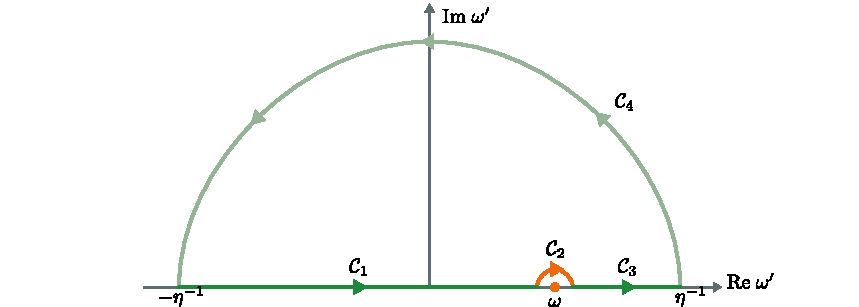
\includegraphics{figs/mt/KK.pdf}
 \caption[Kramers-Kronig contour integral]{ \label{fig:kk}
 \textbf{Kramers-Kronig contour integral.}\small\\
 The contour integral of \eq{kkcontour} can be split into three parts,
 $\mathcal{C}_1 \cup \mathcal{C}_3$ (deep green)
 is the principal value of the integral along the real line;
 $\mathcal{C}_2$ (orange)
 is half the integral around a pole at $\ω$; and
 $\mathcal{C}_4$ (pale green)
 is a contribution that vanishes as the contour limits to infinity.
 }
\end{figure}

A more subtle result that can be derived from the Kramers-Kronig relations is,
that as a function of a complex $\ω$, $\χe(\ω)$ is analytic in the upper
half-plane.
Take the following contour integral,
\begin{equation} \label{eq:kkcontour}
\oint_\mathcal{C}  \d\ω' \:
\frac{\χe(\ω')}{\ω'-\ω}
\;,
\end{equation}
over the closed contour $\mathcal{C}$, where $\mathcal{C}$ is the infinite
semicircle that encloses the upper half-plane, with a infinitesimal semicircular
dent taken out to avoid the pole at $\ω' = \ω$, as shown in \fig{kk},
i.e. $\mathcal{C} = \bigcup_{i=1}^4 \mathcal{C}_i$ with,
\begin{subequations}\subeq
\begin{align}
\mathcal{C}_1 &= [-\η^{-1}, \ω - \η] \\
\mathcal{C}_2 &= \left\{ \ω - \η e^{-i\θ} \middle| \θ \in [0,\π] \right\} \\
\mathcal{C}_3 &= [\ω + \η, \η^{-1}] \\
\mathcal{C}_4 &= \left\{\η^{-1} e^{i\θ} \middle| \θ \in [0,\π] \right\}
\;,
\end{align}
\end{subequations}
in the limit as $\η\→0$.

So long as $\χe(\ω)$ is analytic in the upper half-plane, that is to say there
are no singularities in that region, then \eq{kkcontour} will evaluate to zero.
That is to say,
\begin{equation} \label{eq:kk2}
\int_{\mathcal{C}_1}
+
\int_{\mathcal{C}_2}
+
\int_{\mathcal{C}_3}
+
\int_{\mathcal{C}_4} \d\ω' \:
\frac{\χe(\ω')}{\ω'-\ω}
= 0
\;.
\end{equation}
Contributions from contours 1 and 3 combine to form the principal value of the
integral.
Contour 2 is equal to minus half the residue about the pole
Contour 4 vanishes to zero, which can be understood physically as the
response of a material is unable to match an arbitrarily fast driving term.
This allows the rearrangement of \eq{kk2} as,
\begin{equation}
\PV \int_{-\infty}^{\infty} \d\ω' \:
\frac{\χe(\ω')}{\ω'-\ω}
= \frac{1}{2} 2\π\i \Res\left(\frac{\χe(\ω')}{\ω'-\ω}, \ω\right)
\;.
\end{equation}
which then exactly reproduces \eq{kkComplex}.

This guarantees that the upper half-plane of a causal response function is
analytic, and therefore free of singularities.

\subsection{Drude-Lorentz Model} \label{sec:DrudeLorentz}
One of the most important material models that one can consider is the
Drude-Lorentz model.
It is a causal \cite{Kinsler2011} response that captures the behaviour of most
resonance phenomena.
In its most general terms, it relates the time evolution of $\P$ to a driving
$\E$ field by a second order differential equation:
\begin{equation} \label{eq:tdDL}
\pdd{\P}{t} + \γL\pd{\P}{t} + \ωL^2 \P = \ωp^2 \εf \E
\;,
\end{equation}
where
$\γL$ is a damping term,
$\ωL$ is the restoring force frequency, and
$\ωp$ is the plasma frequency - the coupling strength to the driving $\E$
field.
In frequency domain, one gets,
\begin{equation}
\Ptilde = \εf \frac{\ωp^2}{\ωL^2 - \ω(\ω + i \γL)} \Etilde
\;,
\end{equation}
where the Drude-Lorentz susceptibility can be extracted,
\begin{equation}
\χL(\ω) = \frac{\ωp^2}{\ωL^2 - \ω(\ω + i \γL)}
\;.
\end{equation}
This is analytic in the upper halfplane for $\γL > 0$, and as such obeys the
Kramers-Kronig relations of the previous section.

The origins of a Drude-Lorentz model may vary, and indeed as will be shown
later, a material may host multiple resonances, however, particularly for a
metal, one may explain the origins with a simple model for a free electron gas.
For each electron, let the displacement from its nucleus be given as $\x(\t)$.
A Newtonian force equation can be built from this, using the Lorentz force law,
i.e.,
\begin{equation}
m^* \pdd{\x}{t} = -e \E
\;,
\end{equation}
where $m^*$ is the effective mass of an electron and $e$ is its charge.
Additional forces can be included, such as a collision term proportional to the
velocity and inversely to an average collision time $-\pd{\x}{t}/\τ$.
In this free electron picture, there is no restoring force, though it is
conceivable to add one for electrons bound to a lattice site.
The macroscopic polarisation can be related to these electron displacements, as
each displacement induces an electronic dipole moment, and these can be averaged
to the polarisation by multiplying by the electron number density,
$\P = -e n \x$.
A comparison of terms allows for the mapping,
\begin{equation}
\ωp^2 \→ \frac{n e^2}{m^*} \,,\;
\γ \→ \τ^{-1} \,,\;
\ωL \→ 0
\;.
\end{equation}
This is the Drude model, and with an additional static background permittivity
$\εbg$, it well describes metals.

Real materials typically have multiple resonances, which can be incorporated by
adding multiple Drude-Lorentz resonances,
\begin{equation}
\χ = \sum_i \frac{{\ωp^2}_i}{{\ωL^2}_i - \ω(\ω + i {\γL}_i)}
\;.
\end{equation}
These can have a variety of origins, i.e. in addition to the plasma mode
discussed, rotational modes, electronic transitions, etc.; and indeed the
magnetic response, $\χm$, can also be described as a sum of Drude-Lorentz
resonances.

\section{Transfer Matrix Method} \label{sec:introTMM}
\subsection{Transverse Electric and Transverse Magnetic Solutions}
\label{sec:TETM}
The transverse solutions of \sec{planewaves} can be generalised
to anisotropic media.
Equations~\ref{eq:curlEqs} can be re-written as matrix equations,
\begin{align}
\Etilde = \Z \Zf \Htilde& \\
\Zf \Htilde = \Y \Etilde&
\:,
\end{align}
where $\Z$ and $\Y$ are the impedance and admittance tensors, respectively,
defined as,
\begin{align}
\Z = -\frac{c}{\ω} \εtens^{-1} \crossmat{\Q}& \\
\Y = \frac{c}{\ω} \μtens^{-1} \crossmat{\Q}&
\:,
\end{align}
with $\crossmat{\Q}$ defined as the cross product with $\Q$ expressed as a
matrix.
This allows the electric and magnetic fields to be written as an eigenvalue
equation,
\begin{align}
\Etilde &= \Z\Y \Etilde \\
\Zf \Htilde &= \Y\Z \Zf \Htilde
\:.
\end{align}
The matrix $\Z\Y$ (and $\Y\Z$) has one zero eigenvalue, and by solving for the
other two to be equal to one will give the dispersion relation for two
independent planewave solutions.
The eigenvectors will determine the field polarisation for each solution.

Consider a medium with non-singular permittivity and permeability that are
simultaneously diagonalisable, i.e.,
$\εtens = \diag(\εx, \εy, \εz)$ and $\μtens = \diag(\μx, \μy, \μz)$
in this coordinate system.
Further assume that the wave propagates in a plane normal to the $y$-direction,
i.e. $\Q = (q, 0, \κ)^\TP$.
The resulting two solutions become the basis for
\emph{transverse electric} (\TE) modes,
\begin{subequations}\subeq
\begin{align}\label{eq:TEdisp}
\μx \μz \εy \frac{\ω^2}{\c^2} &- \μx {q}^{2} - \μz {"\κ}^2 = 0 \\
\Etilde &= \EtildeAbs  \left(0, 1, 0\right)^\TP \\
\Zf\Htilde &= \EtildeAbs
\left(-\frac{\c \κ}{\μx \ω}, 0, \frac{\c q}{\μz \ω}\right)^\TP
\;,
\end{align}
\end{subequations}
and \emph{transverse magnetic} (\TM) modes  that will be discussed later in this
section,
\begin{subequations}\subeq
\begin{align}\label{eq:TMdisp}
\εx \εz \μy \frac{\ω^2}{\c^2} &- \εx {q}^{2} - \εz {"\κ}^2 = 0 \\
\Etilde &= \EtildeAbs
\left(1, 0, -\frac{\εx q}{\εz \κ}\right)^\TP \\
\Zf\Htilde &= \EtildeAbs  \left(0, \frac{\εx \ω}{\c \κ}, 0\right)^\TP
\;,
\end{align}
\end{subequations}

\subsection{Planar Boundaries}
Until now we have considered electromagnetic fields in a homogeneous space,
however there is a lot of interesting physics to be found at the boundaries
between different media, and indeed the majority of this thesis considers
surface phenomena.

Consider two infinite half-spaces divided by a planar boundary at $z = 0$.
Let each half-space be filled with a medium, characterised by permittivity and
permeability $\εtens$ and $\μtens$ as described above.
The solutions in each half-space can be assumed to be the same as
those in the homogeneous case for each medium, i.e. planewaves.\footnote{
Strictly, this is only true if the media are local in the direction
normal to the interface.}

It then becomes a question to derive the \emph{boundary equations}
which knit together the solutions at the boundary of the spaces.
To start one takes the Macroscopic Maxwell's Equations, \eq{macME},
and applies Gauss' and Stokes' theorems, to yield their integral form,
\begin{subequations}\subeq
\begin{align}
\oiint_{\partial V} \D \cdot \dS &= \iiint_V \ρext \dV
\\
\oiint_{\partial V} \B \cdot \dS &= 0
\\
\oint_{\partial \σ} \E \cdot \dl &=
 - \pd{}{t} \iint_{\σ} \B \cdot \dσ
\\
\oint_{\partial \σ} \H \cdot \dl &= \iint_{\σ} \Jext \cdot \dσ
 + \pd{}{t} \iint_{\σ} \D \cdot \dσ
\;,
\end{align}
\end{subequations}
Allowing for the possibility of surface charges and currents,
$\ρext = \ρs \δ(z)$ and $\Jext = \Js \δ(z)$,
and taking the volume of integration, $V$, to be a cube of arbitrary $x$,$y$
dimension, but infinitesimally thin in $z$ and straddling the boundary plane,
then,
\begin{subequations}\subeq
\begin{align}
(\Dme_2 - \Dme_1) \cdot \ez &= \ρs \\
(\Bme_2 - \Bme_1) \cdot \ez &= 0
\;.
\end{align}
The surface of integration, $\σ$, is a plane parallel to $z$ and either $x$ or
$y$, again infinitesimal in $z$, this gives the further relations,
\begin{align}
\ez \times (\Eme_2 - \Eme_1) &= 0 \\
\ez \times (\Hme_2 - \Hme_1) &= \Js
\;.
\end{align}
\end{subequations}
Where subscripts 1 and 2 refer to the values of the fields just below and just
above of the interface.

For the planewaves to maintain continuity between each half-space,
they must be of the same frequency, and have the same component of wavevector
parallel to the surface.
Considering the space-time domain solution of a single frequency component,
this restricts the value of the perpendicular component of the wavevector to be
determined by \eqs{TEdisp}{TMdisp}, for which there are two solutions, since
they are equations in $\κ^2$.
The solution in each space is given as,
\begin{equation}\label{eq:EFwBw}
\E =
\begin{cases}
\E_1^+ e^{\i(q x + \κ_1 z - \ω \t)} +
\E_1^- e^{\i(q x - \κ_1 z - \ω \t)} + \cc
& : z < 0
\\
\E_2^+ e^{\i(q x + \κ_2 z - \ω \t)} +
\E_2^- e^{\i(q x - \κ_2 z - \ω \t)} + \cc
& : z > 0
\end{cases}
\;,
\end{equation}
with equivalent solutions for $\H$, $\B$, and $\D$.
The surface charges and currents can be included with the additional
constitutive relation, defining the surface conductivity $\σs$,
\begin{subequations}\subeq
\begin{align}
\Js &= \σs(\q, \ω) \E^\shortparallel (z=0) \\
\ρs &= \σs(\q, \ω) \q \cdot \E^\shortparallel (z=0) / \ω
\;,
\end{align}
\end{subequations}
where the parallel symbol on $\E^\shortparallel$ indicates the $z$ component of
that vector is set to zero, and $\q$ is the $x,y$ plane projection of $\Q$.

To proceed, one needs to consider the \TE and \TM solutions in turn and apply
the boundary value conditions for $z=0$.

For the \TE solution, the non-zero $\E$ and $\H$ field components are $E_y$,
$H_x$, and $H_z$. This though is overdetermined, with
$\Zf H_z = q \c / (\ω \μpar_z)  E_y$.
The boundary value problem can be expressed as a matrix\footnote{
In order to keep $E_y$, $H_x$, and $z$ as a right handed triplet (and for
symmetry with the \TM matrices) the matrix is expressed for (a negative) $-H_x$.
},
\begin{subequations}\subeq
\begin{equation}
\begin{pmatrix}
E_{y2} \\
-\Zf H_{x2}
\end{pmatrix}
=
\underbrace{
\begin{pmatrix}
1 & 0 \\
-\Zf \σs & 1
\end{pmatrix}
}_{\v{S}^\TE}
\begin{pmatrix}
E_{y1} \\
-\Zf H_{x1}
\end{pmatrix}
\;,
\end{equation}
where it can be verified that this also continues the auxiliary fields in the
correct manner.
One may determine the coefficients of the forward and backward propagating waves
in \eq{EFwBw} by expressing it in matrix form for $\x=0$, $t=0$,
\begin{equation}
\begin{pmatrix}
E_{yi} \\
-\Zf H_{xi}
\end{pmatrix}
=
\underbrace{
\begin{pmatrix}
1 & 1 \\
1/\uTE_i & -1/\uTE_i
\end{pmatrix}
}_{\v{U}^\TE}
\begin{pmatrix}
A^+_i \\
A^-_i
\end{pmatrix}
\;,
\end{equation}
with $\uTE_i = \μ_{x i} \ω/(\c \κ_i)$, is the angle dependent\footnote{
For normal incidence, $q=0$, the impedances take the more familiar form,
$\uTE = \sqrt{\μ_x / \ε_y}$ and $\uTM = \sqrt{\μ_y / \ε_x}$.
} impedance,
and $A^\pm_i = \E^\pm_i \cdot \ey$.

The fields can then be calculated at any $z$ coordinate by propagating the
forward and backward components,
\begin{equation}
\left.
\begin{pmatrix}
A^+_{i} \\
A^-_{i}
\end{pmatrix}
\right|_{z}
=
\underbrace{
\begin{pmatrix}
e^{\i \κ_i (z - z')} & 0 \\
0 & e^{-\i \κ_i (z - z')}
\end{pmatrix}
}_{\v{T}}
\left.
\begin{pmatrix}
A^+_{i} \\
A^-_{i}
\end{pmatrix}
\right|_{z'}
\;,
\end{equation}
and of course, at any $x$ and $\t$ by multiplication of $e^{i(q x - \ω \t)}$.
\end{subequations}

The equivalent \TM transfer matrices are given as,
\begin{subequations}\subeq
\begin{align}
\begin{pmatrix}
 E_{x2} \\
 \Zf H_{y2}
\end{pmatrix}
&=
\underbrace{
\begin{pmatrix}
 1 & 0 \\
 -\Zf \σs & 1
\end{pmatrix}
}_{\v{S}^\TM}
\begin{pmatrix}
 E_{x1} \\
 \Zf H_{y1}
\end{pmatrix}
\\
 \begin{pmatrix}
 E_{x i} \\
\Zf H_{y i}
\end{pmatrix}
&=
\underbrace{
\begin{pmatrix}
 1 & 1 \\
 1/\uTM_i & -1/\uTM_i
\end{pmatrix}
}_{\v{U}^\TM}
\begin{pmatrix}
 A^+_i \\
 A^-_i
\end{pmatrix}
\\
\left.
\begin{pmatrix}
 A^+_{i} \\
 A^-_{i}
\end{pmatrix}
\right|_{z}
&=
\underbrace{
\begin{pmatrix}
 e^{\i \κ_i (z - z')} & 0 \\
 0 & e^{-\i \κ_i (z - z')}
\end{pmatrix}
}_{\v{T}}
\left.
\begin{pmatrix}
 A^+_{i} \\
 A^-_{i}
\end{pmatrix}
\right|_{z'}
\;,
\end{align}
\end{subequations}
with $\uTM_i = \c \κ_i / (\εpar_{x i} \ω)$.
These are the matrices of the \emph{transfer matrix method} (\tmm).
The matrices, $\v{S}$, $\v{U}$, and $\v{T}$, in both the \TE and \TM
case, are assigned respectively such that $\v{S}$ continues electric and
magnetic fields from one medium over an interface into another;
$\v{U}$ converts from the basis of forward and backward travelling waves to
electric and magnetic field components;
and $\v{T}$ propagates forward and backward travelling waves from a point $z'$
to a point $z$.

\subsection{Stratified Media} \label{sec:stratmed}

\begin{figure}
 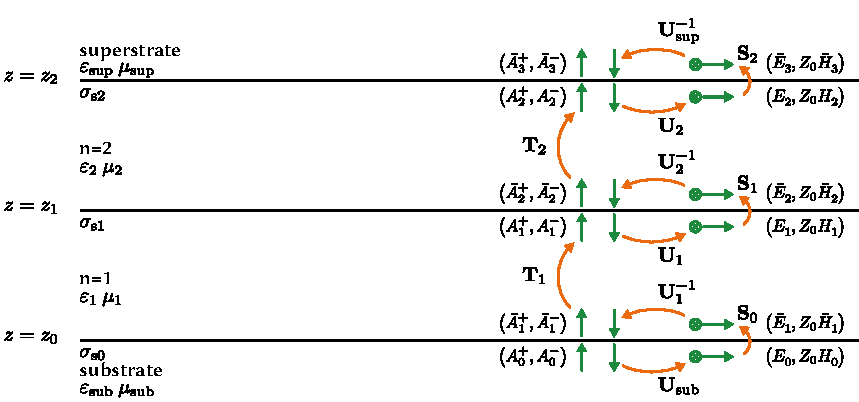
\includegraphics{figs/mt/TMM.pdf}
 \caption[Schematic of the transfer matrix method]{\label{fig:TMM}
 \textbf{Schematic of the transfer matrix method.}\small\\
 Fields (green arrows) are operated on by matrix transformations (orange
 arrows).
 The forward and backward components at the top of substrate layer
 $(A_0^+,A_0^-)$ are transferred through the stack to forward and backward
 components at the bottom of the superstrate layer $(\bar{A}_3^+,\bar{A}_3^-)$.
 Fields move between bases of forward and backward waves (↑ ↓) and
 electric and magnetic components (⊗ →).
 }
\end{figure}

Up until now, this matrix description can be at best described as book-keeping.
Its utility will become clear when generalising to stratified media.
Consider a stack of $N$ planar slabs on a substrate as in \fig{TMM}, each with
its own material properties.
Let the top interface of the $i\th$ slab be at $z_i$, vector
components with that label, e.g. $A^\pm_i$, be measured from there, i.e. just
below the top interface in that layer.
Starting in the forward and backward basis, one may
use the transfer matrices to propagate through the stack from the one layer to
the next.
\begin{equation}
\begin{pmatrix}
A^+_{i+1} \\
A^-_{i+1}
\end{pmatrix}
=
\v{T}_{i+1} \v{U}_{i+1}^{-1} \v{S}_i \v{U}_i
\begin{pmatrix}
A^+_{i} \\
A^-_{i}
\end{pmatrix}
\;.
\end{equation}
The exception to this being the superstrate, the $(N+1)\th$ layer,
which by definition does not have a top interface.
As such $E^\pm_\sup$ is defined specially as the forward and backward
components just above the top interface of the $N\th$ layer, i.e.,
\begin{equation}
\begin{pmatrix}
A^+_\sup \\
A^-_\sup
\end{pmatrix}
=
\v{U}_\sup^{-1} \v{S}_N \v{U}_N
\begin{pmatrix}
A^+_{N} \\
A^-_{N}
\end{pmatrix}
\;.
\end{equation}
The full transfer matrix $\Mtr$ is given as the product of each layer hop,
\begin{equation}
\Mtr = \v{U}_\sup^{-1} \v{S}_N \v{U}_N \dotsm \v{T}_{1} \v{U}_{1}^{-1}
\v{S}_0 \v{U}_\sub
\;.
\end{equation}
Terms with similar indices can be grouped to give a matrix for each layer
\footnote{
Thin film (non-magnetic) layers with thickness $\δ \→ 0$ can be approximated as
$\v{M} \approx \v{S}$, with $\Zf\σs \→ -i\δ(\ω/c) \ε_x$ for \TM and $\Zf\σs \→
-i\δ(\ω/c) \ε_y$ for \TE solutions.
},
\begin{equation}
\v{M}_i = \v{U}_i \v{T}_{i} \v{U}_{i}^{-1}
\;,
\end{equation}
such that the transfer matrix for the whole stack is,
\begin{equation}
\Mtr =
\v{U}_\sup^{-1}
\left( \prod_{i=N}^1 \v{S}_i \v{M}_i \right)
\v{S}_0 \v{U}_\sub
\;,
\end{equation}
noting the reverse order on the product.

The matrix $\Mtr$ maps forward and backward travelling waves in the substrate to
forward and backward waves in the superstrate.
This can be used to calculate reflection and transmission spectra.
Assume a plane wave incident in the superstrate,
this will both reflect at the surface and transmit into the substrate.
This can be codified as a matrix equation, with the assumption that there is no
incoming wave from the substrate,
\begin{equation}
\begin{pmatrix}
r \\ 1
\end{pmatrix}
=
\Mtr
\begin{pmatrix}
0 \\ t
\end{pmatrix}
\;,
\end{equation}
where $1$, $r$, $t$ are the coefficients of the incoming, reflected, and
transmitted components, respectively, of the $E$ field parallel to the stack.
This is solved as,
\begin{subequations}\subeq
\begin{align} \label{eq:reflCoeffs}
t &= (\Mtr_{2 2})^{-1} \\
r &= (\Mtr_{1 2}) / (\Mtr_{2 2})
\;.
\end{align}
\end{subequations}

The coefficients $r$ and $t$ can be used to determine the power flows by the
introduction of the Poynting vector,
\begin{equation}
\S(\x, t) = \E(\x,t) \× \H(\x,t)
\;,
\end{equation}
which is the flux vector of electromagnetic power \cite{Griffiths2013}.
Because it is the product of fields, it is strictly speaking defined only in
space-time domain, however for quasi-monochromatic fields the time-averaged
Poynting vector can be defined as:
\begin{equation}
\left\langle \S \right\rangle = \frac{1}{2} \Re \left(
\E \× \H^*
\right)
\;.
\end{equation}
The component normal to the stacking is of most interest, and in both the \TM
and \TE case, this can be calculated in each layer as,
\begin{equation}
\left\langle \S \right\rangle_z = \Re \frac{1}{2 Z_i \Zf} \left(
|A^+_i|^2 - |A^-_i|^2
\right)
+ \Im \frac{1}{Z_i \Zf} \Im \left( A_i^{+*} A_i^- \right)
\;.
\end{equation}
The first term is power transferred in propagating fields, while the last term
describes power in evanescent fields.

For propagating waves incident in a lossless upper half-plane, the ratio of
reflected and transmitted power flows to the incident power is calculated as,
\begin{subequations}\subeq
\begin{align}
R &= \left.
 \Re \frac{1}{2 Z_\sup \Zf} |A^+_\sup|^2
\middle/
 \Re \frac{1}{2 Z_\sup \Zf} |A^-_\sup|^2
\right.
\\ 
T &= \left.
 \Re \frac{1}{2 Z_\sub \Zf} |A^-_\sub|^2
\middle/
 \Re \frac{1}{2 Z_\sup \Zf} |A^-_\sup|^2
\right.
\;.
\end{align}
\end{subequations}
In in terms of the coefficients of \eq{reflCoeffs}, this reads,
\begin{subequations}\subeq
\begin{align}
R &= |r|^2
\\ 
T &= \frac{\Re Z_\sub^{-1}}{\Re Z_\sup^{-1}}|t|^2
\;.
\end{align}
\end{subequations}

One point has been so far glossed over: the branch of the square
root of $\κ^2$.
Both positive and negative solutions are included, but to identify one or the
other as forward or backward travelling waves, one must chose $\κ$ such that
$\Re \κ > 0$ in the superstrate.
In the substrate the situation is more complicated, since the waves may be
either propagating or evanescent here.
If $\κ$ is real, pick the positive root,
but if it is complex or imaginary, it must be picked such that $\Im \κ > 0$,
This will guarantee that fields exponentially decay from the surface rather
than diverging.

\subsection{Surface Plasmon Polariton}

With the transfer matrix, one is also able to calculate the bound modes of a
system.
These are the eigenmodes of the system which have non-zero fields for a zero
driving field, i.e.,
\begin{equation}
\begin{pmatrix}
A^+_\sup \\ 0
\end{pmatrix}
=
\Mtr
\begin{pmatrix}
0 \\ A^-_\sub
\end{pmatrix}
\;,
\end{equation}
with the prescription that $\Im \κ > 0$ in both the super- and substrate, such
that fields on both sides decay away to infinity.
This yields the condition that $\Mtr_{2 2} = 0$ for bound modes.
In general this is satisfied for either one of the frequency $\ω$ or wavevector
$q$ being a complex number, with the other remaining real.

Here the example of the surface plasmon polariton (\spp) is considered, a mode
that exists on the interface between a metal and an insulator, where charge
carriers on the metal's surface couples to the electric field.
\textsc{Spp}s are of interest because, as will be shown, they permit field
solutions which extend beyond the diffraction limit, allowing for high
confinement of electromagnetic energy and large field enhancement at the
interface.

Consider a metal substrate and dielectric superstrate, the metal
characterised by a dispersive permittivity $\εpar(\ω)$ and the dielectric by a
static constant $\εD$.
Both layers are non-magnetic, $\μpar = 1$, and there is no external surface
conductivity $\σs = 0$.
S\textsc{pp} modes are \TM in nature, so we shall only seek these solutions.
It can be shown that \TE \spp solutions do not exist \cite{book:Maier}.

In this case the transfer matrix is given as,
\begin{subequations}\subeq
\begin{align}
\Mtr &= \v{U}_\sup^{-1} \v{U}_\sub
\\
 &=
\frac{1}{2}
\begin{pmatrix}
 1 & \frac{\c \κ_\sup}{\εD \ω} \\
 1 & -\frac{\c \κ_\sup}{\εD \ω}
\end{pmatrix}
\begin{pmatrix}
 1 & 1 \\
 \frac{\εpar(\ω) \ω}{\c \κ_\sub} & -\frac{\εpar(\ω)  \ω}{\c \κ_\sub}
\end{pmatrix}
\;,
\end{align}
\end{subequations} 
which gives the \spp condition,
\begin{equation}
\Mtr_{2 2} = \frac{1}{2}
\left( \frac{\c \κ_\sup}{\εD \ω} \frac{\εpar(\ω) \ω}{\c \κ_\sub} + 1 \right)
 = 0
\end{equation}
\begin{equation}
\frac{\εpar(\ω)}{\εD} + \frac{\κ_\sub}{\κ_\sup} = 0
\;.
\end{equation}
One can see that for this equation to have solutions, given $\εD > 0$ and $\Im\κ
> 0$, then it must hold that $\Re \εpar(\ω) < 0$, which is characteristic of
metals for frequencies below their plasma frequency.

For a lossless Drude metal, i.e. $\εpar(\ω) = \εinf- (\ωp/\ω)^2$, an analytical
solution exists,
\begin{equation}
q^{2} = \εD \left(\frac{\ω}{\c}\right)^2
\frac{
 \εinf \ω^2 - (\εD + \εinf) \ωsp^2
}{
 (\εD + \εinf)(\ω^2 - \ωsp^2)
}
\;,
\end{equation}
where $\ωsp = \ωp / \sqrt{\εD + \εinf}$, is the \emph{surface plasmon
frequency}.

For small wavevectors, the dispersion relation becomes
$\ω \→ q c / \sqrt{\εD}$, where it follows the dielectric medium
lightline.
As the wavevector increases, the curve shall become shallower than the light
line and as $q\→\infty$, the dispersion relation tends to the limiting value
$\ω \→ \ωsp$.
Here the \spp transitions between being photonic in character to becoming like a
\emph{surface plasmon}, where the field limits to being entirely confined to
the surface.
The diffraction limit is surpassed here as an arbitrarily large wavevector range
is supported at a small frequency range, in the limit of no loss.

In this thesis, multi-layer structures will be considered that support hybrid
\spp modes about one or multiple material interfaces.
In general, analytical dispersion relation solutions do not exist, but rather
solutions for $\Mtr_{2 2}(\q, \ω) = 0$ are found implicitly, using a
root-finding algorithm.

\section{Finite Difference Time Domain} \label{sec:fdtd}
\begin{figure}
 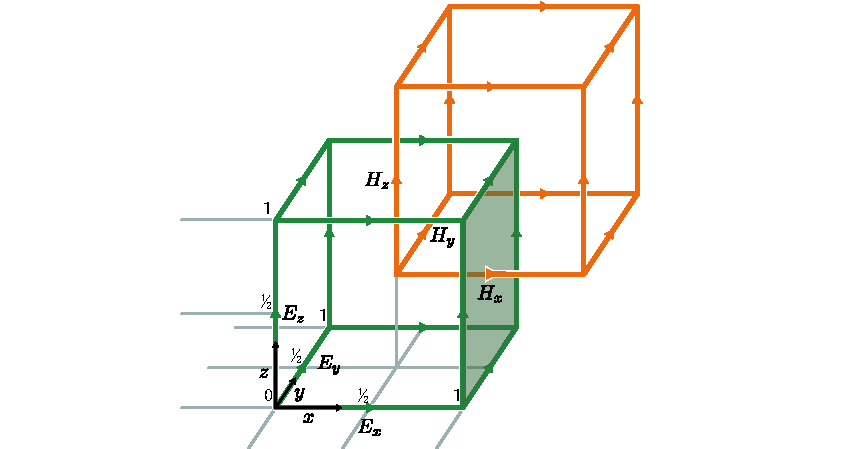
\includegraphics{figs/mt/FDTD.pdf}
 \caption[Schematic of \fdtd Yee cell]{ \label{fig:FDTD}
 \textbf{Schematic of \fdtd Yee cell.}
 Electric (green) and magnetic (orange) field grids.
 They are shifted half a step from each other, forming an interlocking link.
 Each field line passes through the centre of a square formed from lines of the
 other field, e.g. $H_x$ here passes through the centre of the highlighted
 $E$-field face, where the finite difference $\curl \E$ is defined.
 }
\end{figure}

The real world exists in time domain; whereas the frequency domain is
mathematically complementary, the purpose of calculations done in it must
ultimately be to get a handle on the time evolution of a system.
As the complexity of a system increases, analytic methods begin to get less and
less tractable.
In order to complement such techniques, numerical simulations may be employed.
In this thesis, the \emph{finite difference time domain}
(\fdtd) method \cite{Yee1966,Taflove1995} will be used.

In \fdtd, the goal is to solve Maxwell's equations for successive instants in
time over a discretised lattice.
This is approached by taking the curl equations, and making the time derivatives
of the fields the subject.
Making the assumption that there are no external sources,
\begin{subequations}\subeq
\begin{align}
\pd{\E}{\t}  &= \frac{1}{\εf} \left( \curl \H - \pd{\P}{\t} \right) 
\\
\pd{\H}{\t}  &= -\frac{1}{\μf} \left( \curl \E -\pd{\M}{\t} \right) 
\;.
\end{align}
\end{subequations}
Now, space and time are discretised as
$(t, x, y, z) \→ ( n\Δt, i\Δx, j\Δx, k\Δx )$ and
derivatives are turned into finite differences, i.e.,
\begin{equation}
\pd{\E}{t}(\x, t) \→ \frac{\E^{n+1}_{i, j, k} - \E^n_{i, j, k}}{\Δt}
\;.
\end{equation}
Strictly, the above is a central difference and approximates the time derivative
at a time $(n+1/2)\Δt$.
Therefore the corresponding right-hand-side terms must be evaluated at
this time.
The curl operator is handled similarly,
\begin{equation}
\curl \E(\x, t)|_x \→ \frac{E_z|^n_{i, j+1, k} - E_z|^n_{i, j, k}}{\Δx} -
\frac{E_y|^n_{i, j, k+1} - E_y|^n_{i, j, k}}{\Δx} \;.
\end{equation}
In order to make best of this central difference, the lattice is arranged as
a Yee grid \cite{Yee1966}, where fields are stored separately by component and
$\E$ and $\P$ fields are specified on integer time coordinates, whereas $\H$ and
$\M$ are specified on half integer time coordinates.
The lattice coordinates are more complicated, for $\E$, components are stored
at half-integer coordinates in their own direction and at integer coordinates
otherwise.
This is the opposite for the $\H$ field, as illustrated in
\fig{FDTD}.
From here, one can write the \emph{update equations},
\begin{subequations}\subeq
\begin{align}
E_x|^{n+1}_{i+\½, j, k} &= E_x|^n_{i+\½, j, k}
- \εf^{-1} P_x|^{n+1}_{i+\½, j, k} + \εf^{-1} P_x|^n_{i+\½, j, k}
\\ \nonumber
&+ \frac{c\Δt}{\Δx}
\left(
  \Zf H_z|^{n+\½}_{i+\½, j+\½, k} - \Zf H_z|^{n+\½}_{i+\½, j-\½, k}
\right)
\\ \nonumber
&- \frac{c\Δt}{\Δx}
\left(
  \Zf H_y|^{n+\½}_{i+\½, j, k+\½} - \Zf H_y|^{n+\½}_{i+\½, j, k-\½}
\right)
\\
\Zf H_x|^{n+\½}_{i, j+\½, k+\½} &= \Zf H_x|^{n-\½}_{i, j+\½, k+\½}
+
c M_x|^{n+\½}_{i, j+\½, k+\½} - c M_x|^{n-\½}_{i, j+\½, k+\½}
\\ \nonumber
&+ \frac{c\Δt}{\Δx}
\left(
  E_z|^{n}_{i, j+1, k+\½} - E_z|^{n}_{i, j, k+\½}
\right)
\\ \nonumber
&- \frac{c\Δt}{\Δx}
\left(
  E_y|^{n}_{i, j+\½, k+1} - E_y|^{n}_{i, j+\½, k}
\right)
\;,
\end{align}
\end{subequations}
with corresponding equations for the omitted components.

With the update equations of the primary fields determined, it remains to
describe how the auxiliary fields update.
In general, the constitutive equations are functionals of all past values of all
fields, as described in \sec{constitutive} and \sec{KKrels}, though this would
prove tricky to directly implement.
In practice, material responses can be cast in terms of a finite difference if
they can be expressed in terms of a temporal differential equation.
This lends the Drude-Lorentz model of \sec{DrudeLorentz} well to inclusion
within \fdtd, though it's update equations and how to incorporate them are
beyond the scope of this thesis.

The \fdtd algorithm therefore proceeds by iterating over updating in order the
$\E$ field, $\M$ field, $\H$ field, and $\P$ field over all space for each
timestep.

There are limitations to \fdtd.
Its staggered grid structure means that material interfaces are not sharply
defined, and any curvature on an interface will also experience a staircasing
effect that can lead to spurious hot-spots especially in plasmonic structures
where geometric effects play a key role.
The grid is also regular, which is to say it can not be adaptively refined in
areas of interest, rather all points must be simulated to the same resolution.
This adds to the numerical load, as the smallest wavelength component of the
fields, as well as the smallest geometrical features must be provided with
sufficient resolution.
This is again especially relevant in plasmonics, where field confinement is a
feature.

Because of its nature as a full wave time domain solver, \fdtd can often be the
final say on a theoretical investigation.
Short of doing a real-world experiment, \fdtd numerical simulations find their
utility as a heavy-duty tool.
That is, the Maxwell's equations are solved at every discretised point in space,
so it is often slower and more cumbersome, but can as a result of the inherent
thoroughness produce results for questions that other techniques are unable to.

\section{Evolutionary Algorithm} \label{sec:EA}

\begin{figure}
 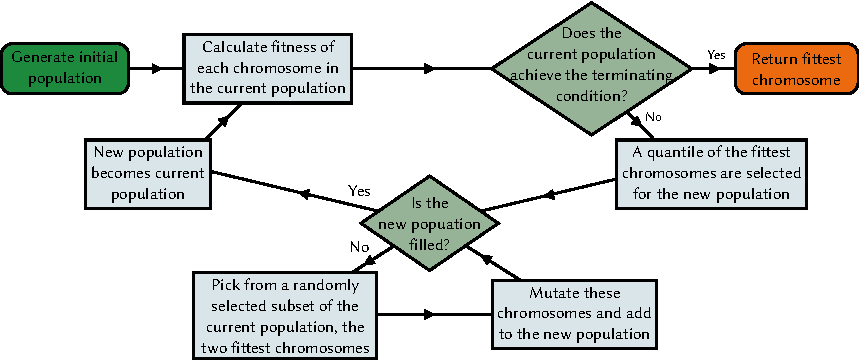
\includegraphics{figs/mt/Flow.pdf}
 \caption[Evolutionary algorithm flowchart]{\small \label{fig:flow}
 \textbf{Evolutionary algorithm flowchart.}
 }
\end{figure}

For a planar stratified structure whose properties can be determined by a
transfer matrix method, one may wish to optimise some aspect of its response to
electromagnetic radiation.
This may be in the dispersion relation of bound modes or in the transmission and
reflection spectra.
For example, to prescribe the frequency of a bound mode, or a
reflection peak; or set whether there is only a single mode or
many modes within a frequency range; or control the amplitude and phase response
to an incoming wavepacket.
These properties are entirely determined by the composition of the structure,
however it often not obvious how changes in the structure lead to changes in the
response.

The structures to be considered can be described by a finite number of numeric
or discrete parameters, i.e. for each layer: the thickness of the layer, the
material model to use, and the parameters of that model.
This is well suited to optimisation using an \emph{evolutionary algorithm}
(\ea) \cite{Spears2000}.

In brief, an \ea operates by storing multiple copies of these parameter sets,
perturbing the values of the parameters randomly, ordering the sets by how the
system they describe performs against a fitness metric, and keeping only the
best variants to the next round.

More fully, in the language of an \ea, this would be to say that a
\emph{population} of \emph{chromosomes} is kept, and on each iteration of the
algorithm, new chromosomes are generated from \emph{mutations} of the current
ones, the next generation population is filled by \emph{selection} of these
chromosomes by a \emph{fitness function}.
The goal of the \ea is to find a chromosome which extremises the fitness
function globally, and as such an \ea is most suitable when the evaluation of
the fitness function can be performed relatively quickly as a large number of
members of the state space must be evaluated and compared.

A chromosome is simply the set of parameters which describes a system, i.e.
a list of numbers or discrete option values.
They are atomic entities, independent of other chromosomes.
Each chromosome may have its fitness function evaluated to determine how
suitable its corresponding physical system is to a problem.

Each iteration of the \ea holds a set of chromosomes, ordered by their fitness
function, known as a \emph{population}.
The first generation is seeded population either
with randomly generated structures, or structures that have been tuned by hand,
perhaps by approximative theoretical methods.
Populations of subsequent generations are constructed by firstly taking a small
quantile of the fittest chromosomes from the previous iteration, with the
remaining places filled with \emph{mutations} of chromosomes selected from the
previous set.
The progress of the algorithm can be tracked by examining the fittest chromosome
at the end of each iteration.
At the end of each iteration, a \emph{terminating condition} is evaluated, which
determines if the algorithm should stop, returning the fittest chromosome, e.g.
if the best structure in the population is within a defined tolerance of the
target output, or if a set number of iterations have elapsed.
If the terminating condition is not met, then the algorithm continues for
another iteration.
The operation of the \ea is described as a flowchart in \fig{flow}.

The mutation process generates a new chromosome by randomly perturbing the
values of parameters of a parent chromosome.
It is by mutation that the state space of chromosomes is mapped.

For the layered structures considered here, the mutation process will perturb
both the properties of the layers themselves, and the relationship between
layers.
Numeric parameters, such as layer thicknesses and those used in material
models are perturbed by a Gaussian random variable, and the discrete
parameters, such as the layer model, can be randomly selected from a list.
Typically only one or few parameters will be changed in each mutation.
The parameters of the layers themselves don't sit in isolation.
The number of layers in these structures is variable and mutation
allows for adding or removing of layers or indeed swapping the order of layers
and shifting the boundary between adjacent layers.

Whereas the \ea is widely applicable to problems in nano-optics,
the fitness function is not general and has to be constructed for each problem
based on what characteristics are to be selected for.
In \sec{SLOptimisation} a fitness function will be defined for structures that
hold light in a bound mode at zero group velocity, seeking to reduce the
dispersion of a wavepacket propagating in the structure.
 % Chapter 2 - Methods
\clearpage~\clearpage
\chapter{Plasmonic Stopped Light Lasing}

\section{Introduction} \label{sec:sllIntro}
The speed at which light travels in vacuum is a fundamental property of the
universe and is the upper limit on the speed at which energy can be
transferred.
This speed is outside the scale of normal human experience, and in the context
of nano-optics is considerable at 299.792458 μm/ps.
This high speed does present a problem when storing light-energy, however;
light does not readily slow down.
In the presence of polarising or magnetising media, light will be slowed by a
factor defined as the \emph{refractive index}, which typically is no larger than
about 5, with the largest bulk refractive index known being that of a
metamaterial with an index of 33 \cite{Choi2011}.

The reduction in speed can be improved on by considering the wave nature of
light, and in a chosen frequency interval, modifying the
\emph{dispersion relation} of a wavepacket through resonant phenomena.
This is the field of inquiry of \emph{slow} or \emph{stopped light} (\sl), and
is studied within a broad range of research areas from where the resonant
phenomena can be derived \cite{Khurgin2005}.
These range from
\emph{electromagnetically induced transparency} in cold atom gases
\cite{Hau1999,Liu2001,Lukin2001,Boyd2009}
and in solid state devices
\cite{Ibanescu2004,Yanik2004,Ibanescu2005,Zhang2008,Papasimakis2008},
to \emph{periodic backreflectance} in photonic crystal structures
\cite{Vlasov2005,Krauss2007,Baba2008}
semiconductor quantum wells \cite{Ku2004},
and \emph{Goos-Hänchen shift} \cite{Berman2002} in negative refractive index
metamaterial structures \cite{Tsakmakidis2007,Kirby2011}.
These approaches are not without issues to overcome.
Applications in optical information processing would require integrated
structures operating under ambient conditions, which limits the utility of cold
atom gases in this context.
Photonic crystals rely on periodic structuring, where stopped light resonances
are vulnerable to imperfections and disorder, reducing the speeds to
hundredths of the vacuum velocity but falling short of complete stopping
\cite{Mookherjea2007,Engelen2008}.
Metamaterials, on the other hand, require operation to be on lengthscales where
the meta-atoms are effectively homogenised \cite{Smith2004}, and require
intricate patterning within these scales \cite{Zhang2005,Valentine2008}, though
the chief problem with metal based metamaterials is Drude loss
\cite{Stockman2007,Kinsler2008}.

In this thesis, stopped light is considered in the context of planar
nanoplasmonic structures \cite{Karalis2005}.
Plasmonic stopped light is also robust against disorder, as shown in
Ref.~\cite{Tsakmakidis2014}, but will not be discussed in detail here.
Whereas plasmonic structures are still susceptible to Drude loss faced in the
metamaterial case, this can be compensated for by the inclusion of a gain
material.
Finally, the composition of such plasmonic structures is simple and lends
itself well to experimental realisation.

Stopped light brings about an enhanced density of states \cite{Yao2009} and
allows for the localisation of light coherently over long timescales, which can
enhance nonlinear effects \cite{Franken1961} and interaction with active
components \cite{Lakowicz2004,Fu2011}, making stopped light relevant for
applications in the light harvesting of solar cells
\cite{Aubry2010,Jang2011,Callahan2012}, quantum
information processing \cite{Liu2001}, and optical memories \cite{Zhang2009} as
well as applications in optical communications \cite{Mok2005}.

One of the implications of stopped light, that is perhaps its most interesting,
is \emph{stopped light lasing}.
When designing a laser there are, broadly, two components that must be
considered - gain and feedback.
Gain is the mechanism by which photons (or indeed plasmons) are generated by
stimulated emission.
Here a photon will induce the relaxation of an electron from one state to
another of lower energy, and crucially, emit a second photon that is coherent
with the first.
This process can be repeated, and while the electron population is inverted
(that is there are more electrons in the upper rather state, rather than the
lower), will grow the number of photons in a
coherent state exponentially.
The gain media that are available include semiconductors in bulk
\cite{Kenyon2002}, quantum dots \cite{Plum2009} and wells \cite{Carrere2006},
as well as organic laser dye molecules \cite{Sperber1988}.

Feedback, on the other hand, is the means by which the photons emitted are
coupled back to interact with the same gain medium, such that they may stimulate
further emission.
Most lasers will use a resonant cavity for this purpose, where the cavity modes 
localise electromagnetic energy over a gain medium.
In the field of nanolasing there have been many such examples including
photonic crystal defect modes \cite{Painter1999,Altug2006}, microcavity
resonators
\cite{Iga1988,McCall1992,Vahala2003},
and even the multiple scattering of a “random laser”
\cite{Cao2003,Wiersma2008}.

Stopped light offers an alternative mechanism for feedback than with a cavity.
\sl modes are only confined in one spatial dimension, and not in the other two.
This permits a continuum of planewave solutions, i.e. \sl modes are
propagating waves, rather than standing waves, albeit at zero group velocity.
The lasing mode of a stopped light laser forms dynamically, based on the gain
support for the continuum of modes instead of being predetermined by the
geometry of a cavity.
Here the feedback is provided by a balance of adjacent forward and backward
power flows that form a closed-loop optical vortex which gives rise to the zero
group velocity.

In this chapter, we seek \emph{stopped light structures}, these are
heterogeneous media, whose dispersion relations have at least one zero group
velocity point, i.e. $\Re \dd{\ω}{q} = 0$ for some finite values of the
wavevector $q$.
In such structures, wavepackets of light are pinned and do not drift away
albeit still propagating with a finite phase velocity.
Though to spatially confine light over long timescales, it is not enough
just to have a zero group velocity, one needs to also minimise the dispersion
and material losses.

The energy confinement of stopped light provides the basis for the feedback
mechanism required for lasing to occur.
Nanoplasmonic stopped light lasing is shown to provide a robust mechanism for
the ultrafast excitation of coherent surface plasmon polaritons from simple,
experimentally realisable, subwavelength structures.

\subsection{Organisation of chapter}
This chapter is structured as follows:
In \sec{pvgvd} the dispersion relation of light is explained, introducing
phase, group, and dispersion velocities.
This is followed by a discussion of the differences between a complex frequency
and complex wavevector picture of dispersion in \sec{cwcf}.

The features that make a good stopped light structure, how to find and optimise
structures that possess these, and finally how to excite stopped light modes are
presented in \sec{plasSLS}.
An optimised structure is then analysed in frequency domain, including how
plasmon modes can become undamped with the inclusion of a gain medium in
\sec{fdGain}.

Time domain simulations are performed in \sec{tdSims}.
These are based on a four level system model for the gain (\sec{4lvl}).
\Sec{lasingDynamics} investigates how the lasing mode is onset as gain density
is increased, for a stopped light structure and a non-stopped control
structure.
Then in \sec{lasingMode} the spatial and temporal characteristics of the lasing
mode is examined as the width of the gain medium is reduced, exploring the
confinement and output of the lasing mode.

The results are summarised and the chapter is concluded in \sec{slConc}.

\section{Phase Velocity, Group Velocity, and Dispersion} \label{sec:pvgvd}

\begin{figure}
 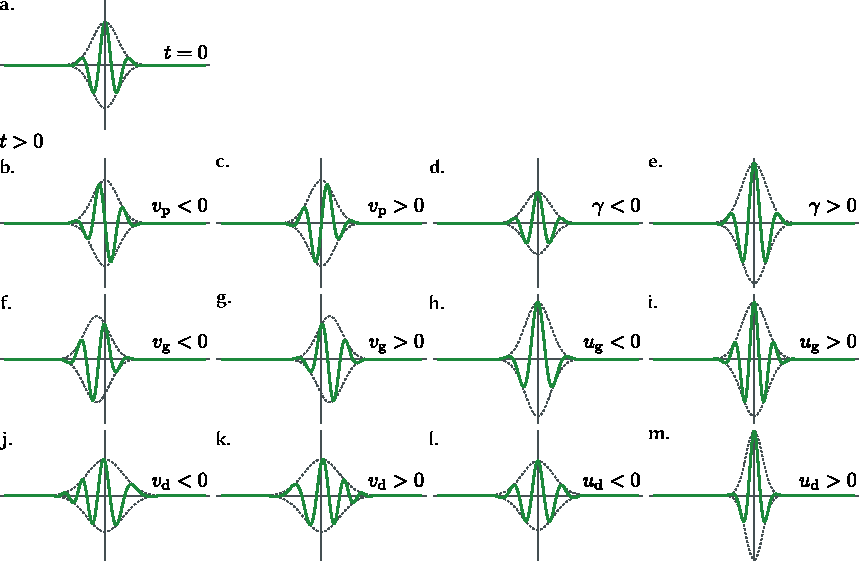
\includegraphics{figs/sl/Disprel.pdf}
 \caption[Effect of moments of the dispersion relation]{\label{fig:Disprel}
\textbf{Effect of moments of the dispersion relation.}\small\\
A Gaussian enveloped planewave at $t=0$, \subA, is shown individually under the
effects of the moments of the dispersion relation for $t>0$.
Subfigures are paired to have a negative then positive value of an individual
moment, with all others set to zero.\\
\subB, \subC. phase velocity $\vp$ -
envelope remains constant as phase advances.\\
\subD, \subE. loss $\γ$ -
amplitude of the envelope decreases/increases.\\
\subF, \subG. group velocity $\vg$ -
envelope shifts as phase remains constant.\\
\subH, \subI. group loss $\ug$ -
amplitude of envelope increases as phase wavelength increases/de\-creases.\\
\subJ, \subK. dispersion velocity $\vd$ -
envelope widens and a negative/positive chirp is induced.\\
\subL, \subM. dispersion loss $\ud$ -
envelope widens/narrows with no chirp.
}
\end{figure}

Before entering into a study of particular plasmonic stopped light structures,
we first explore how a wavepacket propagates under a
dispersion relation $\ω(q)$, and how its shape evolves as it does.
This will have implications, as will be shown, for the lateral confinement of
such a wavepacket within a finite area.

Consider a wave propagating in one dimension $x$,
with a well defined wavevector, $q_0$, and a narrow spatial bandwidth,
$\σ_0^{-1}$, which gives it a slowly varying spatial envelope with a width
$\sim\σ_0$,
Then the dispersion relation is well described by its Taylor expansion to second
order about $q=q0$,
\begin{equation}
\ω(q) = \vp q_0 + \vg (q - q_0) + \vd\frac{\σ_0}{2} (q - q_0)^2 + \ldots
\;,
\end{equation}
where the following velocities are introduced\footnote{
If three separate velocities seems a lot, in 1977, S.~C.~Bloch reviews seven
previously identified velocities of light in dispersive media and introduces his
own eighth
\cite{Bloch1977}.
} in place of the usual derivative Taylor coefficients:
\emph{phase velocity}, $\vp = \ω(q_0)/q_0$,
\emph{group velocity}, $\vg = \ω'(q_0)$, and
\emph{dispersion velocity} $\vd = \ω''(q_0)/\σ_0$.

A Gaussian wavepacket following this prescription has the functional form,
\begin{equation} \label{eq:tZeroGauss}
\φ(x) = \exp \left(
-\frac{x^2}{2\σ_0^2} + i q_0 x
\right) + \cc
\end{equation}
at a single instant in time, $t=0$.
In order to calculate the time evolution of the wave packet, the function needs
to be expressed in the Fourier domain, where the dispersion relation applies,
\begin{align}
\tilde{\φ}(q) &= \frac{1}{2\π}\int_{-\infty}^{\infty} \d x \: \φ(x) e^{-i q x}
\\
&= \frac{\σ_0}{\sqrt{2\π}} \exp \left(
-\frac{\σ_0^2(q-q_0)^2}{2}
\right)
\;.
\end{align}
In this basis, the time evolution is simply given by multiplication by the
propagator $e^{-i \ω(q) t}$,
\begin{equation}
\tilde{\φ}(q,t) = \tilde{\φ}(q) e^{-i \ω(q) t}
\;.
\end{equation}
The wavepacket then becomes,
\begin{align}
\tilde{\φ}(q,t)
&= \frac{\σ_0}{\sqrt{2\π}} \exp \left(
-\frac{(\σ_0^2 + i \vd\σ_0 t)(q-q_0)^2}{2}
- i \vg (q - q_0) t
- i \vp q_0 t
\right)
\;,
\end{align}
which when transformed back, yields the form,
\begin{equation}
\φ(x,t) = \sqrt{\frac{1}{1+i \vd t / \σ_0}} \exp \left(
-\frac{(x-\vg t)^2}{2(\σ_0^2 + i \vd\σ_0 t)} + i q_0 x - i \ω_0 t
\right) + \cc
\end{equation}
or,
\begin{align} \label{eq:tdGaussian}
\nonumber
\φ(x,t) &=
\φ_0(t) \exp \left(
-\frac{(x-\vg t)^2}{2\σ(t)^2}
\right)
\exp \left(
i q_0 (x - \vp t )
\right)
\\
&\× \exp \left(
i\frac{(x-\vg t)^2}{2\σ(t)^2}
\frac{\vd t}{\σ_0}
\right)
\\ \nonumber
&+ \cc
\end{align}
with the following definitions made:
$\σ(t)^2 = \σ_0^2 + (\vd t)^2 $, and
$\φ_0(t) = \sqrt\frac{\σ_0^2 - i \σ_0 \vd t}{\σ(t)^2}$.

Examining \eq{tdGaussian} term by term;
the first two exponential terms determine that this is a Gaussian function that
is modulated with a planewave of wavevector $q_0$, as in \eq{tZeroGauss}.
The modulation now has a \emph{phase velocity} $\vp$, and the envelope is
centred on $\vg t$, a point that moves in time with the \emph{group velocity}
$\vg$.
The width of the Gaussian increases over time, as determined by $\σ(t)$, which
increases over time proportionally to the \emph{dispersion velocity} $\vd$
and decreases the peak amplitude of the pulse as it spreads, as determined by
$\φ_0(t)$.
The final term is a complex phase factor that determines the \emph{chirp} of the
wave, which at any instant in time, gives a spatial factor
$\exp(i q_\mathrm{c}^2 x'^2)$ (for $x' = x - \vg t$, and $q_\mathrm{c}$ is a
time-dependant constant), which is a complex phasor with a wavelength that
decreases away from a central point.
Another way to envisage this is, when the dispersion relation has a positive
curvature, the local group velocity $\dd{\ω}{q}(q)$ is higher for larger
wavevectors than for small ones, as such higher wavevector components make
their way to the front of the wavepacket, leaving the low wavevector components
at the back.

The previous analysis has presented the time evolution as though the dispersion
relation were real valued, whereas in general, each of the moments has an
imaginary part, which will be denoted as,
\begin{equation}
\ω(q) = \Re \ω(q)+ i\γ + i\ug (q - q_0) + i\ud\frac{\σ_0}{2} (q - q_0)^2
+ \ldots
\;.
\end{equation}
For even order moments $\γ$ and $\ud$, the loss and dispersion loss, positive
values represent gain whilst negative represent loss. The odd moment $\ug$, the
group loss, is alternatingly gainy or lossy either side of the central
wavevector, with the effect of shifting the central wavevector over time .
The effect of all the moments of the dispersion relation is plotted in
\fig{Disprel}.
%need a better name for group loss.

The resulting expansion of a Gaussian pulse evolution is lengthy, therefore its
explicit expression will be omitted here.
The group loss and dispersion loss terms each contribute to the complex phase of
the wavepacket, though this will not be explored further.
The effect on the amplitude however is to multiply by an exponential factor
and to apply a spatial convolution by an additional broadening term\footnote{
For this second order Taylor expansion model to remain valid, the loss
dispersion, $\ud$ should satisfy, $\ud \le 0$ and $|\ud| \gtrsim |\ug|$.
},
\begin{equation}
\φ(x,t) \→ \exp\left(\γ t - \frac{\ug^2}{2\ud\σ_0} t \right) \times 
\frac{\exp\left( \frac{x^2}{2 \σ_0 \ud t} \right)}{|\σ_0 \ud t|}
\otimes_x
\φ(x,t)
\;.
\end{equation}
These additional terms are present because the imaginary part of the dispersion
relation will change the profile of the wavevector spectral density over time,
\begin{equation}
|\φ(q, t)|^2 \propto e^{2[\Im \ω(q)] t}
\;.
\end{equation}
This is in contrast to the real moments of the dispersion relation, which do not
alter the spectral density.

This section has explained how the dispersion relation affects the
space-time propagation of band-limited electromagnetic radiation.
By engineering the dispersion relation, via choice of materials and structuring,
one may seek to control the pulse propagation itself.
This is to include control over the shape of a pulse, and how it drifts
and disperses, but also the phase relations and chirping.

\section{Complex Wavevector and Complex Frequency} \label{sec:cwcf}
The dispersion relation of the modes of a planar heterostructure, as discussed
in \sec{stratmed}, is determined as the condition required to maintain a
nonzero electromagnetic field within a structure in the absence of an external
driving field.
The solutions are planewaves in a direction of propagation perpendicular to the
stacking of the heterostructure, i.e. $\exp(i q x - i \ω t)$, and the
dispersion relation is the range of allowed $q$ and $\ω$ value pairs.
The dispersion can, of course, be expressed in functional form as either
$q_i(\ω)$ or $\ω_i(q)$, where $i$ is the mode index.
The functions are called the \emph{complex wavevector} (\cwv) and
\emph{complex frequency} (\cfr) representations, respectively.
In general both quantities are complex, but expressing them in functional
form allows for the function argument to be given as a real eigenvalue
parameter.
Both descriptions are equivalent, and describe the same space time dynamics.

Consider a structure with a single mode, with a monotonic dispersion relation.
Its spacetime profile can be expressed in the complex wavevector picture as,
\begin{equation}
  \φ(x,t) = \int_{-\infty}^{\infty} \d\ω \:
  \tilde{\φ}(\ω) e^{i q(\ω) x - i \ω t}
\;,
\end{equation}
which could be interpreted at face value as in integral along the real axis, or
alternatively as a complex contour integral along the path $\ω(s)$,
\begin{equation}
  \φ(x,t) = \int_{-\infty}^{\infty} \d s \:\dd{\ω}{s}
  \tilde{\φ}(\ω(s)) e^{i q(\ω(s)) x - i\ω(s) t}
\;.
\end{equation}
If the path is chosen such that $q(\ω(s)) = s$ for all $s \in \reals$,
then the integral becomes,
\begin{equation}
  \φ(x,t) = \int_{-\infty}^{\infty} \d s \:
  \tilde{\φ}(s) e^{i s x - i\ω(s) t}
\;,
\end{equation}
with $\tilde{\φ}(s) = \tilde{\φ}(\ω(s)) \dd{\ω}{s}$,
and this is exactly the complex frequency representation, as parameterised by a
real wavevector $s$.
The mode's spectral content $\tilde{\φ}(\ω)$ is analytically continued from
the real axis to the curve $\ω(s)$.

Given the equivalence of the two pictures, the utility of each must be
discussed.
The complex frequency picture is parameterised with a real wavevector
eigenvalue;
this means that it is a description suited to having a wavepacket with a known
spatial distribution at one instant in time, and calculating the time evolution,
i.e. having energy stored in a structure and calculating how it dissipates.

The complex wavevector picture on the other hand, is suited to knowing the time
evolution of a wavepacket at a single point in space, and then calculating the
propagation of the wave through space. e.g. calculating propagation in a
fibre-optic cable with a known signal input at one end.

For stopped light, it is the complex frequency representation that is the most
useful.
This can be justified both intuitively and mathematically.
Intuitively, we will want to determine the propagation of a wavepacket
with losses at the zero group velocity point.
It makes little sense to consider the complex wavevector (losses in space)
picture as, by construction, we are considering wavepackets that do not
propagate in space.
Conversely losses in time are indeed a meaningful quantity for a stationary
wavepacket.

Mathematically speaking, for a structure with at least one stopped light point,
i.e. where $\Re \dd{\ω}{q} = 0$ for a finite $q$,
this is just a turning point in an $\ω(q)$ description, whereas in a $q(\ω)$
picture, this is a singular point, and multiple branches of the function must be
considered to capture the behaviour about the point.

In practice, stopped light points don't even manifest themselves in the complex
wavevector solutions \cite{Reza2008,Yao2009}, therefore from here on, the
complex-frequency picture is used to analyse the \sl modes of structures
under consideration.

Though the complex-wavevector picture can not describe stopped light itself, it
will be shown that it is well suited to describing the plasmons that are
emitted as an output channel from stopped light lasing.

\section{Plasmonic Stopped Light Structures} \label{sec:plasSLS}
%Figure showing zgv point and flatness

In order to confine light longitudinally in a waveguide, a wide range of
wavevectors must be supported within a narrow frequency range.
A way of achieving this would be to use a structure that supports two
\emph{zero group velocity} (\zgv) points on the same mode.
A \zgv point defines a turning point in the real part of the
dispersion relation, i.e. $\Re \dd{\ω}{q}(q_0) = 0$.
By definition, having two adjacent \zgv points implies that the
dispersion relation in-between is necessarily monotonic, since no further
turning points can exist within the interval.
It is also guaranteed that a point of zero dispersion, $\Re \ddd{\ω}{q} = 0$,
(see \sec{pvgvd}) exists in the range.

The range of wavevectors between the two \zgv points is referred to as a
\emph{stopped light band}.
The quality of such a band will be determined by two factors,
how narrow the frequency bandwidth is, and how broad the wavevector bandwidth
is.
For a pair of stopped light points \zgv1 and \zgv2, the frequency and wavevector
bandwidths are given as $\Δω = \ω_2 - \ω_1$ and $\Δq = q_2 - q_1$ respectively.
This allows for the definition of the \emph{band velocity} $\vb$,
which is the average group velocity between the \zgv endpoints,
\begin{equation}
\vb = \frac{\ω_2 - \ω_1}{q_2 - q_1} = \frac{\Δω}{\Δq}
\;.
\end{equation}
The wavevector bandwidth determines the minimum width that a light
pulse can be confined to, i.e. $\sim 2\π / \Δq$, whereas the frequency
bandwidth will set the overall flatness of the band, and additionally ensures
the operation of the stopped light device to remain quasi-monochromatic, which
becomes important as the stopped light mode is coupled to inverted emitters in a
narrow frequency band (see \sec{fdGain}).

For this study, we consider structures with materials characteristic of a
\threefive semiconductor, i.e. InGaAsP for dielectric layers, and a
transparent conducting oxide \cite{Naik2013}, such as Indium Tin Oxide (\ito)
for metallic layers.
The dielectric is modelled with a constant permittivity
$\ε = 11.68$.
\textsc{Ito}, which has a plasma resonance in the visible which can be
tuned by doping, allowing for operation in the near infrared (i.e. at
telecoms wavelength [$\λ\approx1550\nm$]). It is modelled by a Drude model with
parameters as given in \tab{4lvlParams} provided by experimental data
\cite{Noginov2011}, with the loss reduced by a factor of 10,
which can be achieved through high fabrication quality and at low
temperatures \cite{Khajavikhan2012}.

\subsection{Mode Hybridisation} \label{sec:hybrid}

\begin{figure}
 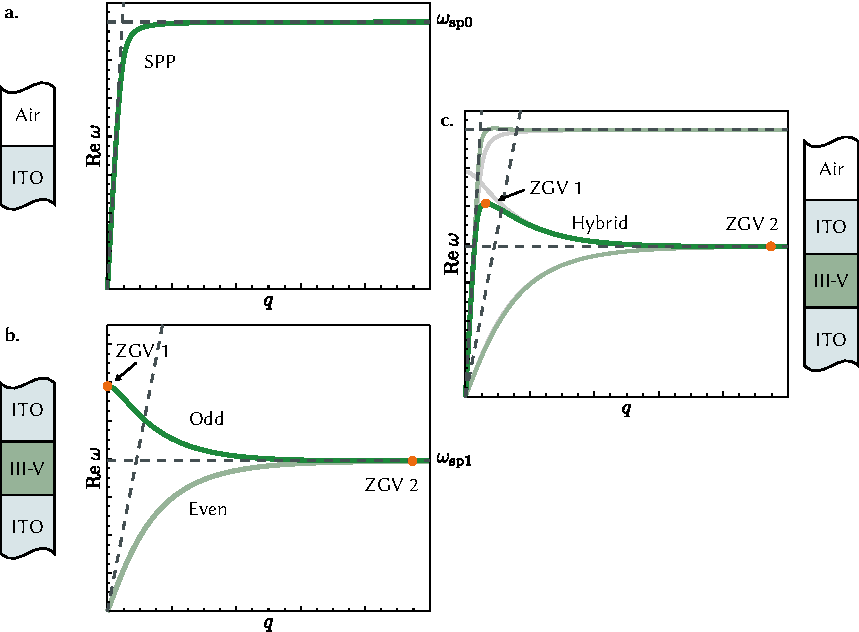
\includegraphics{figs/sl/HybridMode.pdf}
 \caption[Hybridisation of modes]{\label{fig:HybridMode}
\textbf{Hybridisation of modes.}\small\\
Dispersion relations, $\Re \ω(q)$, are plotted, with the asymptotic light lines
in vacuum $\ω = c q$, and in dielectric $\ω = c q / \εbg^2$, and
surface plasmon frequencies, ${\ωsp}_0 = \ωp/\sqrt{\εinf+1}$ and ${\ωsp}_1 =
\ωp/\sqrt{\εinf+\εbg}$.
Modes of interest are highlighted in deep green, and \zgv points marked in
orange.
\subA. The \spp mode of a metal-air interface, is hybridised with \subB. the odd
mode of a metal-insulator-metal structure, \subC. forming a
metal-insulator-metal-air structure in order to produce a mode with two zero
group velocity points at finite wavevector.
The modes of the “base structures” are included in the background of \subC.
to show the hybridisation.
}
\end{figure}

The dispersion of plasmonic structures is ultimately determined by how its
layers are composed, i.e. their thickness, material, and relative
ordering.
It is possible to predict, and even control, how the dispersion relation will
look before explicitly calculating it.
Having such a model becomes useful in reducing the search space of optimisation
methods discussed in the next section, since calculating the
dispersion relation consists of solving a transcendental equation, which requires
numerical methods.

The predictive power stems from the spatial profile of the plasmonic
mode having peaks on metal/dielectric interfaces with exponential tails,
\begin{equation}
\φ(z) \propto
\begin{cases}
\exp\left( -\Im\κ_+(q) (z-z_0) \right) & z > z_0 \\
\exp\left( \Im\κ_-(q) (z-z_0) \right) & z < z_0
\end{cases}
\;,
\end{equation}
where $\Im\κ(q) > 0$, and broadly increases with $q$.
For small values of $q$, the tails are broad and the mode overlaps with the rest
of the structure, whereas for large $q$ the mode only sees the interface which
it sits at.
Each metal/dielectric interface hosts a surface plasmon, and at low
wavevectors they will overlap and hybridise, while for high $q$ they will
decouple.

This was shown in Ref.~\cite{Karalis2005} with a metal substrate underneath two
dielectric layers, a high index beneath a low index dielectric.
The dispersion relation initially followed the steeper plasmon dispersion of the
metal/low-index overshooting the lower frequency of the asymptotic
metal/high-index surface plasmon frequency which it would tend to for high
wavevectors.
This produced a \zgv point between the two regimes, that was somewhat tunable
by the thickness of the middle layer.

A similar approach can be used for introducing \emph{two} stopped light points.
The two modes to hybridise are that of a \emph{metal-insulator-metal}
(\mim) system \cite{Economou1969}, and a \emph{metal-air} (\ma) plasmon.
The structures and dispersion relations are plotted in \fig{HybridMode}.
The \mim system has two modes, even and odd;
the odd mode (in the $z$ component of the $\E$-field) contains two \zgv points
itself, the first one is at zero wavevector and is not useful being inside the
light cone, the second one is at a high wavevector near where the even and odd
modes become degenerate, and is preserved.

In the combination structure, that is a \emph{metal-insulator-metal-air} (\mima)
system, the odd mode of the \mim system hybridises with the \ma plasmon,
removing the zero-wavevector \zgv point but introducing a new point in the
overlap.
The second \zgv point can also be perturbed and gets pulled in to a lower
wavevector value, depending of the precise structural configuration.

The positions of the \zgv points can be tuned by adjusting the thicknesses of
each layer, while further fine control can be attained by introducing additional
dielectric layers \cite{Karalis2009a}.

\subsection{Evolutionary Optimisation} \label{sec:SLOptimisation}

\begin{figure}
 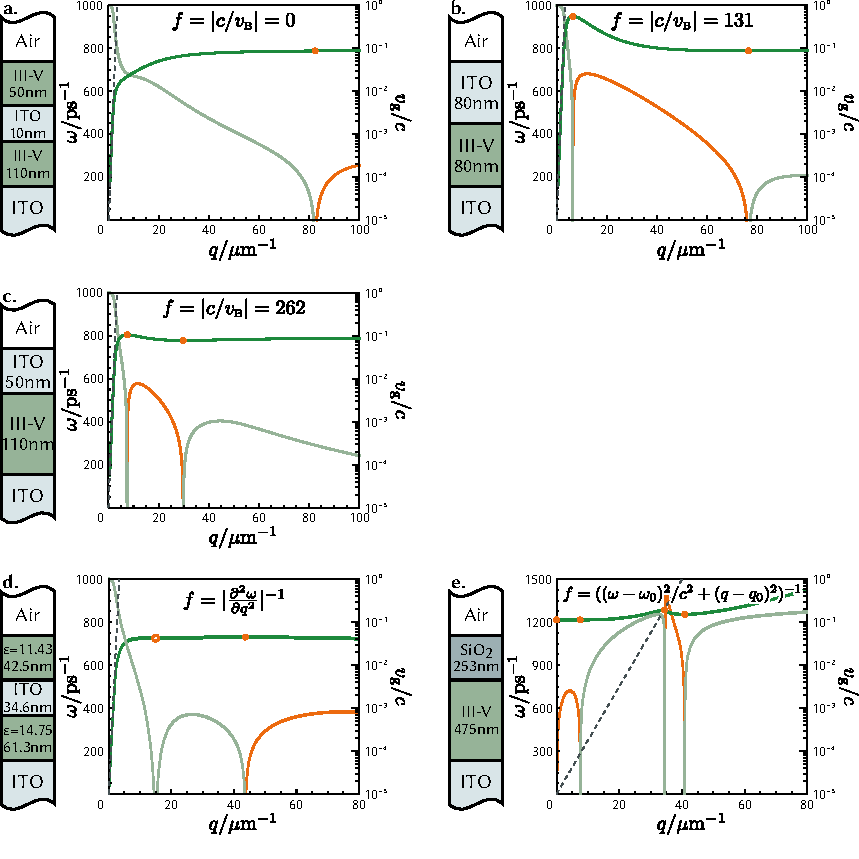
\includegraphics{figs/sl/GA.pdf}
 \caption[Evolutionary optimisation of stopped light structures]{
 \label{fig:GA}
\textbf{Evolutionary optimisation of stopped light structures.}\small\\
The dispersion relation, group velocity, and fitness metric of a number of \sl
structures. \subA, \subB, and \subC. are tested against the band velocity
metric.
\subD. and \subE. are examples of structures tested under alternate metrics and
with relaxed conditions on materials and layer thicknesses, i.e. (d) Minimising the
second derivative (dispersion) at a \zgv point, (e) Placing the \zgv point at
$q=1\nm^{-1}$, $\ω = 2\π\c/1550\nm$ for a \emph{leaky mode}.
}
\end{figure}

Any given stopped light structure can be optimised using an evolutionary
algorithm, as detailed in \sec{EA}.
The algorithm is seeded with a structure that already has two stopped light
points in one band, as prescribed in the previous section.
The algorithm then generates a number of similar structures, and for each, the
dispersion relation of the corresponding band is calculated.
The structures are assigned and ordered by a fitness metric, where
structures without two \zgv points are flauchinauchinihilipilificated and
immediately discarded. The remaining structures are then passed through the \ea
routine for mutation, recombination and selection.
For the purpose of identifying \zgv points, only the real part of the group
velocity is required to be zero, this is despite the dispersion relation itself
being complex (see \sec{pvgvd}) as it is the real part that determines the shift
of the mode over time.

In order to quantify the quality of a stopped light structure, a fitness metric
must be defined and calculated.
In general this is a functional of the dispersion relation, $f[\ω(q)]$,
(either over the whole curve, or just between the \zgv points).
In practice though, this can be reduced in complexity, and it suffices to just
consider a function of the bandwidths $f(\Δq, \Δω)$.
The landscape of their possible values needs to be considered and how changes in
both variables makes a more or less desirable structure.

The band velocity on face value would seem to be a suitable parameter, as,
\begin{equation} \label{eq:fitnessfn}
f(\Δq,\Δω) = 1 / |\vb|
\;.
\end{equation}
A subtlety does however arise, in that the second \zgv point can tend towards
an infinite value of $q_2$ for finite $\ω_2$, This will send the band velocity
to zero, but allows for an arbitrarily large frequency bandwidth.
To counteract this, a high wavevector cutoff is introduced at around
$\qc\approx 2\π/10\nm$, which modifies the wavevector bandwidth to
$\Δq' = \max(q_2,\qc) - q_1$ which then enters the metric.

Three candidate \sl structures are contrasted in \fig{GA}.
Each of them representing a \threefive{} / \ito heterostructure, but with
varying layer configurations, each layer optimised to the nearest $10\nm$.
The first is an example of a structure with a single stopped light point, which
would be rejected by this particular configuration of the \ea as it fails to
possess two \zgv points, and hence cannot be assigned a fitness metric.
The second structure possesses two \zgv points and covers a wide range of
wavevectors, hence represents a good candidate with a fitness metric of
$f = 131 / c$.
The third structure is an optimised version of the previous one with a lower
band velocity, giving a fitness of $f = 262 / c$.
Albeit its \zgv points are closer together in $q$, there is a smaller frequency
gap, which results in a band velocity around half of its predecessor.
The gradient of the bands can be seen from the dispersion diagram, the
dispersion in \figSub{GA}{.c} exhibits a much flatter band than in \subB.

Two further structures are presented, these have been optimised by the \ea but
with less strict constraints and with different fitness metrics.
The first seeks to minimise the dispersion, $\pdd{\ω}{q}$ at a \zgv
point, rather than the band velocity.
This effectively brings two \zgv points to coalescence rather than spreading
them out, which doesn't guarantee a wide band.
Here a third \zgv point appears in the vicinity of the first
two, this does not contribute directly to the metric, but does make an overall
stronger \sl structure.
The disadvantage to this approach, is that a \emph{second order} \zgv point is
fragile;
Akin to the repeated root of a quadratic equation, a perturbation of parameters
could lead to either two separate \zgv points, or indeed none at all.
Structures can only be tuned to a degree before fabrication tolerances and
disorder will smear their properties.

The second additional structure is one which considers \emph{leaky modes}, where
the fields in the air layer are exponentially growing, rather than decaying,
and the bound modes appear within the light cone.
Leaky modes optimised by this method were analysed for the \emph{photonic}
structure presented in Ref.~\cite{Pickering2014}.
For the structure in \FigSub{GA}{.e}, the target was to place a \zgv point at
telecoms frequency $\ω = 2 \π \c / 1550\nm$ at a wavevector of $q = 1\μm^{-1}$.
i.e. $f = ((\ω-\ω_0)^2/c^2 + (q-q_0)^2)^{-1}$.
This structure used the material properties of Silicon and Silicon Dioxide in
two dielectric layers, with arbitrarily precise thicknesses.
Whereas this structure will not be considered here, as its modes are photonic
in character, a case which has been treated separately \cite{Pickering2014}, it
serves to illustrate the versatility of the \ea for designing structures.

\begin{figure}
 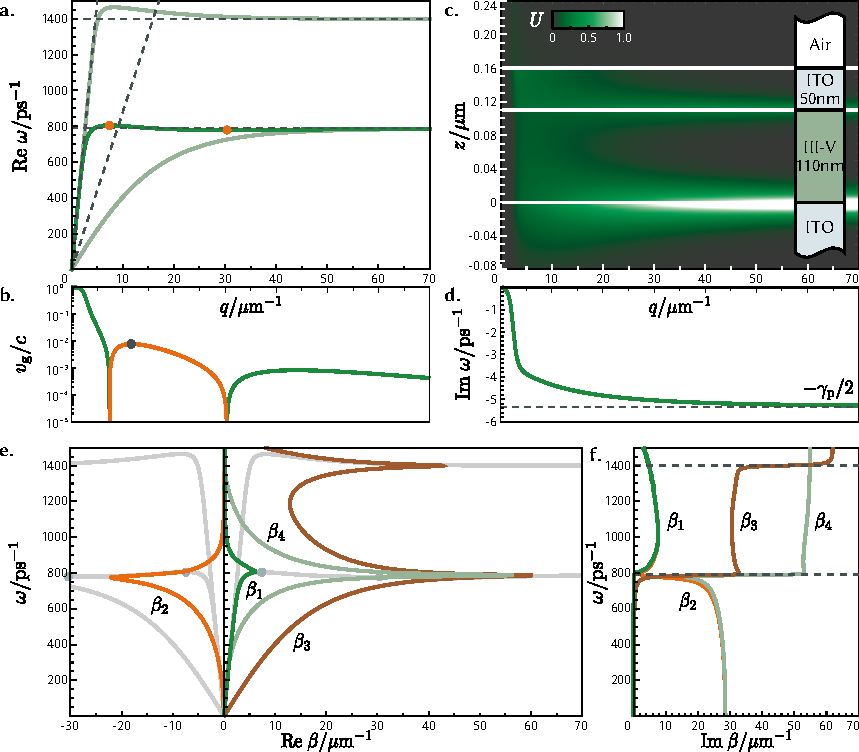
\includegraphics{figs/sl/Dispersion.pdf}
 \caption[Dispersion relation of a stopped light structure]{
 \label{fig:Dispersion}
\textbf{Dispersion relation of a stopped light structure.}\small\\
\subA. Complex frequency mode dispersion relations - The mode of interest is
highlighted in deep green and its \zgv points marked as orange dots.
Also marked are the light line and surface plasmon frequency, both for the
vacuum and dielectric.
\\
\subB. Group velocity log plot of the mode of interest - Positive group
velocities in green, negative in orange. The point of zero dispersion is marked
in grey.
\\
\subC. Description of the structure and energy density throughout the structure
of a planewave of wavevector $q$ in the bound mode.
\\
\subD. Modal loss, $\Im \ω(q)$, up-to the limiting value of $-\γp/2$.
\\
\subE. Complex wavevector modes $\Re \β(\ω)$ - The first four modes are plotted,
the second mode (orange) is of negative phase velocity.
The complex frequency modes are plotted in the background to show the
correspondence.
\\
\subF. Modal loss, $\Im \β(\ω)$, of corresponding complex wavevector modes.
}
\end{figure}

The optimised \sl structure that is used within the rest of the chapter is
presented in more detail in \fig{Dispersion} with properties in \tab{slprops}.
It is composed of an \ito substrate on the bottom, and a
semiconductor layer sandwiched between an \ito strip on top with layers
optimised to the nearest $10\nm$ The modes of this structure are shown alongside
in \figSub{Dispersion}{.b}, and indeed the bound \TM1 mode hosts two \zgv
points.
As a result it exhibits a very flat band with a band velocity of $\vb =
-c/262$.
The mode profile of the energy density of a planewave in the mode is
also shown in dependence of the wavevector $q$.
Being plasmonic in nature, the field is peaked on the interface between the
metallic and dielectric layers, and for low $q$ values, where the
dispersion follows the light cone, it is primarily located in the air layer,
entering the structure for higher $q$ values.
The field has significant value throughout the profile of the dielectric layer
for wavevectors between around $q \in [0.002,0.025] \nm^{-1}$, i.e. while the
plasmons that sit on either side of the dielectric are coupled.
This enhancement of fields is important for stopped light lasing, as it provides
a large overlap between the field profile and an embedded gain medium.

For completeness, the \cwv modes are also presented in \fig{Dispersion}.
To avoid confusion with the \zgv points of the \cfr modes, the complex
wavevector is labelled $\β$ rather than $q$ as previously.
There are an infinite range of \cwv modes, each with increasing imaginary
component; the first four are listed here.
The modes map to the \cfr set in particular places on the dispersion curve, but
pick up large loss where they diverge.

Having, to a large degree, removed the effects of drift and dispersion from our
system, by choosing one with a wide flat band, we are left with loss as the
mechanism that will hinder energy confinement.
For all wavevectors where the dispersion relation departs from the light line,
the system experiences a loss of around $-2 \Im \ω \approx \γp \approx
11\ps^{-1}$.
This will dissipate any energy within the system on such a timescale.
Naturally, the question arises, whether the loss be compensated for, such as by
replacing the dielectric layer with a semiconductor medium, or by explicitly
adding emitters such as quantum dots or gain molecules.

\subsection{Excitation of Stopped Light Modes}
Once a suitable stopped light structure has been selected, the next step is to
excite the stopped light mode.
The usual methods for coupling to a plasmonic waveguide become unsuitable in the
stopped light case.
Bound modes by definition are not coupled to external radiation modes, which is
to say that light energy cannot be transferred to a bound mode by a beam
of light incident on the surface.
This is also linked to the secondary reason, that there is a mismatch
between the wavevector of incident light and the bound modes of a plasmonic
structure, along the direction of propagation\footnote{
The wavevector component normal to the stack is not conserved, so it suffices to
consider the projection in the propagation direction
}.
Incident light is located exactly on the light cone in
energy-momentum space and has a projection in the propagation direction within
it, whereas plasmonic modes are on a line that sits outside the light cone, and
indeed need not be bounded at all in momentum.

In plasmonic structures, one method of coupling is achieved by adding a
local spatial inhomogeneity, such as a prism, or a grating.
In the case of the prism, light is sent down the prism, within the prism's
shallower light cone ($q \le n\ω/c$), this allows for points where the energy
and momentum of both the incoming beam, and the plasmon mode match
\cite{Otto1968}.
In addition to this condition, the prism must be finite in extent, as the
incoming light is part of the radiation spectrum of the “waveguide with prism”
system that will ultimately by transmitted, reflected, or absorbed.
This mode will mix with both the radiation modes and bound modes of the
“waveguide without prism” system, and will decouple from the prism further down
the waveguide.

A grating, which is a periodic patterning of the waveguide along the propagation
direction, acts in a similar way \cite{Ritchie1968}.
The regular patterning allows for scattering between wavevector modes
that are integer multiples of the grating wavevector, $2π/d$, where $d$ is the
period.
This gives a \emph{momentum kick} to the incident light field, allowing it to
match with the dispersion relation of the bound mode.
Again, the radiation mode of the “waveguide with grating” system then mixes with
the bound and radiation modes of the “waveguide without grating”.

These methods are ineffective with stopped light structures because the bound
mode has a low group velocity such that the incident light is unable to get
sufficiently far away from the grating or prism and instead is outcoupled back
through the radiation modes of the combined structures, instead of travelling
far enough for the system to be described by modes without a grating or prism.

Another scheme for incoupling light to a waveguide is end-fire coupling
\cite{Stegeman1983}.
Here the waveguide is assumed to terminate in a plane perpendicular to the
direction of propagation.
If a light pulse is incident on this terminal plane, its profile can be
decomposed into a mixture of bound modes and radiation modes of the waveguide;
the radiation modes propagate away, leaving the bound modes in the system.
This too is unsuitable for exciting stopped light modes, as zero group velocity
modes will not propagate down the structure, they will not enter and instead be
reflected back.
This method of excitation is equivalent to using the complex wavevector
picture, where the temporal profile of excitation at one point along the axis
(the terminal) is known, but as explained in \sec{cwcf}, \zgv points
are not well described in the complex wavevector picture.

A final way to excite the bound modes of a plasmonic waveguide, that is
compatible with stopped light,
is to have them emitted directly from within the structure.
Here, an emitter would be placed within the \sl structure and these would be
pumped to an excited state, such that when they relax, by spontaneous or
stimulated emission, they are able to emit directly into the bound stopped
light mode.

\section{Frequency Domain Gain in the Small Signal Gain Regime}
\label{sec:fdGain} Adding gain to a structure will alter the bound modes that
are supported.
A material that can spontaneously emit photons will also be available to emit
via stimulated processes, thereby adding gain to the system.
This gain will be dispersive in two senses, firstly different frequencies
experience different amounts of gain, and secondly any change to the imaginary
part of the refractive index (i.e. the material gain) will in turn induce a
change in the real part of the refractive index due to causality and the
Kramers-Kronig relations (\sec{KKrels}).
Designing an active \sl structure requires particular care that the introduction
of a gain medium does not damage the stopped light character of the waveguide.

The induced change in mode structure can be analysed using the same transfer
matrix methods of the previous section with the inclusion of a Lorentz
resonance (\sec{DrudeLorentz}) at a defined emission frequency, $\ωe$, to one of
the dielectric layers.
The Lorentz resonance represents the transitions between the levels of a
two-level system with an energy difference $\ħ\ωe$.
In this picture, there is an occupation density of upper and lower levels,
averaged over space, of single two level emitters.
The strength of the resonance is proportional to the \emph{inversion
density} of the two levels, i.e. how much more the higher level is occupied
than the lower one, $\ΔN = N_2 - N_1$, such that a layer with emitters embedded
may be represented by :
\begin{subequations}\subeq
\begin{align}
\ε &= \εbg + \frac{\ωpe^2}{\ωe^2 - \ω(\ω + i \γe)} \\
\ωpe^2 &= -\ΔN \sqrt{\εbg} \γe \σe c
\;,
\end{align}
\end{subequations}
where
$\εbg$ is the permittivity of the layer hosting the resonance, 
$\σe$ is the emission cross-section,
and $\γe$ is the width of the resonance \cite{Wuestner2010}.
Note that for negative inversion, the emitter becomes an absorber as there is a
higher density of emitters in the lower state.

\begin{figure}
 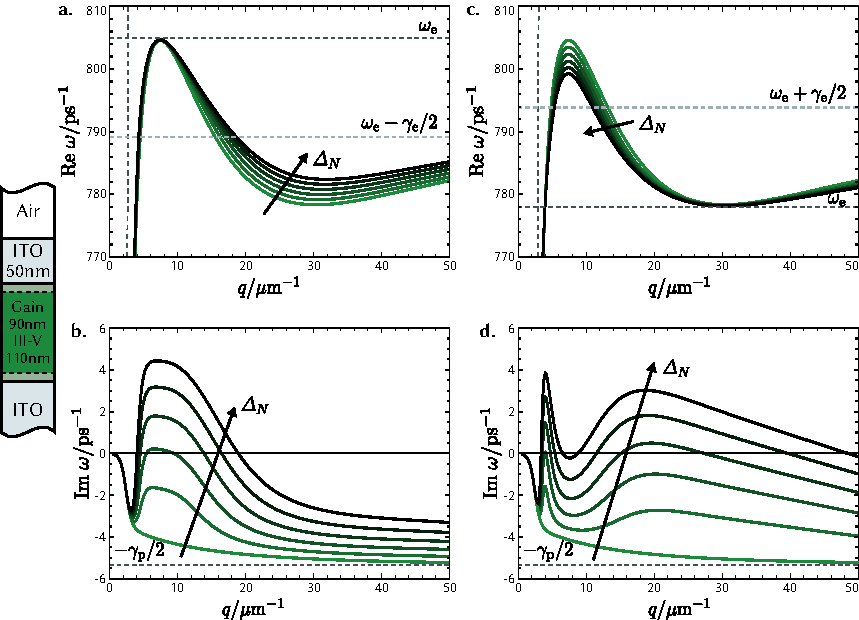
\includegraphics{figs/sl/FdGain.pdf}
 \caption[Perturbation of dispersion relation and loss with Lorentzian
 gain]{
 \label{fig:FdGain}
 \textbf{Perturbation of dispersion relation and loss with Lorentzian
 gain.}\small\\
 The change of mode shape is plotted as Lorentzian gain is introduced to the
 system. For subfigures on the left, emission is about \zgv1, and on the right
 about \zgv2.
 \subA. and \subB. shows a zoom in of how the dispersion relation changes with
 increasing inversion density, while \subC. and \subD. show the corresponding
 loss/gain of the mode.
}
\end{figure}

The \sl structure as presented in the previous section is modified by replacing
the dielectric layer with a Drude-Lorentz emitter (with a $10\nm$ buffer on
both ends of zero inversion density to simulate quenching by the metal layer).
The emission frequency is set to match either one of the \zgv points, and the
other parameters are set as in \tab{4lvlParams} representing the inclusion of
realistic laser dye molecules \cite{Sperber1988}.
The resulting dispersion and loss relations are shown in \fig{FdGain} for
inversion densities $\ΔN$ varying between $0$ and $N$, with a fixed
emitter density, and excitation about \zgv1 and \zgv2.
The first point of note is that, even on full inversion, the addition of gain
does not significantly change the dispersion, with the maximum shift in
frequency being around $0.6\%$.
The presence of \zgv points is preserved, though they may drift slightly, i.e.
\zgv2 moves slightly right with emission about \zgv1.
There is no change at the frequency that is being excited, this
is because the permittivity change of a Lorentzian is zero at the resonant
frequency.
Adding gain has the side effect of making the structure a slightly better
\sl structure as the band velocity is marginally reduced.

The key change though is in the loss.
As the inversion density increases, the loss decreases for wavevectors where the
dispersion is within the gain width.
Initially the plasmons loss is reduced as the inversion increases, then for
an inversion of around $\ΔN/N \approx 0.4$ some wavevectors become undamped, and
even eventually experience gain, Plasmons sitting in these modes will grow
exponentially in amplitude whilst small enough to remain in the
small signal gain regime.
As \zgv2 is flatter than \zgv1, when the emission is about this point, a wider
range of frequencies fall within the gain width, leading to a larger range of
$q$ values that can become undamped.

\section{Time Domain Simulations} \label{sec:tdSims}
A frequency domain analysis can only bring insight so far when describing
processes such as gain, as it is unable to describe nonlinearities.
When plasmons are emitted, electrons are demoted
from higher energetic states to lower ones.
This depletes the population inversion,
reducing the available gain over time, leading to nonlinear dependence in the
field strength.
In addition there are spatial effects to consider, such as spatial hole
burning; the \tmm has assumed uniformity in the direction of propagation,
whereas the level of inversion can vary both in this direction and
perpendicular to the stacking.
Depending on the mode formed, some regions may host higher field densities which
can deplete the local gain.
Thus a dynamic, spatially resolved, time domain simulation is required to
capture all the aspects of emission into a stopped light mode, and as such, in
this section results from \fdtd simulations are presented.

\subsection{Four-Level System} \label{sec:4lvl}

\begin{figure}
 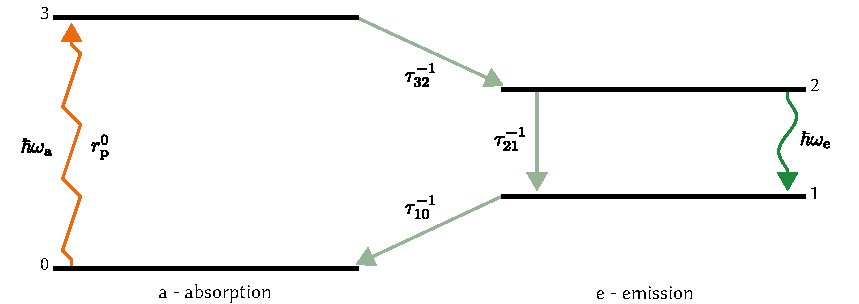
\includegraphics{figs/sl/4lvl.pdf}
 \caption[Schematic of the four-level system]{\label{fig:4lvl}
\textbf{Schematic of the four-level system.}\small\\
 A four-level system is composed of two two-level systems, $\mathrm{a}$ and
 $\mathrm{e}$, with active transitions (0 ↔ 3) and (1 ↔ 2) respectively,
 which are coupled by nonradiative transition rates
 $\τ_{32}^{-1}$ and $\τ_{10}^{-1}$.
 In this scheme, the emission subsystem permits radiative transitions at an
 energy of $\ħ\ω$ and has a slow nonradiative recombination rate
 $\τ_{21}^{-1}$, while the absorption subsystem is electrically pumped at a
 constant rate $\rp$.
}
\end{figure}

The two level system, presented in the previous section, is good for modelling a
single electronic transition, however its inversion density had been set “by
hand”.
There is no way in which a two level system can reach a state of inversion
by relying solely on the processes of spontaneous emission and absorption (the
best that can be achieved is equal occupation of the levels).
A \emph{four-level system} on the other hand can be constructed such that there
can be a dynamically maintained population inversion between two of its levels,
from where stimulated emission can occur.
The construction contains two two-level systems, labelled $\mathrm{e}$ and
$\mathrm{a}$ for emission and absorption; $\mathrm{e}$ is a system with
energy levels 1 and 2 and energy gap $\ħ\ωe$, in-between $\mathrm{a}$, a
system with energy levels 0 and 3 and greater energy gap $\ħ\ωa$, as depicted
in \fig{4lvl}.
The two upper levels, 2 and 3 are coupled by a fast nonradiative
relaxation channel, with rate $\τ_{32}^{-1}$, as are the two lower levels, 0 and
1 ($\τ_{10}^{-1}$).
This has the effect of rapidly depleting the 1\st and 3\rd level shortly after
they become occupied.
Between the levels of the emission two-level subsystem, there is
additionally a slow nonradiative channel ($\τ_{21}^{-1}$).

The key point of a four-level system is that electrons that are pumped
from levels 0 and 3, will quickly decay to level 2, leading to an inversion
density of level 2 over level 1, which is available for stimulated
emission.
In general this would allow the optical pumping between levels 0 and 3 to
generate inversion between levels 1 and 2.
However in this study, rather than optically pumping,  a constant electrical
pump rate $\rp$ is used.
This is done so that the emitted fields, which are tuned to the stopped light
point take the main focus.

Four-level systems are incorporated into \fdtd using the time-domain
differential equation for the polarisation given in \eq{tdDL},
\begin{equation}
\pdd{\Pe}{t} + \γe\pd{\Pe}{t} + \ωe^2 \Pe = {\ωpe^2} \εf \E
\;,
\end{equation}
%where the dye molecules feel a stronger local electric field
%$\Eloc = \frac{\εbg + 2}{3}\E$ than the macroscopic average.
Here the polarisation has been split off into a part $\Pe$ that is
connected with the radiative resonances, it is added to the total polarisation
when entering into the electric field update equations as discussed in
\sec{fdtd}.
The corresponding level occupation densities update with the auxiliary
equations \cite{Wuestner2010},
\begin{subequations}\subeq
\begin{align}
\pd{N_3}{t} &=
\rp N_0 - \frac{N_3}{\τ_{32}} \\
\pd{N_2}{t} &= \frac{N_3}{\τ_{32}} + 
\frac{1}{\ħ\ωe} \left( \pd{\Pe}{t} + \frac{\γe}{2}\Pe \right)
\cdot \E - \frac{N_2}{\τ_{21}} \\
\pd{N_1}{t} &= \frac{N_2}{\τ_{21}} - 
\frac{1}{\ħ\ωe} \left( \pd{\Pe}{t} + \frac{\γe}{2}\Pe \right)
\cdot \E - \frac{N_1}{\τ_{10}} \\
\pd{N_0}{t} &= \frac{N_1}{\τ_{10}} - 
\rp N_0
\;.
\end{align}
\end{subequations}
\emph{Amplified spontaneous emission} (\ase) can be added to this semiclassical
description by including spatially resolved Langevin noise to the system,
which accounts for the dissipative reservoirs feeding back stochastically
on the system.
The noise couples to the four-level system and induces incoherent transitions,
which then become amplified, allowing for the triggering of the lasing
regime \cite{Pusch2012}.

\subsection{Lasing Dynamics} \label{sec:lasingDynamics}

\begin{figure}
 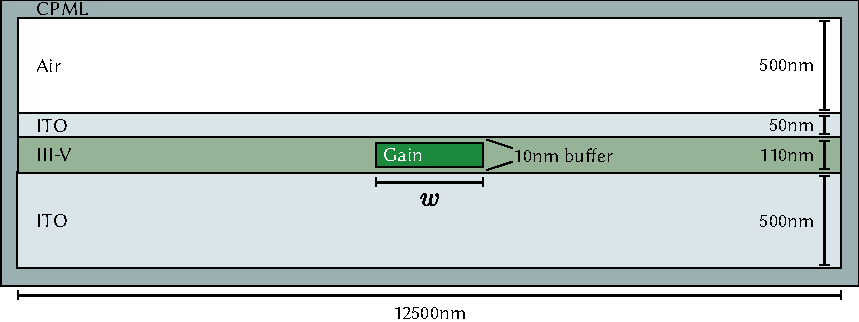
\includegraphics{figs/sl/FdtdScheme.pdf}
 \caption[Schematic of the \fdtd setup]{\label{fig:FdtdScheme}
\textbf{Schematic of the \fdtd setup.}\small\\
The layered structure described in the frequency domain analysis is truncated to
fit in a simulation domain surrounded by \cpml layers.
The pumped gain region is placed in the horizontal centre of the simulation,
and extends a width $w$; vertically it takes up the height of the \threefive layer
that it is embedded in up-to a $10\nm$ buffer on either side.
}
\end{figure}

In this section, the results of and discussions on \fdtd simulations are
presented.
For computational tractability, the simulations presented here are \twod with
uniformity in the $y$ direction.
The layered geometry of \fig{Dispersion} is recreated in these simulations,
with the top and bottom layers (that were unbounded in the analytic study)
having a height of $500\nm$, and the entire structure having a width of
$12500\nm$.
The simulation domain is surrounded with
\emph{convolutional perfectly matched layers} (\cpml) layers,
which quickly attenuate incident fields without introducing reflection such that
they do not interact with the simulation boundary \cite{Roden2000}.
The dielectric layer has a four-level system embedded in it within a region of
width $w$ that varies per simulation in the range $w \in [200, 1500]\nm$,
and a height that is the same height as the host layer with a $10\nm$ buffer on
either side to simulate quenching by the metal layer.
This is depicted in \fig{FdtdScheme} with further simulation parameters that
match the frequency domain analysis as given in \tab{4lvlParams}.

\begin{figure}
 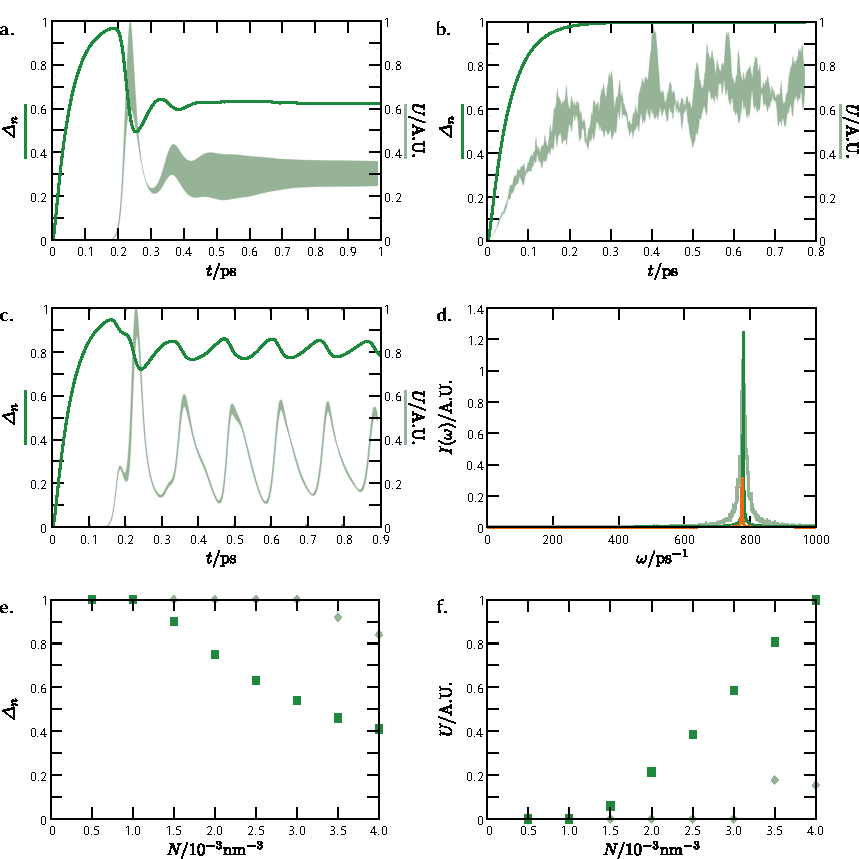
\includegraphics{figs/sl/LasingOnset.pdf}
 \caption[Lasing onset with increasing gain density]{
 \label{fig:LasingOnset}
\textbf{Lasing onset with increasing gain density.}\small\\
\subA, \subB, \subC. Energy density and mean inversion for
\subA. the stopped light structure with a gain density $N=0.002\nm^{-3}$,
\subB. the stopped light structure with a gain density $N=0.001\nm^{-3}$,
\subC. the control structure with a gain density        $N=0.004\nm^{-3}$.
\\
\subD. Power spectra for
\sl structure at $N=0.002\nm^{-3}$ (deep green),
\sl structure at $N=0.001\nm^{-3}$ ($\×5000$ pale green), and
control structure at $N=0.004\nm^{-3}$ (orange).
\\
\subE. Steady state inversion of \sl (deep green) and control (pale green)
structures with varying gain density.
\\
\subF. Steady state cycle averaged energy density with varying gain density.
}
\end{figure}


The first set of simulations examines the general dynamics of emitting into
a stopped light structure.
For a gain region width of $1500\nm$, two sets of simulations are run;
the first with the stopped light structure as described, and the second with a
control structure where the top metal layer has been reduced in thickness
to $20\nm$ with the effect of removing the stopped light points whilst keeping a
\TM1 mode that is in the same frequency range.
In both cases the gain density is varied in a range of $N \in [0.0005,
0.004]\nm^{-3}$.

Of the simulations, the the \sl structure with gain densities above
$N=0.0015\nm^{-3}$ enters a steady state lasing regime after times that vary
between $0.3\ps$ and $0.6\ps$.
Simulations below this density range did not enter into a lasing regime, whereas
there were bursts of \ase, fields never grew strong enough
to lead to sustained lasing.
The control structure also can also enter the lasing regime, albeit requiring
more than double the gain density at $N=0.0035\nm^{-3}$

\FigSub{LasingOnset}{.a-c} plots the mean inversion and energy density of a
point in the centre of the emitter region.
For the cases in the \sl structure that did enter a lasing regime,
characteristic relaxation oscillations can be seen where inversion initially
builds up and spontaneous emission events are induced.
The fields then are amplified as they stimulate further emission, growing the
field in the mode coherently.
From here the emitted fields start to grow exponentially, and when they are of
sufficient strength will deplete the inversion density.
This reduction of inversion feeds back by decreasing the available gain,
leading to a decrease in field energy as the energy in the field is lost to
dissipative processes in the metal layers.
The decrease in energy density allows for the inversion to rebuild.
This continues in an oscillatory manner with the energy density lagging
behind the inversion by 90°.
The amplitude of the inversion and energy oscillations decrease with each
cycle until a stable steady value for both is reached.
In contrast, the control structure, albeit entering a regime of relaxation
oscillations, is more erratic and the oscillations do not settle to a steady
state.
Instead the oscillations continue with a factor of 4 between the peak energy
density and the trough.

Relaxation oscillations are accompanied by a characteristic decrease of the
width of the power spectrum, from a wide peak in \ase,
to a sharp one in the lasing regime, This observation, which is usually taken
as crucial evidence for lasing in experimental setups, is displayed in
\figSub{LasingOnset}{.d}.

For the \sl structure, the inversion density ($N_2-N_1$) needed for lasing is
$0.00148\nm^{-3}$.
If the total density of gain molecules is less than this, then the system
cannot enter a lasing regime, only able to support occasional bursts of
\ase.
Once the lasing threshold has been passed, the energy density in the mode
increases linearly with the gain density.

%Find more things to say here

\subsection{Lasing Mode} \label{sec:lasingMode}

\begin{figure}
 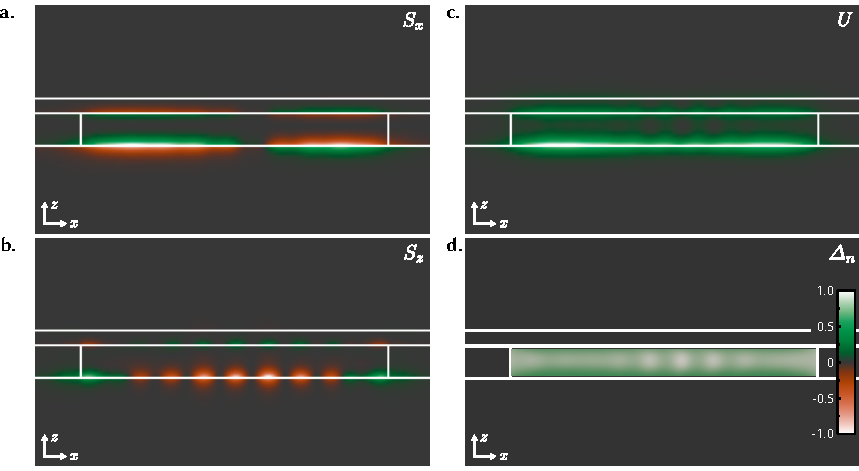
\includegraphics{figs/sl/EnDensPV.pdf}
 \caption[Energy density and flux of lasing mode]{\label{fig:EnDensPV}
\textbf{Energy flux and density of lasing mode.}\small\\
The lasing mode of a \sl structure with a width $1000\nm$.
\subA. and \subB. show the $x$ and $z$ component of the cycle-averaged
Poynting vector respectively, with positive values in green, and negative in
orange.
Focusing on the bottom right lobe of the flux in \subA, energy flows into
the gain region in the dielectric layers and out of it in the metal layer.
For the same lobe in \subB, energy moves downwards out of the gain region
towards the centre, and upwards into the region at the edge.
The counter-clockwise energy vortex in this corner is mirrored in
the other corners.
\\
The cycle-averaged energy density is plotted in \subC. and inversion in
\subD.
The inversion is the complement of the energy density, being highest in areas
with low energy density, and depleted where the mode sits.
}
\end{figure}

In this section, the lasing modes are investigated for \sl structures where
the width of the gain region varies in the range $w \in [200, 1500]\nm$, using a
fixed gain density of $N=0.002\nm^{-3}$.

The spatially resolved, cycle averaged Poynting vector, energy density, and
inversion are plotted in \fig{EnDensPV} for a structure with width $1000\nm$.
The energy is concentrated on metal-dielectric interfaces, strongest on the
lower interface, and is localised around the gain medium despite there
being no cavity along the horizontal direction.

The Poynting vector shows how energy circulates in the structure.
There are four energy flux vortices, one in each corner of the structure, as
described in the figure caption, these have energy move out of the gain region
into the metal layers and into it in dielectric layers.
Considering the $x$ component of the Poynting flux, (\figSub{EnDensPV}{.a}),
the forward and backward flows are in exact balance.
The balanced counter-propagation of energy in the negative-permittivity (metal)
layers against the dielectric layer.
This is the basis of feedback in the system.

The inversion is shown in \figSub{EnDensPV}{.d}, there are areas of spatial hole
burning where the energy density is highest.
The spatial modulation seen is explained when considering the field profile and
its formation.

\begin{figure}
 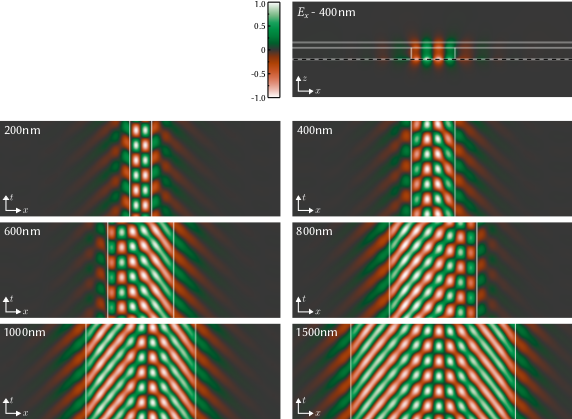
\includegraphics{figs/sl/FieldEvo.pdf}
 \caption[Field evolution in steady state]{\label{fig:FieldEvo}
\textbf{Field evolution in steady state.}\small\\
The $E_x$ field along a line slice at the bottom metal interface is plotted
against time on the vertical axis.
For the $200\nm$ structure, the field inside the gain region is a standing wave.
The other structures have two inward propagating waves which meet at a standing
node.
This node can appear towards the edges, i.e. for $600$ and $800\nm$, or
positioned towards the centre for $1000$ and $1500\nm$.
A stream of plasmons is emitted at either side of the gain region, with a
predominantly negative phase velocity.
}
\end{figure}

It is important to note that the modes that are formed when the structure
enters the lasing regime are a dynamic synthesis of the spectrum of planewave
modes available rather than that of a predefined cavity mode.
The modes that form are propagating waves, with an advancing phase, rather than
purely standing waves, as shown in \fig{FieldEvo}.
It will be shown that this results from modes being centred independently on
finite positive and negative $q$ points, the relative excitation of
each competing with each other, rather than having symmetric excitation at
$q=0$.
This is in contrast even to the stopped light lasing structure considered in
Ref.~\cite{Pickering2014}, which was photonic in nature rather than plasmonic,
and emitted symmetrically about $q=0$ as a standing wave.

In all cases, the modes are inwardly propagating, that is the leftmost half
propagates right and vice versa.
These two halves form a standing wave where they meet, and this node need not be
in the centre of the structure, instead being randomly chosen by the spontaneous
symmetry breaking at the transition from \ase to lasing.
The asymmetry of the mode profile will be discussed later in the chapter.

Lasing is shown to be possible for structures with a gain region width down to
$200\nm$, at which point the steady state inversion rises to around $0.9$.
For this case one observes a standing wave in the gain
interior, i.e. a symmetric excitation of positive and negative $q$ modes.
The confinement of such a structure is at its limit here, with significant
field profile outside the gain region.
For widths smaller than this, there will not be enough gain to pass the lasing
threshold.
This thinnest confinement at $200\nm$ is $12\×$ the free-space wavelength, and
indeed $3.5\×$ the bulk wavelength in the semiconductor layer.

\begin{figure}
 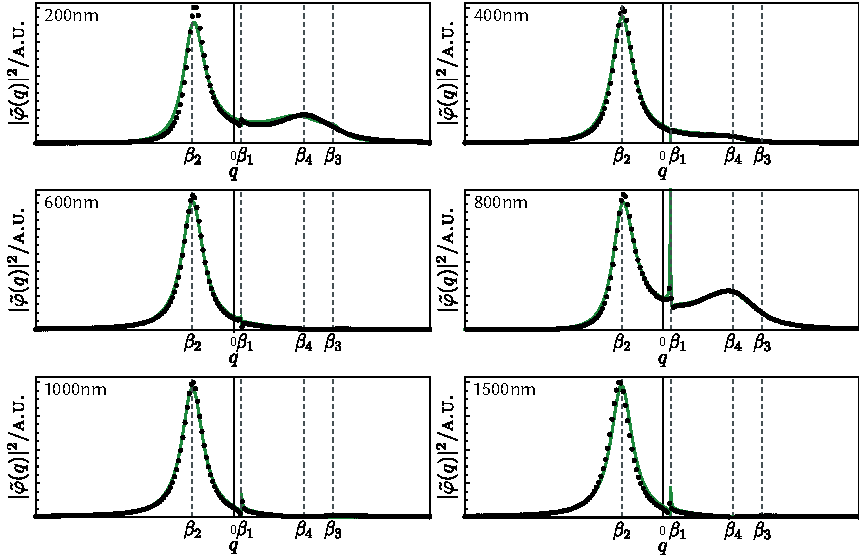
\includegraphics{figs/sl/ComplexQPlasmons.pdf}
 \caption[Complex wavevector plasmons]{\label{fig:ComplexQPlasmons}
\textbf{Complex wavevector plasmons.}\small\\
Power spectra of fields emitted from the right terminal of the gain region
(black dots).
This is fit to the lineshape of the first four \cwv plasmons (green line), i.e.
a Lorentzian function, $|\tilde\φ(q)|^2 = |\sum_i^4\φ_i / (q-\β_i)|^2$.
The amplitudes are varied to fit, but the wavevectors are fixed from the
\cwv plasmon dispersion at the lasing frequency (See \tab{slprops}).
The imaginary part becoming the width in the spectral density.
In each, the negative phase velocity $\β_2$ plasmon is strongest,
with $\β_4$ having a large amplitude for $200\nm$ and $800\nm$ which can be also
seen in the field profiles of \fig{FieldEvo}.
}
\end{figure}

Outside of the gain region, a stream of plasmons is emitted to either side
with a negative phase velocity.
For these plasmons, it makes sense to use a complex-wavevector picture to
describe them, as we have a steady state oscillating source, for which the field
is known at a fixed point in space (the edges of the gain region), for which we
wish to consider the spatial evolution away from this point.

One can analyse the spectral content of the fields, once the system has
entered into a steady state.
Using \emph{discrete Fourier transform} (\fft) methods, the peak frequency
component, $\ωpeak$, of the electric field is identified and isolated.
This returns a spatially resolved, complex valued function $\Etilde(\x,
\ωpeak)$.
Taking a spatial Fourier transform along the waveguide ($x$) axis, allows the
extraction of the spatial power spectrum, which is averaged over $z$ positions
within the gain layer, $I(q) = |\Etilde(q, \ωpeak)|^2$.

The wavevector of the emitted plasmon can be extracted by taking the \fft over
positions outside of the emitting gain region.
\Fig{ComplexQPlasmons} shows the spectrum of fields emitted from the right
terminal, i.e. integrating from the edge of the gain region up to but excluding
the \cpml layer.
These data are fit to the first four analytically determined complex-wavevector
modes (see \fig{Dispersion}) at the lasing frequency.
The wavefunction of such modes is the Fourier transform of a complex decaying
exponential,
\begin{subequations}\subeq
\begin{align}
\φ(x) &= \θ(x)\exp(i \Re \β_i \, x)\exp(-\Im \β_i \, x) \\
\tilde{\φ}(q) &\propto \frac{1}{q-\β_i}
\;,
\end{align}
\end{subequations}
where $\β_i$ is the complex wavevector of the bound mode \spp.
This is summed over each of the first four plasmons, each with a complex
amplitude, then the absolute square of this is compared with the data, i.e.
\begin{equation}
|\φ(q)|^2 = \left| \sum_{i=1}^4 \frac{\φ_i}{q-\β_i} \right|^2
\;.
\end{equation}
The fit allows the amplitude of each resonance to change, but keeps
the wavevectors constant.
Excellent agreement is found, confirming the presence and applicability of the
description of complex-wavevector plasmons.

The negative group velocity plasmon $\β_2$, has the strongest amplitude in all
cases, though the narrow width $\β_1$ plasmon is present too.
In cases where the standing wave node is close to the terminal, i.e. for $w =
200, 400, 800\nm$ there is significant excitation of the short propagation
length $\β_4$ plasmon.

Thus, stopped light lasing can be utilised as a source of coherent plasmons at a
single frequency and discrete wavevector.
Alternatively by adding a grating to the structure away from the gain region,
the plasmons may be outcoupled, converting this into a photonic \sl laser.

\begin{figure}
 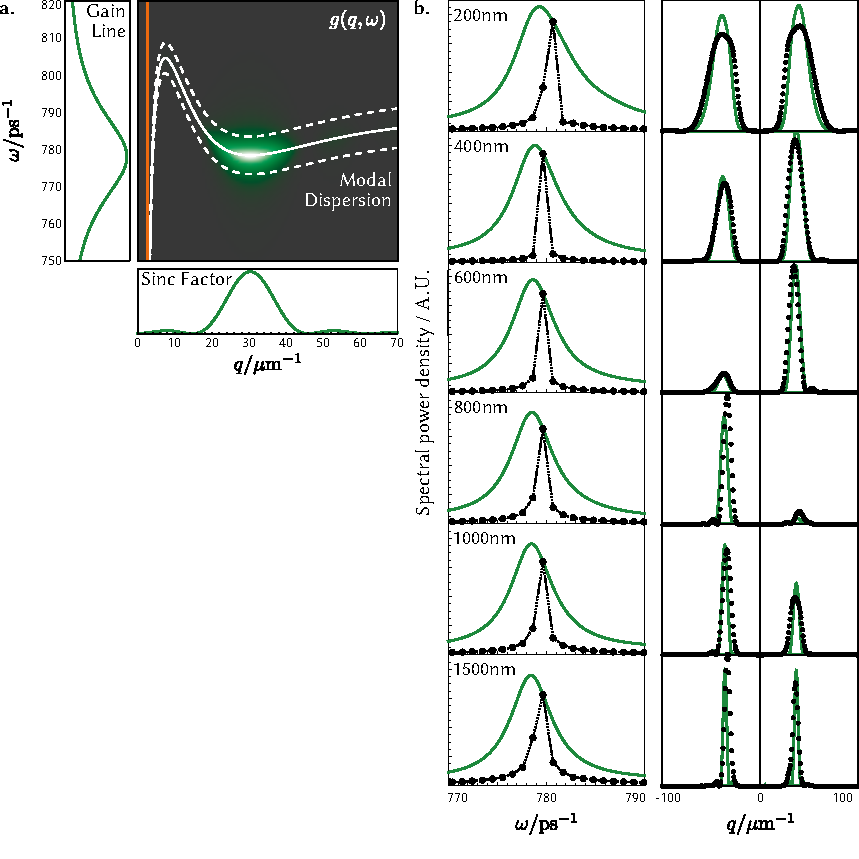
\includegraphics{figs/sl/ModeShape.pdf}
 \caption[Power spectrum of lasing modes]{\label{fig:ModeShape}
\textbf{Power spectrum of lasing modes.}\small\\
\subA. Coupling strength $g(q,\ω)$, which is composed of the
emission lineshape (left), the \emph{sinc} function of the gain region (bottom),
and the mode support (overlayed).
The frequency which maximises the the integral of $g$ over wavevector is
\emph{picked} by the system to lase at. \\
\subB. temporal and spatial power spectrum of the lasing mode for model (green
lines) and \fdtd data (black points).
The spatial mode profile is modelled by a modified form of the coupling strength
at the lasing frequency, as given by \eq{lasingShape}.
Results are in excellent agreement with the \fdtd results.
}
\end{figure}

The spatial power spectrum, $I(q)$, can also be taken over the entire domain,
rather than in the interval to the right of the gain region, in order to
capture the profile of the lasing mode.
This function is not symmetric about $q=0$ since it was transformed
from a complex valued function.
Hence it does not follow the usual evenness
properties of the Fourier transform of a real function.
This allows for inspection of how the positive and negative wavevector (and
hence phase velocity) modes are independently excited.
\FigSub{ModeShape}{c} plots the power spectra of lasing modes in the range of
gain widths considered.
It can be seen that in each case, the power spectrum is a bimodal distribution
with peaks about $q \approx \pm 30.7\μm^{-1}$, which is exactly the wavevector
of the second stopped light point.
As one would expect, the width of each peak is inversely proportional to the
gain width chosen, e.g. the smallest gain section at $200\nm$, the width is
around $5\μm^{-1}$.
There is no preferential excitation of the peaks, and
seemingly no correlation between their relative amplitude.
This is because they are two competing modes, one of which will initially
take the lead in growth due to the spontaneous symmetry breaking of amplified
spontaneous emission.
The first mode will dominate the gain, being able to exponentially grow in field
strength.
The second mode may still be allowed to grow but spatially separated from the
first, harvesting areas where the field and gain are less strongly coupled.
This picture is corroborated when viewing the time evolution of the steady state
fields, which show two lobes, inward propagating, with a finite overlap width
where the wave becomes standing, this is depicted in \fig{FieldEvo}.
This is developed further in Ref.~\cite{Wuestner2015}, where it is shown how the
location of the nodes move on longer time scales.

It is possible to predict the spectral content of the lasing mode.
Plasmons are emitted into the frequency which maximises the effective
gain,
\begin{subequations}\subeq
\begin{align}
G(\ω) &=
\int_{-\infty}^{\infty}\d{q} \:
g(q, \ω)
\\
g(q,\ω) &=
\frac{\γL / \π}{(\ω-\ωL)^2 + \γL^2}
\frac{\γpl(q) / \π}{(\ω-\ωpl(q))^2 + \γpl(q)^2}
\sinc^2 \left( \frac{w (q - q_2)}{2} \right)
\,.
\end{align}
\end{subequations}
This expression is the product of three terms;
firstly, there is the emission lineshape of the gain medium,
this is multiplied by the density of states of bound modes that are available to
emit into.
The final part is a geometrical factor, that is the square of the Fourier
transform of a “tophat” function of width $w$, which represents the width of the
gain area.
There can be modulation of the emitted field in the gain region, so the sinc is
allowed to be translated in $q$-space, and will centre itself at the
\zgv2 point $q_2$.
\Fig{ModeShape} shows the frequencies that maximise the effective gain and the
frequency range that was emitted at in the simulations.
This is presented alongside a the coupling strength $g(q,\ω)$ for a $400\nm$
gain section.
This frequency of highest gain can then further be used to predict the mode
shape $I(q)$, up to a factor of the weights of the mode in the $+q$ and $-q$
excitation ($I^+, I^-$),
by a slight modification of $g(q,\ω)$, to include both excitations,
\begin{equation} \label{eq:lasingShape}
I(q) \propto
\frac{\γpl(q)}{(\ω-\ωpl(q))^2 + \γpl(q)^2}
\left(
I^+ \sinc \left( \frac{w (q - q_2)}{2} \right) +
I^- \sinc \left( \frac{w (q + q_2)}{2} \right)
\right)^2
\;,
\end{equation}
which is in excellent agreement with the \fdtd spectra.

\section{Conclusions} \label{sec:slConc}
This chapter has introduced
\emph{plasmonic stopped light lasing}, whereby plasmons are localised by
reducing the group velocity of a wavepacket to zero whilst within a gain medium.
This is in contrast to traditional nanolasing schemes, which localise energy
in a resonant cavity.

In order to explain the concept, topics of dispersion, and the
nuances of the complex-frequency/complex-wavevector pictures have been
discussed.
Frequency domain methods have been employed alongside an evolutionary
optimisation algorithm in order to characterise the properties and quality of a
structure and select for optimal structures within constraints.

An exemplary structure was introduced, composed of realistic
materials, whose properties were studied throughout the rest of the chapter.
Analysis in frequency domain was continued to investigate how, in the small
signal gain regime, a two-level emitting resonator could compensate for the
inherent material losses in metal layers, determining idealised threshold
values of inversion required to free a mode of damping.

Equipped with this analysis, finite difference time domain simulations were made
of the test structure, in order to capture the dynamics of spatial and nonlinear
effects.
The previous frequency domain analysis of the threshold inversion was
corroborated by varying the gain density in each time domain simulation, and it
was found that lasing is indeed possible in this scheme.

The lasing mode was investigated, and a model for predicting its modal content
proposed.
It was found that the feedback provided from stopped light lasing ultimately
derives from a dynamically formed vortex of power flow, with propagation and
counter-propagation balancing between the dielectric and metal layers.
Despite being stopped, the lasing mode carries a finite phase velocity, with an
inward propagating phase modulation that can be detected from the top of the
structure.

As an output of the lasing process, coherent plasmon polaritons (sitting on the
cusp of the complex-wavevector dispersion curve) are emitted from the sides of
the gain region.

This is a new type of subwavelength laser, where the active component is
smaller than a few hundred nanometres, and coherently emits plasmons directly
into a waveguide without relying on external coupling mechanisms.
The dynamic formation of the cavity-free lasing mode is a new physical feature,
the implications of which are open.
It could become the basis for single frequency coherent \spp generation in
quantum plasmonic applications \cite{Jacob2011,Tame2013}, or as the basis of a
quantum fluid such as a photonic Bose-Einstein Condensate \cite{Carusotto2013}.

\begin{table}
 \begin{tabular}{ c | l r l} 
  Symbol	& Parameter 							& Value \\ \hline
  $\εinf$	& Drude high frequency permittivity		& $4.0$		& \\
  $\ωp$		& Drude plasma frequency				& $3130$	& $\ps^{-1}$ \\
  $\γp$		& Drude loss							& $10.7$	& $\ps^{-1}$ \\
  \hline
  $\εbg$	& Background permittivity				& $11.68$	& \\
  $\ωe$		& Emission frequency					& $778$		& $\ps^{-1}$ \\
  $\γe$		& Emission width						& $31.7$	& $\ps^{-1}$ \\
  $\σe$		& Emission cross section		& $\sci{2.12}{-7}$	& $\μm^2$ \\
  $N$		& Carrier density					& $\sci{2}{6}$	& $\μm^{-3}$ \\
  \hline
  $\τ_{10}^{-1}$	& Non-radiative decay rate (0→1)& $10$	& $\ps^{-1}$ \\
  $\τ_{21}^{-1}$ & Non-radiative decay rate (1→2)& $0.002$	& $\ps^{-1}$ \\
  $\τ_{32}^{-1}$	& Non-radiative decay rate (2→3)& $10$	& $\ps^{-1}$ \\
  $\rp$				& Electrical pump rate (0→3)	&  $1$	& $\ps^{-1}$ \\
  \hline
 \end{tabular}
 \caption[Simulation parameters]{\label{tab:4lvlParams}
\textbf{Simulation parameters.}\small\\
Parameters for frequency domain and \fdtd simulations,
divided into:
metal Drude model,
emitter Drude-Lorentz parameters,
\fdtd four-level system parameters.
}
\end{table}

\begin{table}
 \begin{tabular}{ c | l r l} 
  Symbol	& Parameter 						& Value \\ \hline
  $d_1$	& \threefive layer thickness			& $0.110$	& $\μm$ \\
  $d_1$	& \ito layer thickness					& $0.050$	& $\μm$ \\
  \hline
  $q_1$	& \zgv1 wavevector						& $7.41$	& $ \μm^{-1} $ \\
  $\ω_1$	& \zgv1 frequency			& $805 + \i\,4.14$	& $ \ps^{-1} $ \\
  $q_2$	& \zgv2 wavevector						& $30.3$	& $ \μm^{-1} $ \\
  $\ω_2$	& \zgv2 frequency			& $778 + \i\,5.06$	& $ \ps^{-1} $ \\
  \hline
  $\Δq$	& wavevector bandwidth					& $22.9$	& $ \μm^{-1} $ \\
  $\Δω$	& frequency bandwidth					& $26.3$	& $ \ps^{-1} $ \\
  $\vb$	& band velocity							& $1/262$	& $ \c $ \\
  \hline
  $\β_1$	& \cwv mode 1	& $3.94 + \i\,0.131$	& $ \μm^{-1} $ \\
  $\β_2$	& \cwv mode 2	& $-21.3 + \i\,6.71$	& $ \μm^{-1} $ \\
  $\β_3$	& \cwv mode 3	& $51.2 + \i\,6.53$		& $ \μm^{-1} $ \\
  $\β_4$	& \cwv mode 4	& $36.1 + \i\,16.1$		& $ \μm^{-1} $ \\
  			& \cwv frequency			& $778$		& $ \ps^{-1} $ \\
  \hline
 \end{tabular}
 \caption[Properties of optimised \sl structure]{\label{tab:slprops}
\textbf{Properties of optimised \sl structure.}\small\\
Divided into:
Thicknesses of material layers,
coordinates of \zgv points in the dispersion relation,
band metrics,
complex wavevector modes at the \fdtd emission frequency.
}
\end{table}
 % Chapter 3 - Stopped Light
\clearpage~\clearpage
\chapter{Active Plasmons in Nonequilibrium Graphene}

\section{Introduction} \label{sec:grIntro}

\begin{figure}
 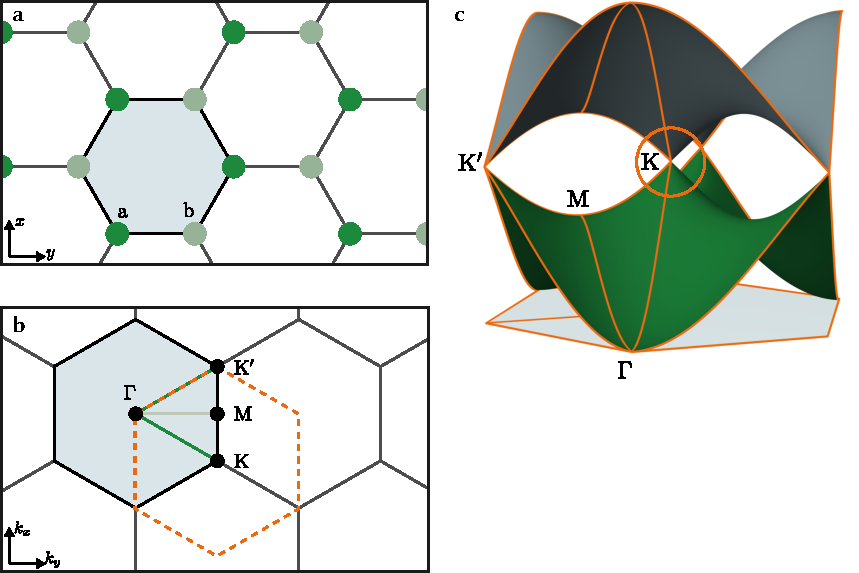
\includegraphics{figs/gr/TB.pdf}
 \caption[Graphene structure and tight binding model]{
\label{fig:Tb} \textbf{Graphene structure and tight binding model.}\small\\
\subA. Graphene's molecular structure, composed of two overlapping triangular
sublattices of $\mathrm{a}$ and $\mathrm{b}$ sites.
The hexagonal unit cell is shaded.
\\
\subB. Reciprocal space lattice, marking points of high symmetry
($\Gamma, \mathrm{M}, \mathrm{K}, \mathrm{K'}$).
The 1\st Brillouin zone is shaded, and the Wigner-Seitz cell about the
$\mathrm{K}$ point is highlighted.
\\
\subC. Tight binding electron dispersion about the $\mathrm{K}$ point.
The fully occupied valence band is shown in green, and empty conduction band in
black.
The dispersion relation is conical in the immediate vicinity of the
$\mathrm{K}$ point (and equivalently about the $\mathrm{K'}$ point).
}
\end{figure}

Graphene has gained widespread scientific interest since 2004
\cite{Allen2010,Schwierz2010,Sanchez2012,Cooper2012,Pumera2013}
when it was shown that it could be experimentally produced by exfoliating a
single layer from graphite \cite{Novoselov2004}.
It is a \twod crystal of carbon, where the atoms are arranged in a flat
hexagonal tiling, with σ-bonds binding each atom to its three nearest
neighbours.
Each atom has a remaining $2\mathrm{p}_z$ orbital which contributes to the
bonding by overlapping with its nearest neighbours forming a half-filled π-band
\cite{CastroNeto2009}.
The π-band can be modelled in a tight-binding formalism, which transforms
orbitals of electrons sitting at one of the atomic sites, $\mathrm{a}$ or
$\mathrm{b}$, into energy eigenstate planewaves in the conduction and
valence band.
The tight binding band structure is shown in \fig{Tb} about the $\mathrm{K}$
symmetry point, alongside diagrams of the lattice in real and reciprocal space.
About this point, the dispersion relation of electrons is linear and the two
bands meet with a vanishing energy gap, forming what is known as the
\emph{Dirac cone} since the electrons that sit there may be described
by a relativistic Dirac equation.
The equation describes massless particles with a “speed of light” given by
the Fermi-velocity $\vF \approx c / 300$ lending them the name
\emph{massless Dirac fermions} (\mdfs).

It is graphene's properties as a \twod metallic material with a linear dispersion
and zero bandgap that give it remarkable electronic and optical properties
\cite{Novoselov2005,Avouris2007,CastroNeto2009,Bonaccorso2010,DasSarma2011},
%such as
%large intrinsic carrier mobilities \cite{},
%electric field effect \cite{Novoselov2004}, and
It also allows for a strong optical interaction with the \mdf plasma in both a
linear \cite{Falkovsky2007a,Kuzmenko2008,Nair2008,Mak2008}
and nonlinear regime
\cite{Mikhailov2007a,Hendry2010,Ishikawa2010,Nesterov2013}.
Though perhaps one of graphene's most useful properties is its tunability;
the Fermi-level of graphene can be set by chemical doping 
or a gate voltage \cite{Kim2010,Liu2011a,Ju2011,Fei2012}.
Coupled with a conical dispersion up to energies of $\sim\!1\eV$, this allows
broadband optical operation in the visible and infrared.
This has been exploited for the construction of nanoscale devices such as
photodetectors \cite{Mueller2010,Withers2013,Liu2014},
modulators \cite{Liu2011},
saturable absorbers \cite{Bao2009},
metamaterial devices \cite{Lee2012,Vakil2012,Hamm2013},
and for use in sensing applications \cite{Schedin2010,Lee2012a}.

The aspect of graphene that will be primarily focused on in this thesis it its
ability to support plasmons
\cite{Shin2011,Chen2012,Fei2012,Grigorenko2012,Bao2012,Low2014,Stauber2014,
GarciaDeAbajo2014,Agarwal2015}.
The coupling of these charge density waves to the electromagnetic field allows
for confinements that are on the order of $1/100$ of the free-space wavelength
\cite{Koppens2011,Chen2012}.
Plasmons appear as the poles of the Coulomb potential, calculated from the
dynamic polarisation in the \emph{random phase approximation} (\rpa)
\cite{Wunsch2006,Hwang2007}.
%some more about plasmons

Despite having a high conductance, plasmons on doped graphene have high losses
resulting in propagation lengths that are typically smaller than the wavelength
\cite{Tassin2012}.
This is due to Landau damping; the generation of electron hole pairs by the
absorption of plasmons, as well as collisional damping channels
\cite{Yan2013,Low2014}.
Much like in metal plasmonics, graphene's utility as a plasmonic platform will
rely on being able to mitigate these losses.

The semimetal properties can be utilised to this end.
Exciting graphene with a short optical pulse will generate hot electron/hole
pairs.
These carriers quickly relax via intraband processes within their respective
band but are subject to a bottleneck for interband recombination processes
which leads to the formation of a quasiequilibrium of inverted carriers
yielding optical gain \cite{Ryzhii2007,Li2012,Winzer2013}.
This gain is also available to plasmons which may be amplified by stimulated
emission \cite{Rana2008,Rana2011,Dubinov2011,Popov2012} enhanced by the tight
confinement of plasmons on the graphene sheet.

The balance of absorption and emission rates in graphene, and hence the presence
of net gain, is critically dependent on the exact form of the plasmon dispersion
relation.
Previous studies have considered this in approximative form, rather than as the
exact complex solution to the \rpa polarisability.
It therefore remains to be seen whether under conditions of inversion, finite
temperature, collision loss, and doping, plasmons indeed exist and can become
undamped.

Stimulated emission in a system is always accompanied by spontaneous emission
where carrier pairs spontaneously recombine emitting broadband incoherent
photons \cite{Mecklenburg2010} and plasmons.
The enhanced field of the plasmon modes and low group velocity gives rise to a
high density of optical states, thereby accelerating the spontaneous emission
rate from an equivalent dipole transition in free space \cite{Nikitin2013}.

From the point of view of the carrier system, spontaneous recombination
by plasmon emission represents an ultrafast relaxation channel
\cite{Bostwick2007,George2008,Rana2011} that may indeed play a primary role in
the dynamics of hot carrier relaxation
\cite{Girdhar2011,Malic2011,Kim2011,Winzer2012,Sun2012,Tomadin2013,Sun2013}.
This is a process that has often been attributed to
\emph{Auger recombination} (\ar) \cite{Brida2013, Breusing2011},
part of a family of Auger processes,
which are two-body Coulombic carrier-carrier scattering processes that include
\ar, impact ionisation, inter- and intraband scattering \cite{Tomadin2013}.
The particular role of this channel however is subject to discussion, as the
collinear Auger processes are suppressed when considering dynamic screening in \rpa
\cite{Tomadin2013, Tielrooij2013}.

The timescales for carrier recombination emitting plasmons have been reported to
vary between $10\fs$ and $100\ps$ in first theoretical studies
\cite{Bostwick2007,George2008} therefore accurate determination of the
timescales is key to establish the primacy of plasmons as a channel for
inversion decay.

Experimentally, the relaxation of hot carriers has been observed in
\emph{time resolved, angle resolved photo-emission spectroscopy} (\trarpes)
\cite{Bostwick2007,Gierz2013,Johannsen2013,Gierz2014,Gierz2015},
and pump-probe setups
\cite{Dawlaty2008,Choi2009,Breusing2009,Breusing2011,Sun2012,Li2012,Malard2013,
Jensen2014},
and has shown thermalisation within the bands at a timescale of $10\fs$ and
interband recombination decaying the inversion over $\sim100\fs$. 

Whereas the polarisability, and derived plasmons, have been studied extensively
in the case of a thermal equilibrium of doped Graphene
\cite{Vafek2006,Wunsch2006,Hwang2007,Mikhailov2007,Wang2007,Pyatkovskiy2009,
Ramezanali2009,Jablan2009,Scholz2011,Scholz2012,Gutierrez-Rubio2013},
there has so far not been a general formalism for calculating complex valued
polarisabilities for nonequilibrium carrier distributions.

\subsection{Organisation of chapter}
This chapter will start in \sec{graphenePol} by introducing the zero-temperature
equilibrium polarisability of graphene, which will provide the basis in later
sections for more generalised polarisabilities.
The complex frequency plasmon dispersion will be presented, which exactly solves
the \rpa dielectric function, and compared to approximative schemes.

Next in \sec{NEPol}, a method to generalise the plasmon dispersion to arbitrary
isotropic carrier distributions will be derived.
This will be assisted by the introduction of scale-free variables,
which sets all quantities relative to the tunable Fermi-level.

The quasiequilibrium polarisability will be presented in \sec{quasieq}
which describes photoinverted carriers that have
thermalised within their respective bands.
The plasmon dispersion of photoinverted graphene is calculated from the new
polarisability expression, for both intrinsic and doped graphene, showing that
plasmons with gain are indeed possible in an idealised case.

Improvements are made to the model in \sec{coltemp}, to include the effects
of collision loss and finite temperature, which will both reduce the gain
available to plasmons.
The calculation for temperature presented in this section works for low
temperatures, but will be shown to break down as $T$ increases.
This will be remedied in \sec{hotCarriers}, where it is explicitly shown how to
calculate the polarisability for arbitrary carrier distributions using a
contour integral method.
This allows for the evaluation of polarisabilities with high temperature
Fermi distributions, but also that of a non-Fermi distribution of hot
photoexcited graphene.

\Sec{sponEmit} calculates the spontaneous emission of photoinverted graphene,
and the associated carrier recombination rates. This is done exactly at zero
temperature, and with a Fermi's golden rule scheme for cases of collision loss
and finite temperature, with an accuracy that is dependant on using the exact
complex frequency plasmon dispersion.

Finally in \sec{npe}, the inversion decay dynamics of the carrier system are
considered with nonequilibrium plasmons emission as the channel for spontaneous
recombination.

\section{Plasmon Modes of Equilibrium Graphene} \label{sec:graphenePol}
In a similar manner to the surface of a metal, \twod materials endowed with
charge carriers, such as graphene, may support surface plasmon modes.
One of the main differences though notes is that there is no bulk medium
unlike for metal plasmons, and the charges are entirely confined to the \twod
sheet.
This means that the presence of modes relies solely on the characteristic of
the surface conductivity $\σs$, rather than the bulk properties of a conducting
substrate.

Graphene, in contrast to metals, supports two types of collective plasmon
excitations, labelled by their electromagnetic field configuration; the
transverse magnetic (\TM) modes that are associated with the longitudinal
density-density response of the \mdf plasma
\cite{Wunsch2006,Principi2009,Stauber2010a,Pellegrino2011,Gutierrez-Rubio2013},
and have similar field characteristics as their metal counterpart; and
transverse electric (\TE) modes associated with the transverse current-current
response and have no metal counterpart.
T\textsc{e} plasmons only exist in a limited frequency range and are weakly
bound \cite{Gutierrez-Rubio2013}, as such, only the \TM plasmons are considered
in this thesis as they are strongly coupled to the \mdf plasma
\cite{Polini2008,Bostwick2010}.

%and thus constitute the dominant channel for stimulated and spontaneous
%emission \cite{Nikitin2011a,Stauber2012a}

The dispersion relation of the \TM mode can be solved using the transfer matrix
method formalism of \sec{introTMM}.
Assuming a conducting sheet sandwiched between two (isotropic, non-magnetic)
semi-infinite half-spaces, the transfer matrix is,
\begin{subequations}\subeq
\begin{equation}
\Mtr = \v{U}^{-1}_\sup  \v{S}  \v{U}_\sub
\;,
\end{equation}
or in full,
\begin{equation}
\Mtr =
\frac{1}{2}
\begin{pmatrix}
  1 & Z_\sup \\
  1 & -Z_\sup
\end{pmatrix}
\begin{pmatrix}
  1 & 0 \\
  -\Zf \σs & 1
\end{pmatrix}
\begin{pmatrix}
  1 & 1 \\
  1/Z_\sub & 1/Z_\sub
\end{pmatrix}
\;,
\end{equation}
\end{subequations}
yielding the condition for the presence of bound modes as,
\begin{equation}
\frac{1}{Z_\sub} + \frac{1}{Z_\sup} + \Zf\σs = 0
\end{equation}
which, for \TM modes is,
\begin{equation}
\frac{\εpar_\sub}{\sqrt{q^{2} - \εpar_\sub (\ω/\c)^2}} +
\frac{\εpar_\sup}{\sqrt{q^{2} - \εpar_\sup (\ω/\c)^2}} +
\frac{\i \c}{\ω} \Zf \σs
= 0
\;.
\end{equation}
Neglecting wave retardation, i.e. $q \gg \ω / \c$, and by defining
$\εbar = (\εpar_\sub + \εpar_\sup)/2$,
one may cast this into a simplified form
\cite{Stern1967,Mikhailov2007,Jablan2009},
\begin{equation}\label{eq:dispConduct}
1 + \frac{\i q}{2 \εbar \εf \ω} \σs(\q, \ω) = 0
\;,
\end{equation}
here $\σs(\q, \ω)$ is the nonlocal sheet conductivity, i.e. the linear
electronic response to a monochromatic electromagnetic planewave.

\Eq{dispConduct} will have solutions for a conductivity with positive
imaginary part.
The particular functional form of the conductivity will determine the
characteristics of the plasmon solutions.

The plasmon may also be solved for in linear response theory of
collective charge oscillations of a \twod electron gas
\cite{giuliani2005quantum}.
In the \emph{random phase approximation} (\rpa), the plasmon dispersion is
determined from the roots of the dielectric function
\cite{Hasegawa1969,bruus2004many},
\begin{equation}\label{eq:εRPA}
\εRPA \coloneqq 1 - V_q \Π(\q, \ω) = 0
\;,
\end{equation}
where $V_q = {e^2} / {2 \εbar \εf q}$ is the bare \twod Coulomb potential in
reciprocal space and $\Π(\q, \ω)$ is the irreducible polarisability, which is
the Feynman propagator of electron-hole pairs \cite{Abergel2010}.
Both $\Π$ and $\σs$ represent linear responses, so \eqs{dispConduct}{εRPA} can
be directly compared giving the relationship between the sheet conductivity and
polarisability in \rpa as,
\begin{equation} \label{eq:condpol}
\σs(\q,\ω) = \i e^2 \ω / q^2 \Π(\q,\ω)
\;,
\end{equation}
noting that the \rpa has been shown to be surprisingly accurate for graphene
\cite{Hofmann2014}.

The plasmon dispersion is defined by the zeroes of the dielectric function,
which in general is a complex-valued function of complex variables.
These zeros may be found for either a real-wavevector/complex-frequency or
real-frequency/complex-wavevector, and it is the former that is
considered here.
That is solutions characterised by a real wavevector eigenvalue, $q$, with
the imaginary part of the frequency representing a decay rate of plasmons over
time.
The exact solution to this equation, the \emph{complex frequency plasmon
dispersion} (\cfpd), is sought within this chapter.

%Assuming a weakly interacting 2D electron gas, the irreducible
%polarizability is, in random-phase approximation (RPA), replaced by
%the leading order term. We note that the RPA is a commonly employed (see
%e.g.~ref.~\cite{Hwang2007})


\subsection{Complex Frequency Plasmon Dispersion} \label{sec:cfpd}
A major objective of this work is to characterise the gain and absorption
spectra of graphene under a variety of electronic configurations.
Plasmons in graphene will couple strongly to the electron-hole plasma,
interacting via single-particle excitation processes: spontaneous emission,
stimulated emission, and stimulated absorption.
The imaginary part of the frequency of the plasmon dispersion encodes the net
stimulated absorption/emission rate and therefore to get a handle on this,
the \cfpd should be solved for exactly within the \rpa framework.
Previously in the literature, the plasmon dispersion has been solved for in a
low-loss approximation for zero temperature equilibrium graphene
\cite{Wunsch2006,Hwang2007}.

The basis for calculations involving the polarisability\footnote{
Or strictly speaking, its leading order term.}
in \rpa is the Lindhard formula
\cite{Stern1967,Wunsch2006,Hwang2007,Wang2007} given as a functional of the, in
general nonequilibrium, electron distribution $n(\έ)$,
\begin{equation}\label{eq:lindhard}
\Π[n](\q,\ω) = \frac{g}{A} \sum_{s,s'=\pm} \sum_{\k}
M^{s s'}_{\k,\k+\q}
\frac{n(\έ^s_{\k}) - n(\έ^{s'}_{\k+\q})}
{\έ^s_{\k} - \έ^{s'}_{\k+\q} + \ħ\ω + \i\times0}
\;.
\end{equation}
The polarisability describes the noninteracting (unscreened) response of the
\mdf plasma to external density perturbations.
Contained within is a sum over all possible transitions $(\k,s) \→ (\k + \q,
s')$, for each initial and final band $s, s' \in \{+,-\}$, at the given wavevector and frequency for a particular
particle/hole distribution $n(\έ)$.
The sum is weighted by the transition matrix element
$M^{s s'}_{\k,\k+\q}$, a quantity determined by the tight binding model that
encodes the honeycomb geometry of Graphene, with the value,
$M^{s s'}_{\k,\k+\q} = [1 + s s' \cos(\θ_{\k,\k+\q})] / 2$
\cite{Kotov2012}.
The Lindhard formula sums over degenerate spin and valley (about $\mathrm{K}$
and $\mathrm{K'}$ points) transitions, leading to the prefactor $g=4$.
In the \mdf approximation, the electronic band dispersion is conical in the
near vicinity of the Dirac points, i.e. $\έ^s_{\k} = s \ħ\vF|\k|$.

Closed form and semi-analytical solutions to the Lindhard formula have been
presented in the literature for the case of graphene in thermal equilibrium,
i.e. for the electronic configuration taking the form of a Fermi-distribution,
\begin{equation}
n(\έ) = f(\έ - \μ, T) = \frac{1}{1 + \exp \big( (\έ - \μ)/\kB T \big) }
\;.
\end{equation}
In the limit of zero temperatures the Fermi function reduces to a Heaviside step
function, $f(\έ - \μ, T=0) = \θ(\μ - \έ)$,
and solutions to this have been first presented for real valued dynamic
variables $(\q,\ω)$ in piecewise form in Refs.~\cite{Wunsch2006,Hwang2007}.
Similarly, later temperature semi-analytical form for real variables has
been derived \cite{Ramezanali2009}.

Assuming a real valued wavevector that acts as the modal eigenvalue,
the plasmon dispersion can be solved by finding the zeros of the dielectric
function \eq{εRPA} for a complex frequency
$\εRPA \big( q, \ωpl(q) - \i \γpl(q) \big) = 0$.
The sign convention of $\γpl$ has been chosen such that it represents a
decay rate for positive values, and amplification due to stimulated emission
when $\γpl < 0$.
If the plasmon couples to single particle excitations, giving it a finite
lifetime, then the frequency does indeed become complex and
the dispersion becomes insoluble with formalisms that are only functions of real
variables, i.e. containing Heaviside step functions.

For cases where the loss is small, $\γpl \ll \ωpl$, a first order
approximation is often used to solve for the real part of the frequency using
just the real part of the dielectric function,
\begin{subequations}\subeq \label{eq:lowloss}
\begin{equation}
\Re \εRPA(\ωpl, q) \approx 0
\;,
\end{equation}
then the imaginary part is given as\footnote{ Or equivalently as
$\γpl \approx {\Im \Π(\ωpl, q)} \big/ {\Re
\left.\pd{\Π}{\ω}\right|_{\ω = \ωpl}}$.
}
\cite{Pyatkovskiy2009,fetter2012quantum,Principi2013},
\begin{equation}
\γpl \approx {\Im \εRPA(\ωpl, q)} \bigg/ {\Re
\left.\pd{\εRPA}{\ω}\right|_{\ω = \ωpl}}
\;.
\end{equation}
\end{subequations}
In regimes where $\Im \εRPA(\ωpl, q) = 0$ then the above equations
become exact, i.e. $\γpl = 0$, which is the case for quasi-loss-free regimes
where there is no Landau damping (absorption or emission).

The polarisability becomes singular for $\ω \→ \vF q$, which means that
solutions of \eq{lowloss} (for real $\ωpl$) can not cross the Fermi line into
the region of intraband excitations as $\Π(q,\ωpl(q)) \→ \infty$ and \eq{εRPA}
can never hold anywhere on the line.
There may exist, and indeed do, complex solutions which do cross the Fermi line,
making this low-loss approximation only appropriate for small wavevectors away
from $\ω = \vF q$.

In order to present an accurate analysis of the single particle excitation processes in
graphene the \cfpd must be solved for exactly, first in the equilibrium
case and subsequently in general for arbitrary nonequilibrium electronic
distributions.

In Ref.~\cite{Pyatkovskiy2009} an analytic expression for the polarisability is
presented, which subject to a change of unit convention and some refactoring, is
given as,
\begin{subequations}\subeq\label{eq:analPolar}
\begin{align}
\Π^{\T=0}_{\μ}(\q,\ω) &\coloneqq \Π[\f(\έ-\μ, \T=0)](\q,\ω)
\\
&= \frac{g\μ}{8 \π \ħ^2 \vF^2} \Πtil_1
\left( \frac{\ħ\vF\q}{\μ},\frac{\ħ\ω}{\μ} \right)
\;,
\end{align}
where,
\begin{equation}
\Πtil_1(\qtil, \ωtil) = 
-4 + \qtilAbs^2 \frac{G^{+}(\frac{2+\ωtil}{\qtilAbs}) +
G^{-}(\frac{2-\ωtil}{\qtilAbs})}{2
\sqrt{\qtilAbs^2 - \ωtil^2}}
\;,
\end{equation}
\end{subequations}
with $G^{\pm}(z) = z \sqrt{1-z^2} \pm \i \arccosh(z)$
and under the prescription that the frequency gains an infinitesimal positive
imaginary part, $\ω \rightarrow \ω + i \times 0$.
Negative values of $\μ$ are handled by prescribing that $\Π$ only depends
on the absolute value of $\μ$ due to particle/hole symmetry.

\begin{figure}
 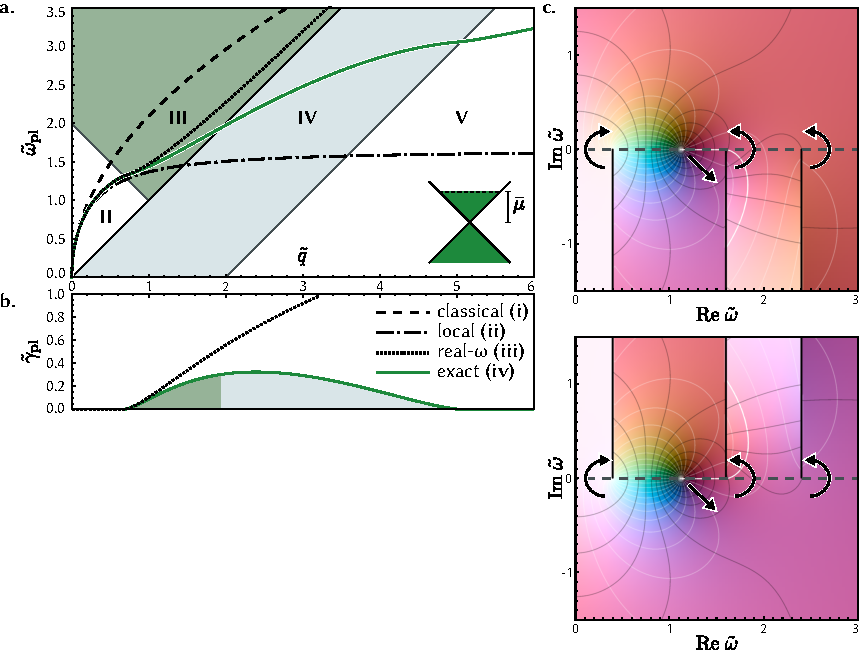
\includegraphics{figs/gr/PlasDisp.pdf}
 \caption[Complex frequency plasmon dispersion of equilibrium graphene]{
\label{fig:PlasDisp} \textbf{Complex frequency plasmon dispersion of
equilibrium graphene.}\small\\
\subA. Plasmon dispersion relation and \subB. loss of doped graphene in thermal
equilibrium.
Quantities are scaled to the chemical potential and Fermi velocity.
The exact \rpa solution \cfpd is plotted (green solid line) with the low-loss
approximation (black dotted line), the optical conductivity (black dot-dashed
line), and Drude model (black dashed line).
Regions of Landau damping are shown for interband (\III: green) and intraband
(\IV: gray) processes, as well as for quasi-loss-free regions (\II,\V: white).
Scaled coordinates are used where $\qtilAbs = \ħ\vF q/\μ$, $\ωtilpl =
\ħ\ωpl/\μ$
\subC. For a fixed $q$, the value of $\εRPA$ is plotted over a complex $\ωtil$
(\sec{f(z)}).
When the root crosses the real line, from the upper half-space to the lower,
branches must be rotated 180° such as not to pass over it.
Allowing the root to be found in a branch-free lower half-space.
}
\end{figure}

The \rpa plasmon dispersion can be solved for exactly.
Given the analytic form of the polarisability, \eq{analPolar}, the value of $\Π$
may be given directly as a function of a complex frequency.
The exact solution deviates from the low-loss approximation when the curve
enters the regime of Landau damping.
In Ref.~\cite{Pyatkovskiy2009} the exact solution is plotted up to the point
before the dispersion curve crosses the Fermi line.
In this work, this is extended to show the exact \cfpd solution
for any wavevector including in the intraband regime where $\vF q > \ω$
\cite{Page2015}.

The exact \cfpd is solved and shown in \figSub{PlasDisp}{.a} for plasmons of
zero-temperature equilibrium graphene with a finite chemical potential.
For comparison, this is shown alongside the low-loss approximation as
described in \eq{lowloss}, as well as solving for a \twod Drude conductivity and
a local ($q \→ 0$) optical conductivity approximation \cite{Falkovsky2007a}.
The curves are plotted on top of the regions in $(q,\ω)$ space where
single particle excitations are kinematically allowed (in green for interband,
and gray for intraband), i.e.
where the polarisability has finite imaginary part for real frequency and
wavevector.
The regions in white can not play part in absorption or emission processes, as
transitions here cannot fulfil conservation of momentum, and as such the
polarisability has zero imaginary part in these regions for real frequency and
wavevector.
For small wavevector, all solutions converge onto each other, before the Drude
model solution separates off.
Whilst in the quasi-loss-free region, the low-loss and \cfpd solutions are
identical, with the optical conductivity beginning to separate off.
Within the interband Landau damping regime, the low-loss and \cfpd solution
deviate, with the low-loss tracking alongside the Fermi line, being unable to
cross it.
The \cfpd however continues passing through the interband
Landau damping regime, over the Fermi line, through the intraband Landau damping
regime and out into the large wavevector quasi-loss-free regime.
Due to the singularity at $\ω = \vF q$, the low-loss approximation can never
cross the Fermi line, however the exact solution is able to bypass the
singularity having acquired a finite imaginary part, and enter into the intraband
absorption region.

In order to determine the roots of the dielectric function (\eq{εRPA}), one must
note that the polarisability function is multi-valued with branch cuts in the
complex-$\ω$ plane.
The form of the function as given in \eq{analPolar} is one configuration of the
branches of this multiply valued function, i.e. a configuration that gives
the correct value for real $q$ and $\ω$.
It is analytic in the upper-half plane with branch cuts along the real axis.
The branch-cuts themselves are not physical; different versions of the function
may be formulated which are identical in the vicinity of a particular value of
$\ω$ for which the branch cuts differ.
One can move smoothly from one branch to another in a process called
\emph{analytic continuation} where any path in a complex variable's space, i.e.
$\ω$ here, varies smoothly from one value to the next parameterised along the
path.
The analytic continuation along a path is unique as long as the path does not
pass through any singularities.

In order to solve for the dispersion relation, the wavevector $q$ is swept along
real values from zero, then for each value of $q$ the branches of the function
are chosen such that they are moved out of the way of the vicinity of the root in
$\ω$.
Practically this means for $\Im \ω > 0$, the branches, which hang from
branch-point singularities on the real axis that cannot be removed, are chosen
to point vertically and downwards (occupying the lower half space); and for
$\Im \ω < 0$, the branches point vertically and upwards.
When the branch configuration changes, there is the choice as to whether to
rotate each branch-cut clockwise or counter-clockwise,
chosen such that the branch cuts will never sweep over the root that is
being traced, as depicted in \figSub{PlasDisp}{.b}.

The resulting plasmon dispersion and loss curve that is retrieved from this
procedure (solid line in \fig{PlasDisp}) is continuous, with zero loss in the
regions of no Landau damping and smooth throughout the damping regions including
when crossing over the Fermi line.

\section{Nonequilibrium Polarisability} \label{sec:NEPol}
The polarisability is an important object in its own right, apart from its
inclusion in the plasmon dispersion and optical conductivity, it is used in
dynamic screening of the Coulomb potential
$\bar{V}_q = V_q / \εRPA(\q, \ω)$ \cite{Hill2009}.
The screening enters into higher-order processes such as carrier-carrier and
Auger processes \cite{Brida2013}
(Auger recombination, impact ionisation) as well as for
coupling to other bosonic fields such as scattering with optical phonons
\cite{Butscher2007,Rana2009,Wang2010}.
Calculating the polarisability in increasingly complicated electronic
configurations has been the subject of much research
\cite{Gonzalez1994,Wunsch2006,Vafek2006,Hwang2007,Ramezanali2009,Tomadin2013}.

\begin{figure}
 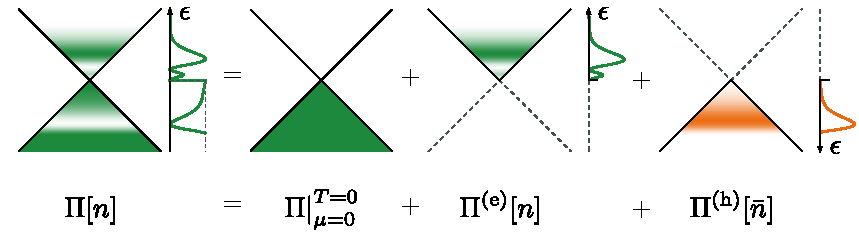
\includegraphics{figs/gr/NonEqDist.pdf}
 \caption[Nonequilibrium polarisability]{\label{fig:NonEqDist}
\textbf{Nonequilibrium polarisability.}\small\\
The nonequilibrium polarisability is a linear functional of the carrier
distribution $n(\έ)$ and can be decomposed into a background intrinsic
zero-temperature equilibrium polarisability plus contributions from
nonequilibrium electrons and holes.
}
\end{figure}

The Lindhard formula for graphene \eq{lindhard}, which was used to
derive the equilibrium polarisability, is noted to be a linear functional of the
carrier distribution $n(\έ)$.
Using only this and the fact that a zero-temperature Fermi distribution is
equivalent to a Heaviside Theta function,
$f(\έ - \μ, T=0) = \θ(\μ-\έ)$,
the graphene polarisability may be derived for any arbitrary nonequilibrium
carrier distribution.
Starting with the following linearity identity,
\begin{subequations}\subeq
\begin{align}
\Π[n] &=
\Π \left[ \int_{-\infty}^{\infty} \d\έ \:
\δ(\έ-\έ') n(\έ) \right]
\\ \nonumber
&= \int_{-\infty}^{\infty} \d\έ \:
\Π\left[ \δ(\έ-\έ') \right] n(\έ)
\\ \nonumber
&= \int_{-\infty}^{\infty} \d\έ \:
\Π\left[ \pd{f(\έ'-\έ, T=0)}{\έ} \right]
n(\έ)
\\
\Π[n] &= \int_{-\infty}^{\infty} \d\έ \:
\pd{\Π^{\T=0}_{\μ=\έ}}{\έ} n(\έ)
\;.
\end{align}
\end{subequations}
This form integrates over the sea of filled hole states, which is divergent as
it takes a limit of an ever growing Fermi-edge to negative infinity.
To regularise this integral one may separate off the carrier distribution into
an intrinsic part and contributions from electrons and holes,
as in \fig{NonEqDist}, i.e.
\begin{align}
n(\έ) =
\underbrace{ \θ(-\έ) }_\mathrm{intrinsic} +
\underbrace{ n(\έ) \θ(\έ) }_\mathrm{electrons} -
\underbrace{ \bar{n}(-\έ) \θ(-\έ) }_\mathrm{holes}
\;,
\end{align}
where $\bar{n}(\έ) = 1 - n(-\έ)$ is the hole distribution.
This leads to the following elegant form\footnote{
Assuming particle/hole symmetry, as usual, means
$\pd{\Π^{\T=0}_{\μ=-\έ}}{\έ} = \pd{\Π^{\T=0}_{\μ=\έ}}{\έ}$
and therefore,
$\Πe = \Πh$
}:
\begin{align}\label{eq:elegant}
\Π[n] &= \Π^{T=0}_{\μ=0} +
\int_0^\infty \d \έ \: \left[
  \pd{\Π^{T=0}_{\μ=\έ}}{\έ} n(\έ)
+ \pd{\Π^{T=0}_{\μ=-\έ}}{\έ} \bar{n}(\έ)
\right] \\
&= \Π^{T=0}_{\μ=0} + \Πe[n] = \Πh[\bar{n}]
\;.
\end{align}
The nonequilibrium polarisability is formed here of a background contribution
of a zero temperature intrinsic equilibrium added to terms for the particle and
hole plasmas.
This allows the calculation of any nonequilibrium polarisability for any
given carrier distribution $n(\έ)$ and is well suited to numerical evaluation,
more details of which will be given in \sec{hotCarriers}.
The formalism here is general, and particularly does not include any graphene or
approximation-specific features, such as band structure characteristics, relying
only on the linearity of the Lindhard formula, a feature of taking the leading
order term in \rpa, and in the absence of self-energy corrections.
This formalism is therefore applicable to calculating the polarisability and
dielectric function out of equilibrium of general \twod fermion gasses within
\rpa.

\subsection{Scale-free Representation} \label{sec:scale}
The conical band-structure of graphene, $\έ^s_\k = s \ħ \vF |\k|$,
does not define any energy scale,
which can be shown to lead to a universal behaviour, described by scale-free
coordinates.

Taking the Lindhard Formula, \eq{lindhard}, and scaling the dynamic variables,
$\q \rightarrow \q/a$, $\ω \rightarrow \ω/a$ and
carrier distribution, $n'(\έ) = n(a\έ)$, by a constant factor $a$, gives,
\begin{subequations}\subeq
\begin{align}
\Π[n](\q,\ω) &= \frac{g}{A} \sum_{s,s'=\pm} \sum_{\k}
M^{s s'}_{\k,\k+\q}
\frac{n(\έ^s_{\k}) - n(\έ^{s'}_{\k+\q})}
{\έ^s_{\k} - \έ^{s'}_{\k+\q} + \ħ\ω + \i\times0}
\\ \nonumber
&= \frac{g}{A} \sum_{s,s'=\pm} a^2 \sum_{\k/a}
M^{s s'}_{\frac{\k}{a},\frac{\k+\q}{a}}
\frac{n(a \έ^s_{\k/a}) - n(a \έ^{s'}_{(\k+\q)/a})}
{a \έ^s_{\k/a} - a \έ^{s'}_{(\k+\q)/a} + a\ħ\ω/a + \i\times0}
\\ \nonumber
&= a \frac{g}{A} \sum_{s,s'=\pm} \sum_{\k/a}
M^{s s'}_{\frac{\k}{a},\frac{\k+\q}{a}}
\frac{n'(\έ^s_{\k/a}) - n'(\έ^{s'}_{(\k+\q)/a})}
{\έ^s_{\k/a} - \έ^{s'}_{(\k+\q)/a} + \ħ\ω/a + \i\times0}
\\
\Π[n](\q,\ω) &= a \Π[n'] \left( \frac{\q}{a},\frac{\ω}{a} \right)
\;,
\end{align}
\end{subequations}
as a scaling rule.
Borrowing from the form of \eqSub{analPolar}{.a},
one can express polarisabilities in a form with all variables scaled to an energy
$\μbar$.
\begin{subequations}\subeq
\begin{align}
\Π[n(\έ)](\q,\ω) &= \frac{g\μbar}{8 \π \ħ^2 \vF^2}
\Πtil \left[ n(\έtil) \right]
\left( \frac{\ħ\vF\q}{\μbar},\frac{\ħ\ω}{\μbar} \right)
\\
&= \frac{g\μbar}{8 \π \ħ^2 \vF^2} \Πtil [ n ( \έtil ) ] (\qtil, \ωtil)
\;,
\end{align}
\end{subequations}
with the the following scaling definitions,
$\qtil = \ħ \vF \q / \μbar$,
$\ωtil = \ħ \ω / \μbar$, and
$\έtil = \έ / \μbar$,
where variables marked with a tilde are scaled to $\μbar$,
and the dimensionless $n(\έtil)$ replaces the absolute $n(\έ)$.

The universality becomes most clear when calculating the dielectric function,
\eq{εRPA} becomes,
\begin{align} \label{eq:εRPAdl}
\εRPA(\qtil,\ωtil) = 1 - \frac{\αg}{\qtilAbs} \Πtil(\qtil,\ωtil)
\;,
\end{align}
with the graphene fine-structure constant \cite{Jang2008,Hofmann2014},
\begin{align}
\αg = \frac{g}{4} \frac{\c}{\vF} \frac{\αf}{\εbar}
\;,
\end{align}
where $\αf \approx 1/137$ is the vacuum fine-structure constant.
Which for suspended graphene takes a value of $\αg \approx 2.2$.

Finally, it remains to cast the derivative form (\eq{elegant}) in dimensionless
terms.
\begin{subequations}\subeq
\begin{align}
\pd{\Π^{\T=0}_{\μ}}{\μ} &=
\pd{}{\μ} \Π[f(\έ-\μ, T=0)] (\q,\ω)
\\ \nonumber
&= \frac{g}{8 \π \ħ^2 \vF^2} \pd{}{\μtil} \left[ \έtil'
\Πtil_1 \left( \frac{\qtil}{\μtil}, \frac{\ωtil}{\μtil} \right) \right]
\\
& \coloneqq \frac{g}{8 \π \ħ^2 \vF^2} \Πtil'(\μtil; \qtil, \ωtil)
\;,
\end{align}
\end{subequations}
leading to the scale-free expression for polarisabilities of arbitrary carrier
distributions:
\begin{align}\label{eq:elegant2}
\Πtil[n](\qtil,\ωtil) = \Πtil_0 (\qtil, \ωtil) &+
\int_0^\infty \d \έtil \: \left[
  \Πtil'(\έtil; \qtil, \ωtil) n(\έtil)
+ \Πtil'(\έtil; \qtil, \ωtil) \bar{n}(\έtil)
\right]
\;,
\end{align}
with
$\Πtil_0 = \lim_{a \rightarrow 0}
a  \Πtil_1 \left( \qtil / a, \ωtil / a\right)$,
being the dimensionless form of the intrinsic polarisability.

Within the Dirac-cone approximation, specific form of these terms may
given as,
\begin{subequations}\subeq\label{eq:grPolKernel}
\begin{align}
\Πtil'(\έtil; \qtil, \ωtil) &=
-4 + 2 \frac{
\Gp \left( \frac{\ωtil + 2 \έtil}{\qtilAbs} \right) +
\Gp \left( \frac{\ωtil - 2 \έtil}{\qtilAbs} \right)
}{
\Gp \left( \frac{\ωtil}{\qtilAbs} \right)
}
\\
\Πtil_0 &= -\frac{\qtilAbs}{2} \frac{\π}{\Gp \left( \frac{\ωtil}{\qtilAbs}
\right) }
\;,
\end{align}
with,
\begin{align}
\Gp(z) &= \sqrt{1 - z^2}
\;,
\end{align}
\end{subequations}
for $\ωtil \rightarrow \ωtil + 0\i$.

As the solutions to \eq{εRPAdl} are independent of energy scale $\μbar$, all
dispersion curves of electronic configurations that are similar (equal but for
scale) can be mapped onto a single curve $\ωtil(\qtil)$ of dynamic variables
that are set to the same energy scale.

\section{Quasiequilibrium} \label{sec:quasieq}
The first nonequilibrium state of graphene to consider is the
quasiequilibrium where the electronic distribution in the conduction band and
the valence band can both be described by Fermi functions, with each having
their own separate chemical potential, albeit sharing a common temperature.
This serves as a first approximation to photoexcited graphene.
When graphene is externally pumped by photons, they may be absorbed creating
electron-hole pairs in a hot carrier distribution.
The hot carrier distribution then relaxes and each band thermalises
independently, assuming that intraband relaxation channels such as
carrier-carrier scattering are at least an order of magnitude faster (tens of
femtoseconds)
\cite{Dawlaty2008,Choi2009,Breusing2009,Breusing2011,Malic2011,Sun2012}
than interband recombination processes, which themselves can be ultrafast
\cite{George2008,Winnerl2011,Johannsen2013,Malard2013,Jensen2014}.
This leaves the system in a momentary state of population inversion
\cite{Kesler1987,Haug1989} from where stimulated emission processes may exceed
the rates of absorption allowing for net gain.
The quasiequilibrium is therefore a snapshot of an evolving system that is
modelled by a pair of Fermi distributions parameterised by electron and hole
chemical potentials, $\μe$, $\μh$ and temperature $\T$, which will seek to
return to equilibrium over time, as will be explored in \sec{npe}.

An alternative way to parameterise the system would be through the carrier
number and energy densities, $\Ne$, $\Nh$, $U$, which are found by summing over
wavevector states for each species, $s \in \{\mathrm{e}, \mathrm{h}\}$,
\begin{subequations}
\begin{align}
\Ns(\μs, \T) &= \frac{g}{A} \sum_\k f(\έ_\k^s - \μs, \T) \\
\Us(\μs, \T) &= \frac{g}{A} \sum_\k f(\έ_\k^s - \μs, \T)  \έ_\k
\;,
\end{align}
\end{subequations}
with the total energy density $U = \Ue + \Uh$.
These integrate to polylogarithm functions
\cite{Blundell2010},
\begin{subequations}
\begin{align}
\Ns(\μs, \Tc) &= -\frac{2}{\π}
\frac{(\kB \T)^2 \Li_2(-e^{\μs/\kB \T})}{(\ħ\vF)^2}
\\
\Us(\μ, \Tc) &= -\frac{4}{\π}
\frac{(\kB \T)^3 \Li_3(-e^{\μs/\kB \T})}{(\ħ\vF)^2}
\;.
\end{align}
\end{subequations}
The carrier number and energy density become useful when considering the
dynamics of the system, i.e. how it responds to external pumping such as
photoexcitation, and how it subsequently relaxes.

The result of \sec{NEPol} can be immediately applied to the case of a
zero-temperature quasiequilibrium.
Assuming electrons and holes can be described respectively with chemical
potentials $\μe$, $\μh$, then their distribution becomes,
\begin{subequations}\subeq
\begin{align}
     n  = \f(\έ-\μe,T = 0) = \θ(\μe-\έ) \\
\bar{n} = \f(\έ-\μh,T = 0) = \θ(\μh-\έ)
\;.
\end{align}
\end{subequations}
Inserting into \eq{elegant2} yields,
\begin{align}
\Πtil_{\μe,\μh}(\qtil,\ωtil) &= \Πtil_0 (\qtil, \ωtil) +
\int_{0}^\infty \d \έtil \: \Πtil'(\έtil; \qtil, \ωtil)
\left[
 \θ(\μe-\έ) + \θ(\μh-\έ)
\right]
\;.
\end{align}
Then by extension of the integration range of \eq{elegant2} leads to,
\begin{subequations}\subeq
\begin{align}
&\Πtil_{\μe,\μh}(\qtil,\ωtil) = \Πtil_0 (\qtil, \ωtil) \\ \nonumber &+
\int\limits_{-\infty}^\infty \d \έtil \: \Πtil'(\έtil; \qtil, \ωtil)
\left[
 \θ(\μe-\έ) - \θ(-\έ) + \θ(\μh-\έ) - \θ(-\έ)
\right]
\\ \label{eq:quasieqμ}
&= \frac{\μe}{\μbar} 
\Πtil_1 \left( \frac{\qtilAbs \μbar}{\μe} , \frac{\ωtil \μbar}{\μe} \right) +
\frac{\μh}{\μbar} 
\Πtil_1 \left( \frac{\qtilAbs \μbar}{\μh} , \frac{\ωtil \μbar}{\μh} \right) -
\Πtil_0 (\qtilAbs, \ωtil)
\;.
\end{align}
\end{subequations}

\begin{figure}
 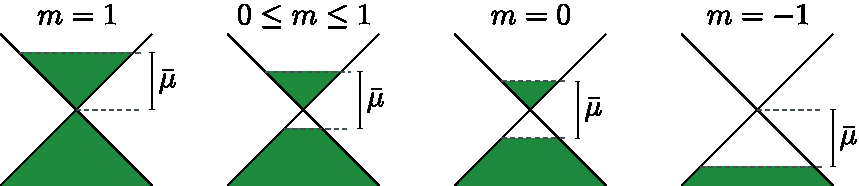
\includegraphics{figs/gr/MDist.pdf}
 \caption[Carrier imbalance parameter]{ \label{fig:MDist}
\textbf{Carrier imbalance parameter.}\small\\
The parameter $m$ labels graphene variously
in a state of n-doped equilibrium ($m = 1$),
n-doped photoinverted quasiequilibrium ($0 \le m \le 1$),
intrinsic photoinverted quasiequilibrium ($m = 0$),
and p-doped quasiequilibrium ($m>0$).
}
\end{figure}

It makes sense to chose $\μbar = \μe + \μh$ as the scale parameter in this case,
which allows us to further define the free parameter - the carrier imbalance
parameter,
\begin{equation}
m = \frac{\μe - \μh}{\μe + \μh}
\;.
\end{equation}
This describes the imbalance of the electrons and
holes in the carrier density, and ranges from $m=-1$ where $\μe = 0, \μh =
\μbar$; to $m = 0$ where $\μe = \nicefrac{\μbar}{2}, \μh = \nicefrac{\μbar}{2}$;
to $m = +1$ where $\μe = \μbar, \μh = 0$.
This is illustrated in \fig{MDist}.
Here only the range $m \in [0, 1]$ will be considered, as negative values of $m$
return equivalent physics to positive ones due to the symmetry of the
conduction and valence bands in the Dirac cone approximation.
With this, \eq{quasieqμ} becomes,
\begin{equation}
\Πtil_{m}(\qtil,\ωtil)
= \frac{1+m}{2} 
\Πtil_1 \left( \frac{2 \qtilAbs}{1+m} , \frac{2 \ωtil}{1+m} \right) +
\frac{1-m}{2} 
\Πtil_1 \left( \frac{2 \qtilAbs}{1-m} , \frac{2 \ωtil}{1-m} \right) -
\Πtil_0 (\qtilAbs, \ωtil)
\;.
\end{equation}

When there are carriers in the conduction band above a range of vacant states
in the valence band, there is a \emph{population inversion}.
In this state, electrons and holes can spontaneously recombine emitting a
plasmon, but they can also recombine, emitting a coherent plasmon through
stimulation by free plasmons on the sheet.
Electrons in the conduction band, below $\μe$, may recombine with
holes in the valence band below $\μh$.
As such plasmons with energies below $\ħ\ω < \μe + \μh = \μbar$ may experience
gain.
The more similar the level of electron and hole populations are, the more phase
space will be available for stimulated emission processes, from the
maximal case of a symmetric (intrinsic) inversion for $m=0$ down to no phase
space for $m = \pm 1$ where there is no population inversion.
Plasmons outside this frequency range may be absorbed, as was the case for
equilibrium graphene, along with plasmons which can induce intraband
transitions.

\subsection{Intrinsic Graphene}

\begin{figure}
 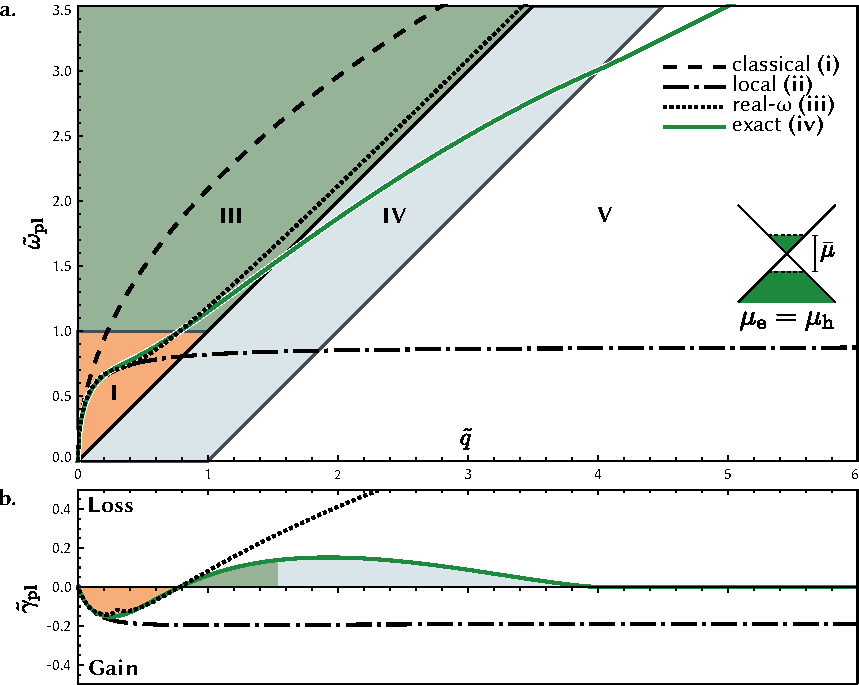
\includegraphics{figs/gr/PlasDispInv.pdf}
 \caption[
Complex frequency plasmon dispersion of photoinverted graphene]{
\label{fig:PlasDispInv} \textbf{Complex frequency plasmon dispersion of
photoinverted graphene.}\small\\
\subA. Plasmon dispersion relation and \subB. loss of intrinsic graphene in
photoinverted quasiequilibrium.
The exact \rpa solution \cfpd is plotted (green solid) with the low-loss
approximation (black dotted), the optical conductivity (black dot-dashed), and
Drude model (black bashed).
Regions of recombination are shown (\I: orange) and regions for interband
(\III: green) and intraband (\IV: gray) damping, as well as for
quasi-loss-free regions (\V: white).
}
\end{figure}

The case of intrinsic inversion should be given some special attention.
Optical excitation creates electrons and holes in a pairwise manner,
given the equivalence of the conduction and valance band.
Considering an intrinsic sheet of graphene that is optically pumped,
the resulting quasiequilibrium after the initial excitation will have equal
chemical potentials $\μe = \μh$, i.e. the imbalance parameter $m = 0$.
The polarisability in this case takes the simplified form,
\begin{equation}
\Πtil_{m=0}(\qtil,\ωtil)
= 2 \Πtil_1 ( \qtilAbs, \ωtil) -
\Πtil_0 (\qtilAbs, \ωtil)
\;.
\end{equation}
The \cfpd can be solved for this photoinverted case and the result is plotted
in \fig{PlasDispInv} in analogy to \fig{PlasDisp}, with the equivalent
approximative solutions also plotted.
Qualitatively, the curve is similar, following the Drude model curve for small
$\qtilAbs$.
However, for frequencies $\ωtilpl < 1$, the plasmons are susceptible
to stimulated emission of plasmons due to recombination of electron/hole pairs.
This gives a negative decay rate $\γtilpl$ which characterises amplification
i.e. plasmon gain.
This gain falls to zero for $\ωtilpl = 1$ where there are no inverted electron
hole pairs that have such an energy difference.
For frequencies above this,
the plasmon enters the interband Landau damping regime and has a positive decay
rate again.
At $T=0$ the regions where emission and absorption processes occur are sharply
separated at $\ωtilpl = 1$: not only is the net rate zero here, but the rates
for the separate absorption and emission processes go to zero, with emission
having zero rate above $\ωtilpl = 1$ and absorption having zero rate below.
For finite temperature, the two rates will smear into all frequencies as
the Fermi-edge is smeared, as will be discussed in \sec{lowT}.
The curve then continues through the interband and intraband regions in a manner
similar to the equilibrium plasmon.

In contrast to the \cfpd, the low-loss approximation curve displays a
distinctive and spurious dip in the gain region that arises from
performing a Taylor expansion too close to a branch singularity at
$\ωtil=1-\qtilAbs$.
This curve, in common with its equilibrium counterpart, cannot cross the Fermi
line, but rather asymptotically approaches it with a loss that continues
growing.

The dispersion under the local optical conductivity model limits to a
finite value.
Given that its model is local and can only see vertical
transitions i.e. $q\→0$, the loss is negative over the entire curve and as such
only interband recombination processes are accounted for.

In this section, it has been shown how the inverted plasmon dispersion differs
from that of equilibrium, how the \cfpd solution of a nonlocal \rpa
polarisability is able to return accurate results in all absorption/emission
regimes that other approximations can not.
The \cfpd also yields the exact plasmon gain/loss rate within the \rpa, allowing
for further analysis.

\begin{figure}
 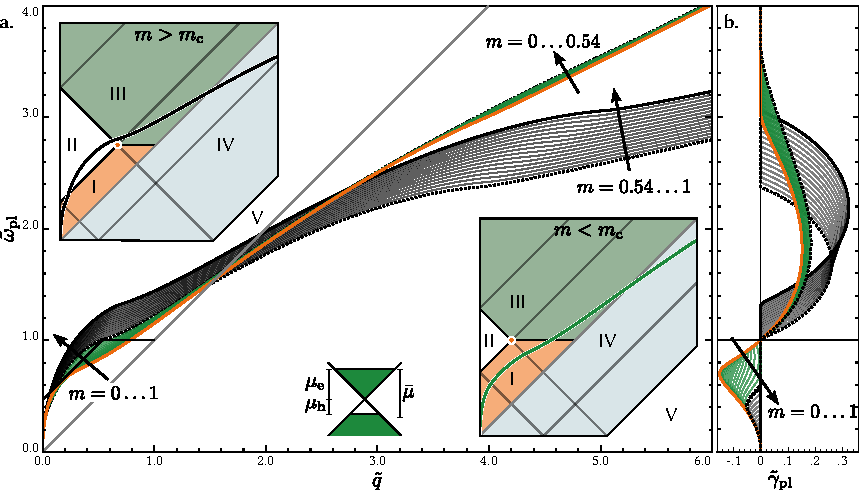
\includegraphics{figs/gr/Mparam.pdf}
 \caption[Complex frequency plasmon dispersion for varying carrier imbalance]{
 \label{fig:Mparam}
 \textbf{Complex frequency plasmon dispersion for varying carrier imbalance}
 \small\\
\subA. Complex frequency dispersion curves of extrinsic photoinverted graphene
for a varying carrier inversion parameter, $0 < m < 1$.
The curves split into two bundles at a critical value $\mc$.
Insets show representative curves either side of the splitting, shown against
regions of Landau damping and recombination, the black curves passing above the
critical branch point (orange dot) and the green curves below.
\subB. Loss plotted over the frequency.
For frequencies less than $1$, the curves smoothly morph into each other,
whereas past this range, a distinct splitting occurs.
}
\end{figure}

\subsection{Extrinsic Graphene}
The chemical potential of Graphene can be set by an external gate voltage, or by
chemical doping of the sample, or indeed by interaction with the substrate.
This has the effect of adding an excess of one species of carrier, either
electrons or holes.
When there is a difference between the number of electrons and
holes, i.e. $\Ne \neq \Nh$, the carrier imbalance parameter, $m$, of extrinsic
graphene will take an intermediate value between 0 and 1.

\Fig{Mparam} shows the regions in reciprocal space for which plasmons
experience gain (\I: orange), interband absorption (\III: green), intraband
absorption (\IV: gray), and regions with no phase space for these processes
(\II: white).
The relative sizes of these regions change with $m$, starting from equilibrium
at $m=1$ where the gain region (\I) is vanishing and there is a large
triangular loss-free region (\II), down to $m=0$ at full inversion where the
loss-free triangle has shrunk to vanish, leaving a gain triangle in place.
These extremal cases can be seen in \figs{PlasDisp}{PlasDispInv}.
For intermediate values the gain region becomes a trapezium with its upper
vertex defining its size, located at $(\qtilAbs = m, \ωtil = 1)$.
The loss free region remains a triangle as $m$ is varied.

A range of \cfpd curves for values of $m$ between 0 and 1 are plotted.
The extremal values of $m=1$ (doped equilibrium), and $m=0$ (intrinsic
inverted) are drawn with the swarm of intermediate curves in-between.
Two different families of curves are to be found, one set that passes from
interband gain to interband loss directly, and the other that passes through
the quasi loss-free region in-between.
The first set includes the $m=0$ curve, and each of the curves in the bundle
follow the character of this curve tightly.
The latter bundle includes the $m=1$ curve, and although all the curves smoothly
vary from one to another, there is more variance in this bundle.
Whereas these bundles start out together, they start to diverge for
$\ωtil > 1$, and varying $m$.
This splitting is more clearly seen when considering the loss.
The values of $\ωpl$ are monotonic in $q$, which allows the loss $\γpl$ to be
plotted, in a more instructive manner as a function of frequency instead of
wavevector.
This separates the gain spectrum into a gainy part, for $\ωpl < 1$, and a lossy
part for $\ωpl > 1$.
The loss shows a step change between the bundles about this point.
The curves for a low-$m$ pass through $(\ωpl=1, \γpl=0)$ with finite gradient,
whereas the low-m curves are already trailing with a zero imaginary part having
entered the quasi-loss-free regime beforehand.
As the dispersion bundles have separated, the frequencies at which the curves
leave the intraband absorption region, and hence when the loss returns to zero,
do not match between each bundle.
Even though the curves themselves are smooth and within a bundle, they show a
marked bifurcation between the bundles.
The mathematical origin of this is the curves entering onto a different leaf of
the dielectric function's Riemann sheet.
A more robust physical explanation is more elusive, and will remain the subject
for future investigation.
The critical value of $m$ for which the transition occurs can be solved for.
Since the character of the dispersion curve is dependent on which side of the
critical branch point (orange point) it passes.
The branch point is located at $(\qtilAbs = m,\ωtil=1)$, where regions \I, \II
and \III come together, so finding the critical branching value is finding the
curve that passes through that point, i.e.
\begin{equation}
1 - \frac{\αg}{\mc}\Πtil_{m=\mc}(\mc,1) = 0
\;.
\end{equation}
For the case of suspended graphene, this takes a value of
$\mc \approx 0.538$.

In this section, the idealised case of graphene in zero-temperature
quasiequilibrium, which approximates the state of photoexcited graphene tens of
femtoseconds after the initial excitation, was studied.
The loss/gain profile was extracted for all curves parameterised by the carrier
imbalance parameter, $m$, and scaled to the energy $\μbar = \μe + \μh$.
A discontinuous behaviour was observed which separates the curves into a family
of intrinsic-like curves and extrinsic-like ones.

%As the polarizability appears in the Helmholtz free energy 
%\cite{Vafek2007,Ramezanali2009,Faridi2012}

\section{Collision Loss and Temperature} \label{sec:coltemp}
This section improves on the polarisability model by considering
collision losses, and then the impact of finite
temperature on the \cfpd and gain spectra of photoinverted graphene.

\subsection{Collision Loss}

\begin{figure}
 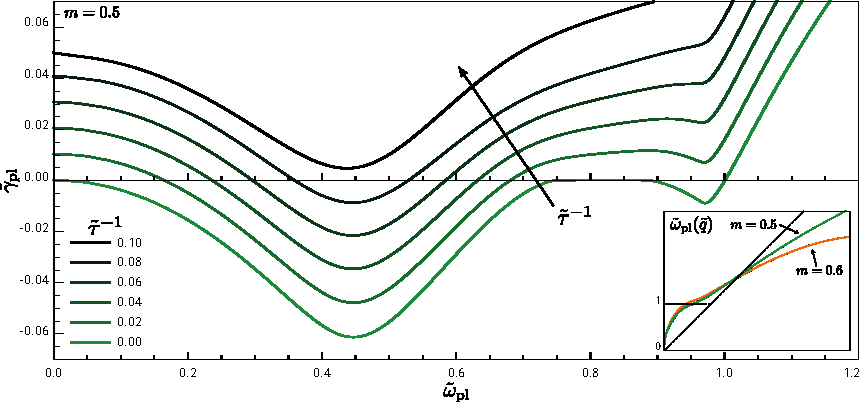
\includegraphics{figs/gr/Col.pdf}
 \caption[Impact of collision loss on plasmon decay rate]{ \label{fig:Col}
\textbf{Impact of collision loss on plasmon decay rate.}\small\\
Decay rate, at $m=0.5$, as collision loss is added with with scaled rates
$\τtil^{-1}$ from $0$ to $0.1$.
The corresponding plasmon dispersion is plotted inset for curves before and
after the critical splitting (green and orange lines respectively) to no
significant variation with collision rate.
}
\end{figure}
Thus far graphene has been portrayed with its only source of loss coming from
Landau damping.
This so-far overlooks Drude losses, the presence of which is universal in
traditional metal plasmonics \cite{Tassin2012}.
In the simplest model, effects such as electron collisions with impurities,
phonons \cite{Yan2013}, and other electrons, can be characterised by a
collective collision time $\τ$ in the femtosecond range \cite{Jablan2009}.
Such effects vary from sample to sample \cite{Dawlaty2008,Dawlaty2008a} and
through interaction with a substrate \cite{Scharf2013}.
In a first model, $\τ$ is kept as a free parameter.
The effect of collision loss on a polarisability function is properly treated by
making the transformation \cite{Mermin1970}:
\begin{equation} \label{eq:Mermin}
\Πtil_{\τtil}(\qtil, \ωtil) = \frac{(\ωtil + i \τtil^{-1})
 \Πtil(\qtil, \ωtil + i \τtil^{-1})}
{\ωtil + i \τtil^{-1}  \Πtil(\qtil,\ωtil + i \τtil^{-1}) / \Πtil(\qtil,0)}
\;,
\end{equation}
which conserves local particle number, in contrast to the more simplistic
addition of a uniform imaginary part,
$\ωpl - i \γpl \→ \ωpl - i \γpl - i \τ^{-1}$,
which does not.
\Eq{Mermin} can be applied to any of the polarisabilities introduced so far to
solve for the \cfpd in cases of photoinversion.
\Fig{Col} shows the effect on the loss spectrum of adding finite collision
loss in the range,
$\τtil^{-1} \in [0, 0.1]$ where $\τtil^{-1} = \ħ \τ^{-1}/\μbar$.

The first thing of note is that the dispersion is not significantly affected by
the incorporation of collision loss, and neither is the critical carrier
inversion parameter $\mc$ which separates the two bundles.
Dispersion curves are plotted for two values of $m$ and various values of
$\τtil$, which sit almost exactly on top of each other.
What does change is the loss spectrum, which shifts by around $\τtil^{-1} / 2$.
The curve also flattens out with the minimum becoming shallower for increasing
$\τtil^{-1}$.
For a scale parameter of $\μbar = 0.2\eV$, the maximum value of
$\τtil^{-1} = 0.1$ corresponds to a collision time of $\τ = 16\fs$.
At this collision rate all of the gain is extinguished, however for rates below
this, there are frequency bands for which the collision loss is compensated by
recombination, and the plasmons can be undamped and even still
amplified.

\subsection{Low Temperatures} \label{sec:lowT}
The approximation that photoinverted graphene will relax to a quasiequilibrium
can be improved by generalising the polarisability to finite temperatures.
This question has been first addressed in the literature for finite temperature
equilibria \cite{Ramezanali2009} but the form does not allow for the insertion
of complex variables, nor hence the calculation of the \cfpd.

\begin{figure}
 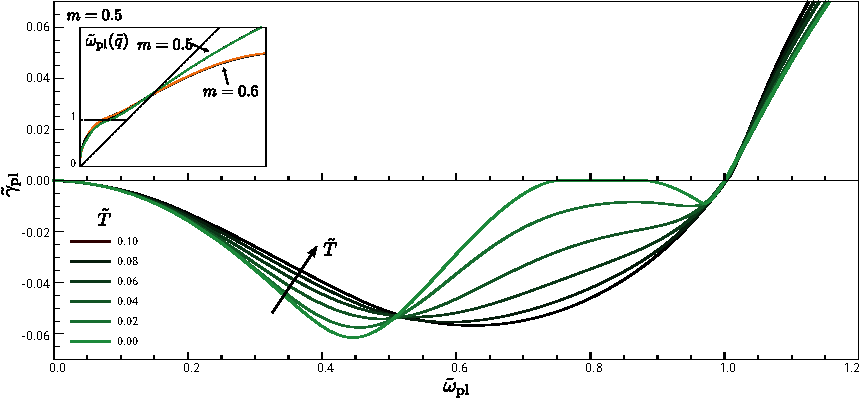
\includegraphics{figs/gr/LowTemp.pdf}
 \caption[Impact of temperature on plasmon decay rate]{ \label{fig:LowTemp}
\textbf{Impact of temperature on plasmon decay rate.}\small\\
Decay rate, at $m=0.5$, for scaled temperatures $\Ttil$ from $0$ to $0.1$.
The corresponding plasmon dispersion is plotted inset for curves before and
after the critical splitting (green and orange lines respectively) to no
significant variation with temperature.
}
\end{figure}

The electronic distribution of a finite temperature quasiequilibrium can be
represented as a correction to the zero temperature step function about the
Fermi-level as illustrated in \fig{LowTemp}.
Due to the linearity in the electron distribution of the polarisability, an
expression similar to \eq{elegant2} can be derived,
\begin{align}
\Πtil^{\Ttil}_m &= \Πtil_m +
\int_0^\infty \d \έtil \:
 \Πtil'(\έtil)
  \big(
   \δ f(\έtil-\μetil,\Ttil) + \δ f(\έtil - \μhtil, \Ttil)
  \big)
\;,
\end{align}
with $\δ f(\έtil-\μtil,\Ttil) = f(\έtil-\μtil,\Ttil) - f(\έtil-\μtil,0)$,
or breaking this down into separate integral components,
\begin{align} \label{eq:lowTpol}
% As a side note, I wonder how many Star-Trek characters I can turn into
% variable names.
\Πtil^{\Ttil}_m = \Πtil_m
&+\int_{\μetil}^\infty \d \έtil \:
  \Πtil'(\έtil) 
  \f(\έtil-\μetil,\Ttil)
 -\int_0^{\μetil} \d \έ \:
  \Πtil'(\έtil) 
 \f(\μetil-\έtil,\Ttil)
\\ \nonumber
&+\int_{\μhtil}^\infty \d \έtil \:
  \Πtil'(\έtil) 
  \f(\έtil-\μhtil,\Ttil)
 -\int_0^{\μhtil} \d \έ \:
  \Πtil'(\έtil) 
 \f(\μhtil-\έtil,\Ttil) 
\;.
\end{align}
This expression gives the finite temperature polarisability as a zero
temperature component plus finite temperature corrections.
This can now be used to calculate finite temperature \cfpd curves, however a
subtlety needs to be addressed.
The kernel of the integral, $\Πtil'(\έtil;\qtil,\ωtil)$ has branch points in
$\ωtil$ space which vary in position with $\έtil$, which is integrated over.
It is weighed by Fermi functions that peak closest to the respective chemical
potentials and decay exponentially away from this.
It is therefore a good approximation, whilst $\Ttil$ is small, to fix the branch
points at $\έtil$ to the \emph{centre of mass} of the weight functions.
The technical details of branch specification are detailed in \sec{branchcuts}.

The gain/loss spectrum $\γpl(\ωpl)$ is plotted (in analogy to \fig{Col}, in
\fig{LowTemp}) for values of $\Ttil$ varying between $0$ and $0.1$ for an
inversion of $m=0.5$.
These parameters correspond to a range of temperatures
$T \in [0,232.1]\K$ for a scale of $\μbar = 0.2\eV$.
As temperature increases, the gain peak blueshifts and broadens with the bimodal
nature at $\Ttil=0$ becoming a single peak.
The peak gain value does not significantly diminish in this temperature range.
Again, the dispersion curves $\ωpl(\qtilAbs)$, are not significantly affected on
either side of the bundle splitting, though the critical parameter shifts
slightly from $\mc \approx 0.56$ for $\Ttil = 0.1$ to $\mc \approx 0.538$ at
zero temperature.

A point of note here is that the transition between gain and loss remains at
$\ωtil = 1$ for all temperatures.
At zero temperature, this would be the frequency above which the phase
space of emission processes vanishes and that of absorption processes begins.
For finite temperature, the smearing of the Fermi functions ensures that there
is phase space for emission and absorption processes both above and below
$\ωtil = 1$, however the net rate is balanced exactly at this point.

\begin{figure}
 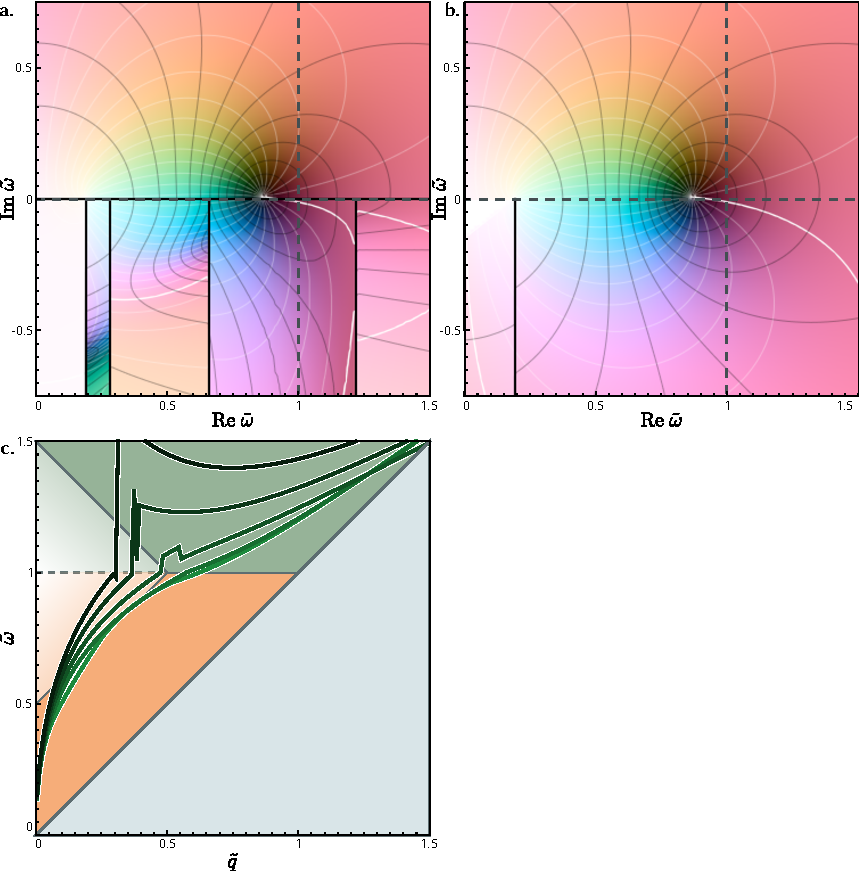
\includegraphics{figs/gr/AnalyticTemp.pdf}
 \caption[Limitation of low-temperature polarisability approach]
 {\label{fig:AnalyticTemp}
 \textbf{Limitation of low-temperature polarisability approach.}\small\\
 The solution space of $\εRPA(\qtilAbs,\ωtil)$ over a complex $\ωtil$ is
 plotted in \subA. and \subB. for quasiequilibrium graphene with $\Ttil=0.5$,
 $m=0.5$ at $\qtilAbs = 0.2$.
 The root is the encircled black spot, as described in \sec{f(z)}.
 \subA. uses the method of \sec{lowT}, and is analytic in the upper half-plane,
 but not in the lower, this can be seen as the contour lines do not intersect at
 right angles.
 \subB. uses the method introduced in \sec{hotCarriers}, and is analytic
 everywhere (apart from branch points).
 \subC. shows dispersion curves for temperatures varying from $\Ttil \in
 [0,0.5]$, they are correct for $\ωtilpl < 1$ while the complex solution is in
 the upper half-plane, but breaks down for $\ωtilpl > 1$.
}
\end{figure}

The approximation of treating the branches of \eq{lowTpol} at single points
begins to break down for $\Ttil \gtrsim 0.2$, see \fig{AnalyticTemp}.
This is because although \eq{lowTpol} is analytic in the top-half $\ωtil$ plane,
it is not so in the bottom half, such that when the plasmon transitions from
gain to loss (i.e. at $\γpl = 0, \ωpl = 1$), the values of the polarisability
are no longer strictly valid.
It should be clarified however that the dispersion curves and loss spectrum for
$\qtilAbs$ before $\ωpl(\qtilAbs) < 1$ are valid and are exact \cfpd solutions.
A more rigorous treatment of the nonequilibrium polarisability is required,
which will be treated in the next section.

\section{Hot Carriers} \label{sec:hotCarriers}
In order to calculate the \cfpd for arbitrary carrier distributions, one needs
to evaluate the integral of \eq{elegant} and interpret this as a complex
contour integral in $\έtil$.
Only one of the integral terms is considered here,
\begin{align}\label{eq:neqKernel}
\Π[n](\qtil,\ωtil) = \int_0^\infty \d \έtil \: \Πtil'(\έtil; \qtil, \ωtil) 
n(\έtil) + \ldots
\end{align}
This presents itself as an integral along the real axis from $\έtil = 0$ to
$\έtil = \infty$, though any path through the complex $\έtil$ plane with the
same endpoints will yield the same value so long as the the new path can be
deformed onto the original in a continuous manner, without crossing any of the
integrand's singularities.

There are two sources of singularities: from the kernel,
$\Πtil'(\έtil; \qtil, \ωtil)$, and from the distribution,
$n(\έtil)$.
The particular character of each is dependent on details of their functional
form.
Singularities in the kernel may move around in $\έtil$ space with changes in the
dynamic variables $\qtil$ and $\ωtil$, whereas the singularities in the
distribution are fixed.
To perform analytic continuation on $\Π[n](\qtil,\ωtil)$ over a complex $\ωtil$
is equivalent to evaluating the integral \eq{neqKernel} over a path that doesn't
cross any of the singularities as $\ωtil$ varies.

For the form of $\Πtil'(\έtil)$ as given in \seqs{grPolKernel},
there are four square-root branch point singularities located at,
\begin{equation}\label{eq:kernelSings}
\έtil^s_t = \pm_t  \frac{\ωtil \pm_s \qtilAbs}{2}
\;,
\end{equation}
with $s,t \in \{ + , - \}$, and four leaves of the function, two from each of
the square root terms in the numerator.
The leaf of the function for the start point of the contour is set such that
$\Πtil'(\έtil=0) = 0$, this choice ensures that the polarisability reduces to
its equilibrium form ($\Πtil_1$, see \eq{analPolar}) for a zero-temperature
Fermi distribution, $n(\έtil) = \θ(\έtil - 1)$.

To solve for the dispersion relation, the wavevector $\qtilAbs$ is scanned over
real values starting from $\qtilAbs = 0$.
Each possible $\ωtil(\qtilAbs)$ puts the branch points $\έtil^s_t$ in a
different position.

\subsection{Fermi Distribution}
The first nonequilibrium plasmon dispersion to solve for is the finite
temperature intrinsic quasiequilibrium, i.e. $n(\έtil) = \bar{n}(\έtil) =
\f(\έtil - \μtil, \Ttil)$, a Fermi distribution of electrons and holes in the
conduction and valence bands respectively, with matching chemical potentials.

The carrier distribution carries its own set of singularities, fixed in
position in $\έtil$ space.
Fermi distributions have poles at the Matsubara frequencies
\begin{equation}
\έtilM_n = \μtil + \i (2n + 1) \π \Ttil
\;.
\end{equation}

\begin{figure}
 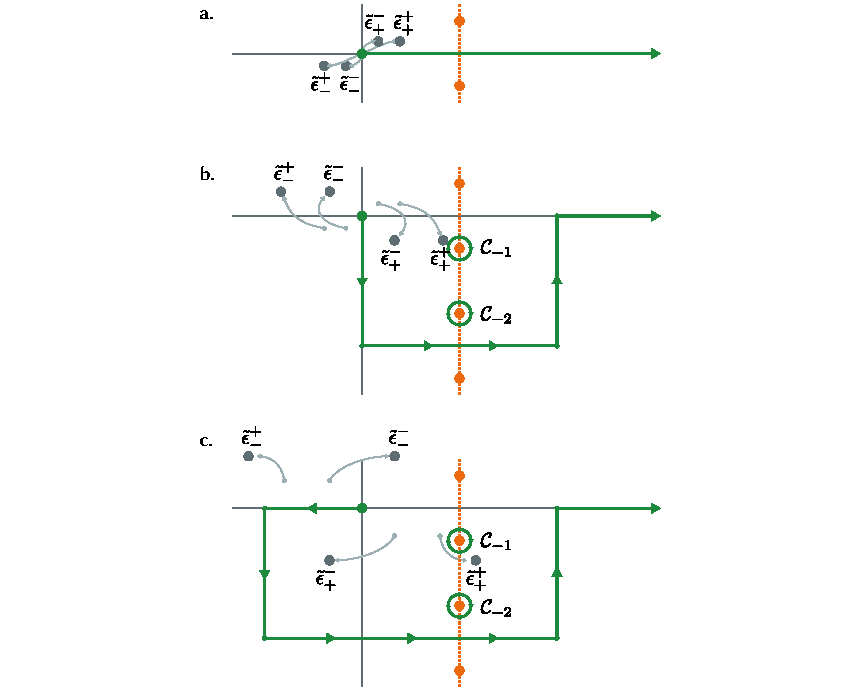
\includegraphics{figs/gr/Contour.pdf}
 \caption[Polarisability as a complex contour integration]{\label{fig:Contour}
 \textbf{Polarisability as a complex contour integration.}\small\\
The polarisability is calculated as a contour (green) in complex $\έtil$ space.
There are two types of singularity, branch points (grey), which move with
$(\qtilAbs,\ωtil)$ and poles (orange) which are fixed in place.
\subA. is the contour for small values of $\qtilAbs$, evaluated over
$[0,\infty)$.
The contour is deformed in \subB. to include a number of the Matsubara poles
such that the branch points can move within the lower half-space.
In \subC. the contour is further deformed to allow the $\έtil^-_+$ to move into
the bottom-left quadrant.
}
\end{figure}

The deformation of the integration contour can be generalised to be able to pass
over simple poles, so long as for each pole the contour crosses, the
contribution of that pole ($2 \π \i$ times the residue about the pole) is
subtracted from the final result.
For a Fermi distribution, the integral around an infinitesimal closed loop about
each pole has the form,
\begin{equation}
\oint_\Cn \! \d\έtil \: \f(\έtil - \μtil, \Ttil) \Πtil'(\έtil) =
% 2 \π \i \res(\Πtil',\έtilM_n) =
- 2 \π \i \Ttil  \Πtil'(\έtilM_n)
\;,
\end{equation}
which is equal to the value of the contour integral step-changes by as
each pole is taken through the contour.

The movement of the singularities of the kernel along solutions to the
dispersion relation, $\έtil^s_t(\qtilAbs,\ωtilpl(\qtilAbs))$, can be
accounted for.
Their imaginary part is given by $\Im \ωtil / 2$ (\eq{kernelSings}), which will
be positive for plasmons with gain, and negative for loss.
As in the zero temperature case, and low temperature solutions (\sec{lowT}), the
imaginary part starts positive, for a gain region before entering the lower
half-space for the Landau damping regime.
In order to allow the branch singularities to enter the lower $\έtil$
half-space, the original horizontal line contour (\figSub{Contour}{.a}) can be
deformed, by passing over any number of the Matsubara poles in the lower half
space to give a clear area for the branch points to pass through
(\figSub{Contour}{.b}).
Then for higher values of $\qtilAbs$, the dispersion will enter the intraband
regime and the branch points $\έtil^-_\pm$ will cross the imaginary axis.
This space can also be opened out, once $\ωtil$ has crossed the real axis, and
requires no further poles to be encircled (\figSub{Contour}{.c}).

\begin{figure}
 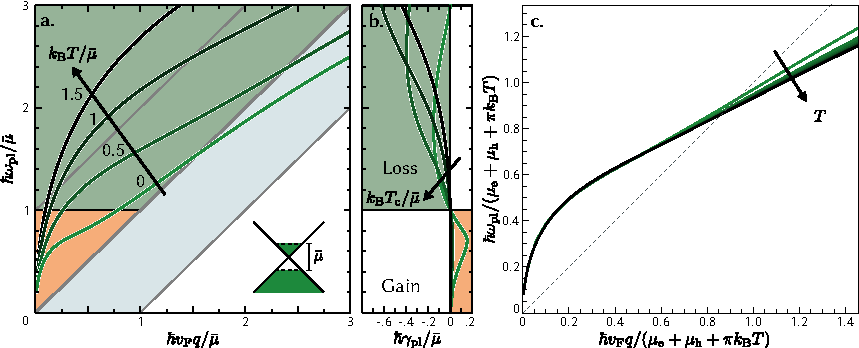
\includegraphics{figs/gr/TempScan.pdf}
 \caption[High temperature plasmon dispersion curves]{\label{fig:TempScan}
\textbf{High temperature plasmon dispersion curves.}\small\\
\subA. Dispersion and \subB. loss curves of intrinsic photoinverted
graphene, for temperatures varying $\Ttil \in [0, 1.5]$.
\subC. Curves are rescaled by a factor $1 + \π \Ttil$, they limit to
a universal behaviour for increasing $\Ttil$, this is at the expense of not
being able to draw regions of Landau damping and recombination.
% add more curves (up to Τ = 4 step 0.5),
% increase range (q to 6 ω to 4)
}
\end{figure}

Following this procedure, \eq{εRPAdl} can be solved for to find the plasmon
dispersion curves for varying temperature. \Fig{TempScan} plots these for
suspended graphene with symmetric carrier distributions.
As $\Ttil$ increases, each successive curve becomes steeper.
The increased steepness means that the dispersion curves stay in the gain
region for shorter intervals of $\qtilAbs$, whilst remaining in the Landau
damping regime ($\ωtil \gtrsim \qtilAbs - 1$) for longer.
This manifests itself as a blueshift in the absorption peak and with the peak
value of absorption increasing.
Despite this, the absorption curves come out shallower for frequencies
immediately above $\ωtil = 1$, as the phase-space for gain processes bleeds into
this regime.

If the curves are rescaled such that $\μbar = \μe + \μh + \π \kB T$ rather than
the usual $\μbar = \μe + \μh$, then the curves begin to align on top of each
other.
This allows high temperature curves to be estimated without calculation from
lower temperature ones.

\subsection{Non-Fermi Distribution}
Having shown the complex contour method applied to calculating the
polarisability of high-temperature quasiequilibrium Fermi distributions,
we turn to the question of calculating for arbitrary (isotropic) nonequilibrium
carrier distributions.
A case that one may wish to consider is that of a graphene sheet optically
pumped by an external field.
Here carriers are excited vertically from the valence to the conduction band,
generating electron hole pairs in a distribution with energies centred on
$\έ = \pm\ħ\ωpump/2$ and with a width of $\ħ\γpump$ \cite{Song2015}.

A model for this distribution would be a Gaussian function,
$g(z) = e^{-z^2/2}$, 
added to a finite temperature Fermi function background, i.e.
\begin{equation} \label{eq:simpleHot}
  n(\έ)
= n_0 g \left( \frac{\έ -\ħ\ωpump/2}{\γpump} \right)
+ f(\έ - \μs,\T)
\;,
\end{equation}
where $n_0$ is the carrier occupation number at the top of the photoinversion
peak, which will be a function of the pump beam intensity and duration.


\begin{figure}
 \includegraphics{figs/gr/GaussPade.pdf}
 \caption[Padé approximant for a Gaussian]{ \label{fig:GaussPade}
\textbf{Padé approximant for a Gaussian.}\small\\
\subA. Complex plot (\sec{f(z)}) of a Gaussian.
\subB. Its $(4,8)$ Padé approximant, showing 4 roots and 8 poles.
\subC. The two are compared as functions of a real variable for the Gaussian
(green), and its approximant (orange) showing additional side lobes.
}
\end{figure}
The Gaussian function is well behaved in the sense that it has no singularities
in the complex plane, however it diverges super-exponentially along the
imaginary axis which makes the complex contour method numerically unstable.
An alternative to using the Gaussian function would be to use one of its Padé
approximants.
A Padé approximant is the ratio of two power series of order $n$ and $m$
respectively.
This gives the function $n$ roots and $m$ simple poles in the complex plane.
The Gaussian is an even function, which means its approximant should have an
even number of roots.
It is also strictly positive, which is to say none of these roots lie on the
real axis, and indeed since real valued functions have their roots located at
complex conjugate pairs, the approximant needs to have a multiple of 4 roots to
preserve this property.
The number of poles is determined by similar argument, with the addition that
the function should go to zero for large values of $z$.
The asymptotic behaviour of the function is that of $z^{n-m}$, so by choosing
$(n=4, m=8)$, we return a strictly positive function that goes to zero with
$1/z^4$.
The $(4,8)$ Padé approximant is given as,
\begin{equation}
g_{4,8}(z) =
\frac{1 - \frac{z^2}{6} + \frac{z^4}{120} }
     {1 + \frac{z^2}{3} + \frac{z^4}{20} + \frac{z^6}{240} + \frac{z^8}{5760} }
\;,
\end{equation}
which is plotted alongside the Gaussian in \fig{GaussPade} in the complex
plane and on the real axis and can be seen to be a good match with the exception
of small side-lobes either side of the main peak.
Since this approximation has introduced $m=8$ simple poles into the complex
plane, explicit care must be taken that the contour integration of
\eq{neqKernel} does not pass over the singularities without taking into account
the residues as prescribed previously in the case of the Fermi function.

\begin{figure}
 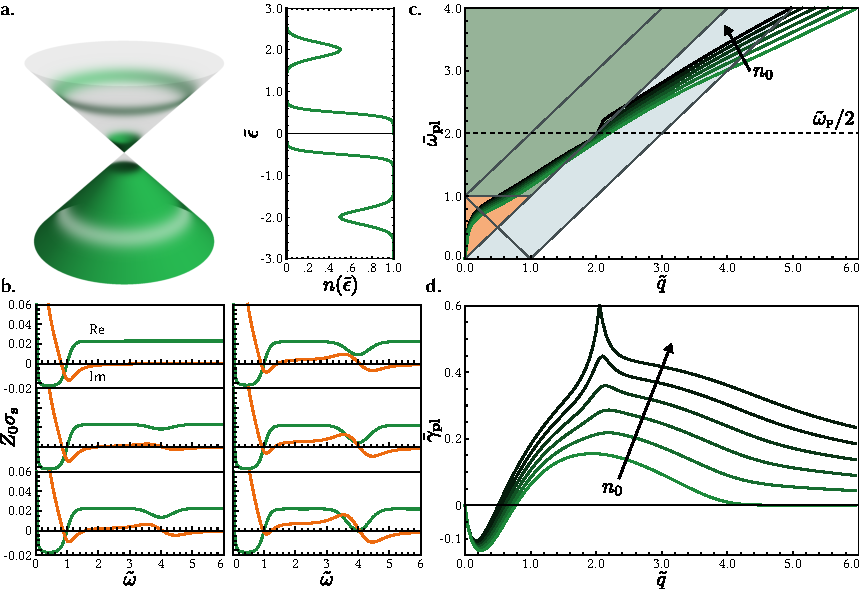
\includegraphics{figs/gr/HotDist.pdf}
 \caption[Polarisability of a hot electron distribution]{\label{fig:HotDist}
\textbf{Polarisability of a hot electron distribution.}\small\\
\subA. A hot carrier distribution of a symmetrically excited Gaussian
distribution of electrons and holes over a quasiequilibrium background
simulating photoinversion
\subB. The optical conductivity of this is plotted, for occupations levels
$n_0$, (the height of the Gaussian) between $0$ and $0.5$. 
Both real (green) and imaginary (orange) parts of the conductivity change about
the pump frequency, $\ωpump$.
\subC. Plasmon dispersions and \subD. losses for this polarisability are also
plotted.
The curves noticeably kink about the pump frequency $\ωpump$.
}
\end{figure}
The polarisability $\Π[n]$, calculated from \eq{simpleHot} with a Padé
approximant, is explored with parameter values of
$\ħ\ωpump/2 = 2\μbar$,
$\γpump = 0.175 \μbar$,
$\Ttil = 0.05$, and
$\μe = \μh$
in \fig{HotDist} for peak carrier occupations between $0$ and $0.5$.
Firstly, in a), the dimensionless conductivity is plotted for external optical
excitation, i.e. $q \→ 0$, $\ω \in \reals$, where,
\begin{equation}
  \Zf \σs(\qtilAbs, \ωtil)
= i \αf \frac{g}{2} \frac{\ωtil}{\qtilAbs^2}
  \Πtil(\qtilAbs, \ωtil)
\;.
\end{equation}
It can be seen that the real part of the conductivity, which at zero pump is
flat for $\ω \gtrsim 1$ begins to dip for increased pump strength at
$\ω = \ωpump$.
The corresponding imaginary part is modified for all frequencies centred about
this point as the refractive index changes.
The conductivity drops to zero at $\ω = \ωpump$ as the sheet is pumped to
transparency at $n_0 = 0.5$.

\FigSub{HotDist}{.b} and .c plots the plasmon dispersion and loss for this
polarisability configuration for varying occupation number.
The plasmon dispersion shifts everywhere, but most markedly at
$\ω = \ωpump/2$ where the steepness dramatically increases.
Perhaps surprisingly, there is no reduction in the plasmon loss at any frequency
despite carrier pairs being available for recombination.
This can be attributed to the change in refractive index morphing the plasmon
dispersion to exclude it from regions where there is phase-space for stimulated
recombination.
% Is this gain (anti-)guiding, is this similar to what has been seen in SLL?
This can be seen in the gain region ($\ωtil < 1$), where the gain is due to
quasiequilibrium photoinversion.
Here the gain decreases, not because there is any more phase-space for
absorption processes, but rather that the plasmon dispersion curve has steepened
in this region, leaving less phase space for the quasiequilibrium recombination
processes.
As the pump increases, this also induces a sharp peak of the loss around
$\vF q = \ωpump/2$, again this is about where the plasmon dispersion has been
perturbed the most.

This section has shown that the polarisability can be calculated as a functional
of arbitrary carrier distributions as a function of a complex variable.
The resulting plasmon dispersions from quasiequilibrium and a hot carrier
model have been shown.
A change in the carrier distribution can have a dramatic impact on the plasmon
dispersion and loss, though provisionally from what has been seen, wherever
there is a spread in carriers, there is an increase in the phase space opened up
for absorption processes that is not matched with an increase in emission
processes.

\section{Spontaneous Emission Spectrum} \label{sec:sponEmit}
There are three fundamental single particle excitation processes occurring in graphene:
spontaneous emission, stimulated emission, and stimulated absorption.
Spontaneous emission occurs when an electron in a higher energy state
transitions to occupy an empty state of lower energy, and a plasmon is emitted
in the process.
In absorption, an incoming plasmon is converted into an electron-hole pair, or
equivalently raises a lower energy electron into a higher unoccupied level.
Whereas in stimulated emission an incoming plasmon forces an electron to
transition into an unoccupied lower energy state, releasing an additional
plasmon in the process that is coherent with the first.
It is the processes of absorption and stimulated emission that induce Landau
gain or loss in plasmons, and therefore are responsible for the imaginary part
of the plasmon frequency $\γpl$, which is the net decay rate (absorption minus
emission),
\begin{equation}
2\γpl = \γplabs - \γplemit
\;,
\end{equation}
where the factor of 2 is because $\γpl$ is a \emph{field} decay rate,
whereas $\γplabs$ and $\γplemit$ are \emph{intensity} decay rates.

Spontaneous emission on the other hand does not enter into $\γpl$ but can be
calculated indirectly from it by considering the rate of plasmon decay for each
wavevector labelled plasmon state.
\begin{equation}
\pd{\npl(q)}{\t} = -\γplemit(q) (\npl(q) + 1)
\;.
\end{equation}
This is a sum of a stimulated part ($\npl(q)$) and a spontaneous part ($+1$)
The spectral rate of emission within a frequency interval $[\ω, \ω + \d\ω]$ is
extracted by taking the partial sum over all wavevector states,
\begin{subequations}\subeq
\begin{align}
\Rspon &= \frac{1}{A}\sum_\q \γplemit(q) = \int_{0}^\infty \d\ω \: \Gpl(\ω) \\
&= \int_{0}^\infty \d\ω \: \pd{q(\ω)}{\ω} \frac{q(\ω)}{2\π} \γplemit
\big( q(\ω) \big)
\;,
\end{align}
\end{subequations}
with the plasmon density of states,
$\Dpl = \pd{q(\ω)}{\ω} {q(\ω)} / {2\π}$,
and the \emph{inverse} of the plasmon dispersion relation $q(\ω)$, such that
$q \big( \ωpl(q) \big) = q$.
The plasmon spectral recombination rate areal density, $\Gpl$ is therefore given
as the plasmon emission rate $\γplemit$ weighted to the density of states
$\Dpl$ for plasmons in the frequency interval $[\ω, \ω + \d\ω]$.
From here the particle (or hole) recombination rate may be extracted, by
dividing through by the particle areal density to give the recombination rate of
electrons:
\begin{equation}
\Γple = \Rspon / N(\μe, \T)
\;,
\end{equation}
where $N(\μe, \T)$ is the particle number density in the conduction band.

It is not necessarily obvious how to extract the emission and absorption rates,
$\γplemit$ and $\γplabs$.
For zero temperature, these rates are mutually exclusive, i.e.
$\γplabs = 0 \text{ for } \γplemit \neq 0$ and vice-versa, since in the regions
where there is phase space for absorption processes, there is none for emission.
This is to say, the rates can be expressed with step functions,
\begin{subequations}\subeq \label{eq:zeroTRates}
\begin{align}
\γplemit(q) &= -2 \γpl(q) \θ( \μbar   - \ħ\ω(q) ) \\
\γplabs (q) &=  2 \γpl(q) \θ( \ħ\ω(q) - \μbar   )
\;.
\end{align}
\end{subequations}
For finite temperatures and hot carrier distributions, where the regimes overlap
each other, the situation is complicated.
Looking at the Lindhard formula \eq{lindhard}, there is a sum of distribution
functions, which is equivalent to the sum of a Fermi function product for the
phase space of each process.
\begin{equation}
n(\έ^s_{\k}) - n(\έ^{s'}_{\k+\q}) =
\underbrace{
n(\έ^s_{\k}) \Big( 1 - n(\έ^{s'}_{\k+\q}) \Big)
}_\text{Absorption} -
\underbrace{
n(\έ^{s'}_{\k+\q}) \Big( 1 - n(\έ^s_{\k}) \Big)
}_\text{Stimulated Emission}
\;,
\end{equation}
which is to say, the polarisability itself can be split up into,
\begin{equation}
\Π[n](\q, \ω) = \Σabs[n](\q, \ω) - \Σemit[n](\q, \ω)
\;,
\end{equation}
with,
\begin{equation}
\Σemit[n](\q,\ωpl) = \frac{g}{A} \Im \sum_{s,s'=\pm} \sum_{\k}
M^{s s'}_{\k,\k+\q}
\frac{
n(\έ^{s'}_{\k+\q}) \Big( 1 - n(\έ^s_{\k}) \Big)
}
{\έ^s_{\k} - \έ^{s'}_{\k+\q} + \ħ\ωpl + \i\times0}
\;,
\end{equation}
and an equivalent term for $\Σabs$.

The rates for the two individual processes can be calculated approximatively by
a \emph{Fermi's golden rule} (\fgr) expression.
Borrowing from the low-loss approximation \eq{lowloss}, the expression,
\begin{equation}
\γpl \approx V_q \Im \Π(\ωpl, q) \bigg/ \Re
\left.\pd{\εRPA}{\ω}\right|_{\ω=\ωpl}
\;.
\end{equation}
$\Π(\ωpl, q)$ can be split into absorption and emission components\footnote{
This step is not exact either, as the polarisability $\Π$ enters into $\εRPA$,
though as we will see, it makes a good approximation.
}
using $2\γpl = \γplabs - \γplemit$,
\begin{subequations}\subeq
\begin{align}
\γplabs \approx 2 V_q \Σabs(\ωpl, q) \bigg/ \Re
\left.\pd{\εRPA}{\ω}\right|_{\ω=\ωpl}
\\ \label{eq:γplemit}
\γplemit \approx 2 V_q \Σemit(\ωpl, q) \bigg/ \Re
\left.\pd{\εRPA}{\ω}\right|_{\ω=\ωpl}
\;.
\end{align}
\end{subequations}
This approximation may fair better than the low-loss approximation, since we can
put in the exactly solved real part of the dispersion.
This expansion will still start to break down as the Fermi line is approached,
though the emission term will fare much better than the absorption since, at
least for quasiequilibrium at moderate temperatures, the emission rate
approaches zero before the dispersion hits the Fermi line.
From here the absorption term can be derived from the exact net term as
$\γplabs = 2\γpl + \γplemit$.

The emission partial polarisability can be put into integrable form,
assuming only interband recombination processes are significant, as,
\begin{equation}
\Σemit(q,\ω)=
\frac{g q^2}{8 \π \ħ} \frac{\θ(\ω-\vF q)}{\sqrt{\ω^2-\vF^2 q^2}}
\int\limits_{-1}^{+1} \d u \: \sqrt{1-u^2}
n \left( \frac{\ħ\ω + \ħ \vF q u}{2} \right)
\bar{n} \left( \frac{\ħ \ω - \ħ \vF q u}{2} \right)
\;.
\end{equation}
which is derived in the appendix of \cite{Page2015}.

\begin{figure}
 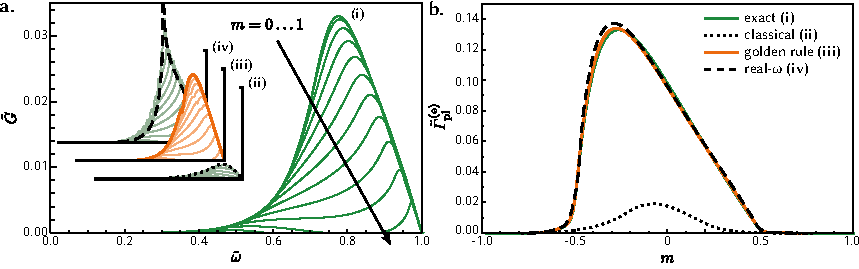
\includegraphics{figs/gr/SponZero.pdf}
 \caption[Spontaneous plasmon emission and electron recombination]{
 \label{fig:SponZero}
\textbf{Spontaneous plasmon emission and electron recombination.}\small\\
\subA. Plasmon spontaneous emission spectra, $\Gpltil$ and \subB. electron
recombination rates $\Γpletil$ at zero temperature.
Exact results derived from \cfpd curves (i) are plotted against approximate
results derived from \fgr for a classical Drude model (ii), \cfpd curves (iii),
and low-loss approximation.
Curves are dependent on carrier imbalance, $m$.
}
\end{figure}

The spontaneous emission is calculated and plotted in \fig{SponZero} for
zero temperature quasiequilibrium graphene, exactly (red lines) and in various
approximations.
Since for zero temperature, \eq{zeroTRates} holds and $\Gpl$ and $\Γple$ can be
calculated exactly [(i) in the figure] from the \cfpd using the directly
extracted $\γpl(q)$.
Three \fgr approximations are derived by calculating $\γplemit$ from
\eq{γplemit}, using the dispersion relations $\ωpl(q)$ from the classical Drude
model (ii), the \cfpd solution (iii), and the low-loss approximation;
curves which have been shown previously in \fig{PlasDisp}.
The exact result, obtained from the \cfpd will be used to test and
benchmark the appropriateness of \fgr solutions, which is important as
regimes where exact solutions cannot be obtained are explored.

The figure plots the dimensionless quantities
$\Gpltil = (\ħ\vF)^2\Gpl / \μbar^2$ and
$\Γpletil = \ħ\Γple / \μbar$,
which have the usual universality property\footnote{
$\Gpltil$ is scaled to the square of the energy scale $\μbar$ as it is an areal
density (\twod) quantity.
}.
Each set of curves in \figSub{SponZero}{.a} scans the spontaneous emission
spectrum over $\ωtil$ for varying levels of carrier inversion $m$.
The symmetrically inverted case $m=0$ acts as the envelope for each of the other
curves as the level of spontaneous emission drops with a reduction in inversion.
The curves all vanish to zero for $\ωtil > 1$ due to there being no phase space
outside this regime.
Of the approximative curves, the Drude model performs the worst, being a factor
of 5 slower than the exact solution.
This is due to a density of states that is an order of 10 times smaller than for
the other curves, despite having a raw emission rate $\γplemit$ that is larger
comparatively.
Using the low-loss approximation (iii) yields results that are the right order
of magnitude, but have spurious spikes in the curves which are a result of the
first order approximation overshooting when the dispersion curve passes near any
branch points.
The \cfpd dispersion approximation yields results that are most quantitatively
similar to the exact solution, though the match is not perfect and distinctive
dips are also observed near where the solution passes in the vicinity of branch
points.

In \figSub{SponZero}{.d}, each of the $\Gpltil$ curves are integrated over
frequency then scaled to the electron density to return the electron
recombination rate.
The equivalent procedure may be applied for holes and, due to particle-hole
symmetry, can be related as $\Γplhtil(m) = \Γpletil(-m)$.
The resulting curves are not themselves though symmetric about $m=0$ because for
electrons, for $m > 0$ they are the majority carrier, and for $m < 0$ the
minority and hence more sensitive to a change in carrier numbers.
The skew to the left indicates that the rate of electron recombination is
strongest when holes are the majority carrier, i.e. when for each electron, the
amount of holes available to recombine with is saturated.
The classical Drude limit has recombination rates a factor of 5 slower
than what is predicted using the exact formalism, and with
rates previously predicted in \cite{Rana2011}.
The other approximations work rather better in this picture, with any
inconsistencies that were present in the spectral form having been averaged out
in the recombination rate and largely matching the exact result.

In this formalism, carrier recombination rates are predicted to be a factor 5
faster than previously calculated.
When using representative energy scales, e.g. $\μbar = 0.2\eV$ yield
recombination times of $34\fs$ (at $m=0$).

Nonequilibrium Plasmon emission must therefore be considered as an important
channel for interband carrier recombination alongside the optical phonon
emission
\cite{Butscher2007,Rana2009,Wang2010,Yan2013}
and Auger recombination channels
\cite{Rana2007,Winzer2012,Tomadin2013,Brida2013}
when the dynamics of hot carriers in graphene are analysed
\cite{Breusing2011,Li2012,Gierz2013}.

\subsection{Recombination Rates at Finite Temperature and Collision Loss}
Armed with a reliable way to estimate spontaneous emission and \mdf
recombination rates, it remains to investigate how this changes with the
inclusion of finite temperature, or collision losses.

\begin{figure}
 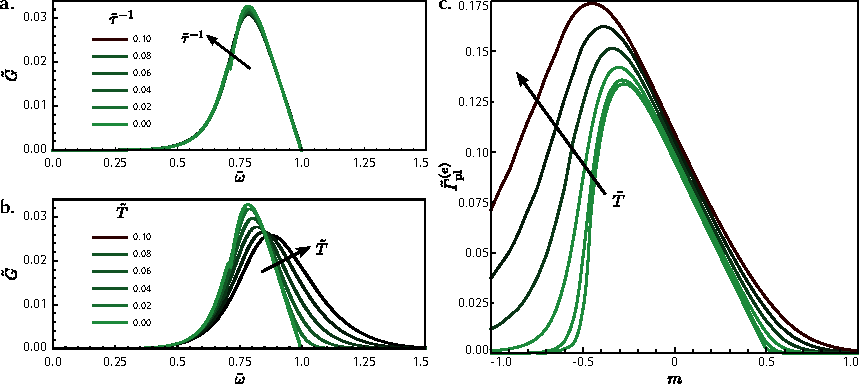
\includegraphics{figs/gr/SponTemp.pdf}
 \caption[Impact of temperature and collisions on spontaneous emission]
 {\label{fig:SponTemp}
 \textbf{Impact of temperature and collisions on spontaneous emission.}\small\\
Plasmon gain spectrum $\Gpltil(\ωtil)$ for intrinsic graphene ($m=0$) for:
\subA.
collision losses spanning $\τtil^{-1} \in [0,0.08]$, and \subB. temperatures
spanning $\Ttil^{-1} \in [0,0.1]$. Electron recombination rates over the same
temperature range are plotted in \subC over carrier imbalance $m$.
}
\end{figure}

By including collision loss and finite temperature effects, \eq{zeroTRates} no
longer holds, as the loss rate $\γpl$ is now not entirely due to recombination,
with added contributions from collision and Landau damping loss bleeding in.
In this situation the \fgr approximation of \eq{γplemit} must be used.
Curves for $m=0$ (representing the envelope) are plotted in the \cfpd \fgr
approximation for finite collision rates in \figSub{SponTemp}{.a} and finite
temperature in \figSub{SponTemp}{.b}.
In the case of collision loss, the rates hardly change at all.
This is because collision loss, although increasing the plasmon loss, is not a
recombination mechanism, and therefore does not contribute in the \fgr
expansion.
Any changes, including the smoothing out of the kink in the curve, are due to
the small changes in the dispersion curve from which the \fgr is calculated.

The situation for a finite temperature is quite different.
The character of the the emission rate $\γplemit$ shows a blueshift as the hard
edge at $\ωtil = 1$ for $\T = 0$ softens out to finite values for $\ωtil > 1$
as the phase space opens, much as was the case for the stimulated emission rates
(\fig{LowTemp}).
While the peak value of spontaneous emission decreases with temperature, the
spectrum as a whole broadens.
This can be seen most clearly in the \mdf recombination rates, which increase
with temperature for all values of $m$.
Again, when electrons are the minority carrier, their recombination rates are
more sensitive to changes in temperature, with increased phase space for
increased temperature.

The recombination time drops as temperature increases, from a value of $34\fs$
at zero temperature, as reported in the previous section, to a peak value of
$1/\Γple = 18\fs$ for $\T = 230\K$ and $m=-0.5$.

Summarising the results of this section, \fgr approximations of the emission and
absorption components of the plasmon rates have been shown.
The accuracy of these is critical on using the real part of the exactly solved
\cfpd solution, with approximative solutions (classical Drude model, and \rpa
polarisability in a low-loss approximation) giving results that are either
factors out, or with spurious features.
The emission rate can be used to calculate the spontaneous emission rates and
derived carrier recombination rates, which are found to be sensitive to
temperature, but insensitive to levels of collision losses.
The recombination rates are significantly faster than previously predicted and
must be considered in an analysis of carrier relaxation.

\section{Carrier Relaxation Dynamics} \label{sec:npe}
It was established in the previous section that spontaneous plasmon emission is
an ultrafast process in photoinverted graphene, with rates exceeding that of
optical phonon emission by orders of magnitude \cite{Rana2011}.
The resulting rates for carrier recombination indicate that plasmon emission may
be the dominant decay channel for nonequilibrium carrier relaxation in
graphene, a process that had been previously been attributed to Auger
recombination (\ar) \cite{Breusing2011,Brida2013}, which is subject to debate as
\ar processes are suppressed under \rpa dynamic screening models
\cite{Tomadin2013,Tielrooij2013}.

The recombination rates presented in the previous section are the instantaneous
values based on a fixed carrier distribution, whereas carrier recombination will
precisely seek to change the distribution over time.
In order to accurately predict how \emph{nonequilibrium plasmon emission}
(\npe) affects the carrier dynamics, a time-domain study of the carrier and
plasmon system becomes necessary together with additional recombination
pathways such as optical phonon emission, which may interplay and seek to take
heat out of the system.

For this section, the carrier system is assumed to relax instantaneously to
quasiequilibrium characterised by chemical potentials $\μe$ and $\μh$, for
electrons and holes respectively in the conduction and valence bands, and a
common carrier temperature $\Tc$, which feeds into Fermi carrier distributions
in each band as described in \sec{quasieq}.
Meanwhile the bosonic excitations, plasmons and optical phonons, are resolved by
wavevector $\nβ(\q)$ for each species bath, $\β$.

The carrier system's number and energy density moments, $\Ne$, $\Nh$, and $U$
evolve in time as driven by an external optical excitation pump term and due to
relaxation terms that couple to the boson baths.
\begin{subequations}\subeq
\begin{align}
\Ndote = \Ndoth &= \NdotPump - \NdotRel \\
\Udot &= \UdotPump - \UdotRel
\;.
\end{align}
\end{subequations}
Carriers are always generated pairwise as an electron and a hole, which results
in their rates being equal.

Assuming the system is pumped by a normally incident quasi-monochromatic,
$\ħ\ωpump$, planewave with a slowly varying envelope $I(\t)$, then the carrier
pairs excited and energy dissipated into the system is given by,
\begin{subequations}\subeq
\begin{align}
\NdotPump &= \Re [ \σsinter(\ω) ] |E(t)|^2 / (2\ħ\ω) \\
\UdotPump &= \Re [ \σs(\ω) ] |E(t)|^2 / 2 ,
\end{align}
\end{subequations}
where $\σs(\ω)$ is the optical conductivity ($q = 0$) as in \eq{condpol},
$\σsinter$ is the contribution to the sheet conductivity from interband
processes only, and $E(t)$ is the in plane component of the electric field
generated from a beam with an input intensity of $I(t)$, given as,
\begin{equation}
|E(t)|^2 =  2 \Zf \left|
\frac{1}{1 + \Zf \σs(\ω) / 2}
\right|^2
I(t)
\;,
\end{equation}
as derived from the \tmm formalism in \sec{stratmed}.

The system relaxes according to Boltzmann collision integrals, which account for
intraband scattering and interband recombination and pair generation processes.
Each boson field reservoir, $\β$, contributes to the number and energy density
relaxation rates.
Whereas only interband processes affect the number density, as these are the
processes that produce electron-hole pairs, both inter- and intraband processes
($\λ \in \{\ee,\hh,\eh\}$) relax the energy density,
\begin{subequations}\subeq
\begin{align}
\NdotRel &= \sum_\β \Rβ \\
\UdotRel &= \sum_{\β,\λ} \Sβλ
\;.
\end{align}
\end{subequations}
These rates themselves are summed over wavevector resolved processes, over each
band combination,
\begin{subequations}\subeq
\begin{align}
\Rβ &= \frac{1}{A} \sum_\q \rβeh(\q)\\
\Sβλ &= \frac{1}{A} \sum_\q \ħ\ω_\β(\q) \rβλ(\q)
\;.
\end{align}
\end{subequations}
with $\rβλ(\q)$ being the net spectral emission rate, including both
stimulated and spontaneous processes,
\begin{equation} \label{eq:netSER}
\rβλ(\q) = \γemit(\q) [\nβ(\q) + 1] - \γabs(\q) \nβ(\q)
\;.
\end{equation}
The bosonic fields themselves then relax via this interaction with the carrier
system, but additionally through decay processes through other channels
characterised by a relaxation rate $\nβdotrel(\q)$,
\begin{equation}
\nβdot = \sum_\λ \rβλ(\q) - \nβdotrel(\q)
\;.
\end{equation}
These additional relaxation processes can be phenomenologically modelled by a
characteristic time $\τβ$,
\begin{equation}
\nβdotrel(\q) = \τβ^{-1} \left[\nβ(\q) - \nβeq(\q,\Tamb)\right]
\;,
\end{equation}
where $\nβeq(\q,\Tamb)$ is the equilibrium distribution at an ambient
temperature $\Tamb$.

Initially a study of the carrier/plasmon system in isolation will be presented,
then optical phonons will be included.
The initial conditions for each simulation are the same; a pulse of fluence
$133 \μJ / \cm^2$ with frequency $\ħ\ω = 1\eV$ is incident on ambient
temperature intrinsic equilibrium graphene.
During excitation, in order that each initialisation is the same, relaxation
processes are turned off.
This leaves the system in an inverted state with $\μe = \μh \approx 0.3\eV$ and
$\Tc \approx 0.2\eV/\kB \: (2320\K)$.
As the system starts intrinsically doped $\μe = \μh$ and all carrier excitations
are pairwise, the electron and hole chemical potentials will remain equal, i.e.
a carrier imbalance of $m=0$, throughout the simulation.
The plasmon system is resolved isotropically in wavevector, i.e.
$\npl(\q) = \npl(q)$.

\begin{figure}
 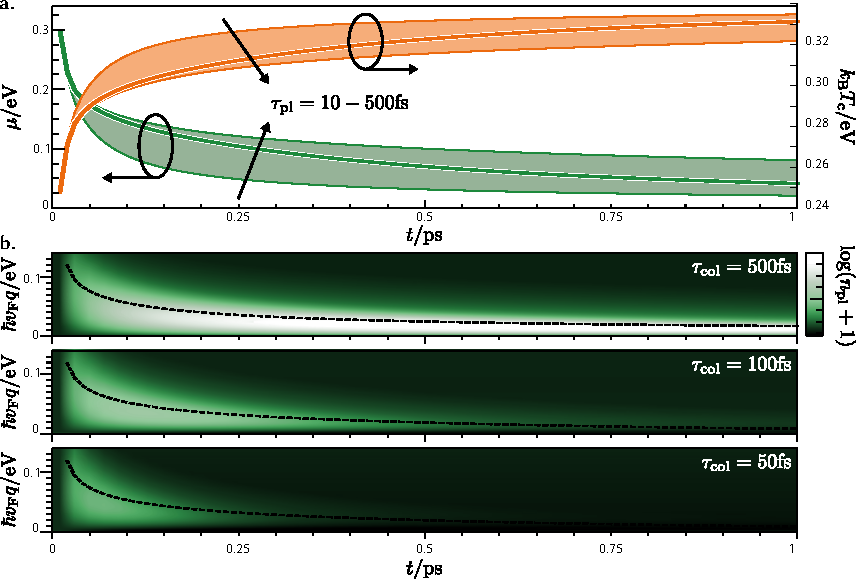
\includegraphics{figs/gr/NPERelax.pdf}
 \caption[Relaxation dynamics of coupled plasmon and carrier system]{
 \label{fig:NPERelax}
 \textbf{Relaxation dynamics of coupled plasmon and carrier system.}\small\\
\subA. Chemical potential (Green) and temperature (orange) of the carrier system
relaxing over time.
Solid lines are for a collision time $\τpl = 100\fs$ while shaded areas vary
from this in the range $\τpl \in [10,500]\fs$.
\\
\subB. shows the wavevector resolved plasmon occupation $\npl(q)$.
Black dashed lines mark the transition from absorption to emission.
}
\end{figure}

\subsection{Relaxation Via the Plasmon Channel}
The relaxation after excitation of the isolated carrier/plasmon system
(without optical phonons) is considered for a range of collision rates $\τpl$ in
the range $[10, 500]\fs$.
\Fig{NPERelax} shows how, in the first $1\ps$ after excitation, the carrier
system (a) and plasmon system (b) relaxes.
There is a sharp drop in inversion in the first $50\fs$ as the initially empty
plasmon bath is populated via interband recombination of carrier pairs.
The temperature correspondingly rises in this interval, which although the
energy density is dropping due to conversion to plasmons, the temperature must
rise such that the highest occupied carriers still have a probability of
occupation.
Plasmons may only be emitted at energies below $2\μ$, i.e. for $\γpl(\q) = 0$,
above this they are reabsorbed; the Fermi-edge drops over time meaning that
plasmons that were previously emitted may now be reabsorbed.
This reabsorption also increases the temperature, as there are many
electron-hole pair combinations that each plasmon may decay into, conserving
energy and momentum, despite having been created from a single particular
pair; this will seek to smear out the carrier distribution.
Over the next $200\fs$ the recombination rates slow down as inversion is
converted into temperature reducing the net emission of plasmons as in
\fig{TempScan}.
The dropping Fermi-edge means that plasmons that had been emitted
are being reabsorbed into the carrier system.
This slows down the decay rate of both the energy and number density which may
be described as a \emph{plasmon emission bottleneck}.
With an increasing collision loss, more plasmons are removed from the system, 
meaning that their energy is not being converted into electron-hole pairs,
lifting the bottleneck and allowing the carrier inversion to decay more
quickly.
This is most obviously noticed by comparing the steepness of the
outermost curves for the carrier temperature and chemical potential with
inversion lingering at $\μ = 0.1\eV$ for $\τpl = 500\fs$ but quickly depleting
at $\τpl = 10\fs$.

\subsection{Optical Phonons} \label{sec:optPhonons}
\begin{figure}
 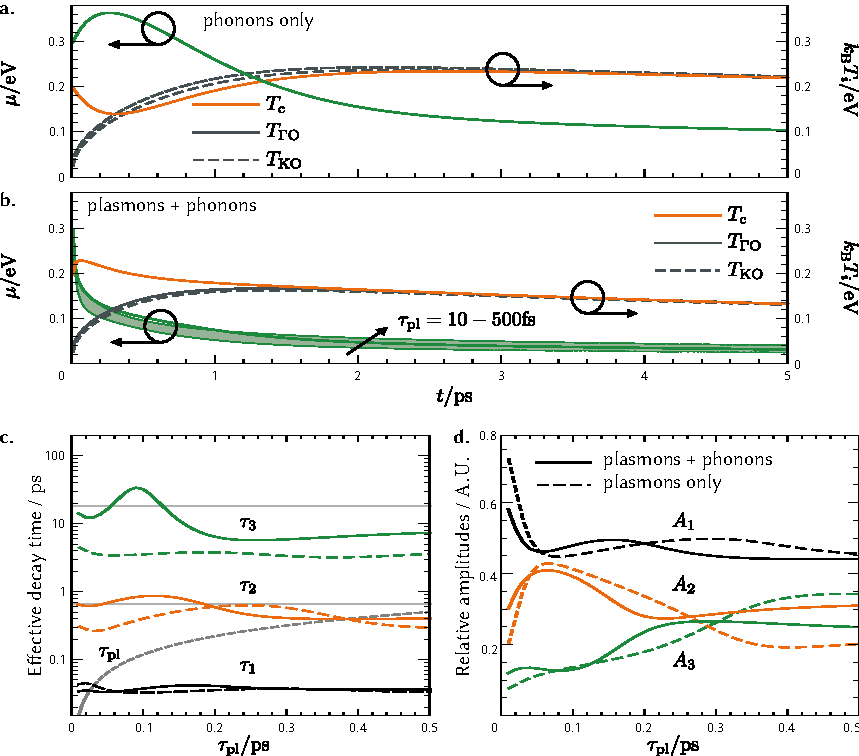
\includegraphics{figs/gr/NPERelaxPhon.pdf}
 \caption[Relaxation dynamics of carriers coupled plasmons and phonons]{
 \label{fig:NPERelaxPhon}
 \textbf{Relaxation dynamics of carriers coupled plasmons and phonons.}\small\\
\subA. Carrier temperature and chemical potential of carriers coupled only to
phonons, also shows the relaxation of phonon temperatures over time.
\subB. re-introduces plasmons, along with phonons, for varying collision times
$\τpl$.
\subC. and \subD. show extracted parameters ($A_i$, $\τ_i$) of a tri-exponential
fit of $\μ(t)$ for plasmons in isolation, and plasmons and phonons.
}
\end{figure}

Phonons also play a role in the relaxation of a hot carrier distribution
\cite{Wang2010},
being a channel for both intraband scattering \cite{Breusing2011} and interband
pair generation / recombination \cite{Rana2009}.
\emph{Longitudinal optical} (\LO) and \emph{transverse optical} (\TO) phonons
are the dominant channels for coupling to the carrier system.
They couple about the Γ and K symmetry points, allowing intra- and inter-valley
transitions respectively; about these points they are quasi-dispersion free
having a single frequency.
These are the \ΓO and \KO phonons, for which $\έΓO = 196\meV$,
$\έKO = 160\meV$.
There is also an acoustic phonon that couples at the K point
in this manner, \KA with $\έKA = 120\meV$.
Closed form expressions for the net spectral emission rates, as in \eq{netSER},
can be derived due to the dispersion free nature of the modes, and are presented
in the supplementary material of Ref~\cite{Hamm2015}.

\FigSub{NPERelaxPhon}{.a} shows how the carrier system relaxes in the
presence of only the phonons, i.e. with plasmons not included.
The phonons are modelled to follow a Bose-Einstein distribution with a separate
temperature for each phonon species.
Since each species is mono-energetic, the temperature will uniquely determine
the occupation number of that species.
Such description assumes an instantaneous relaxation of the phonons to be
uniformly distributed over wavevector.
The phonon relaxation time is assumed to be $\τph = 2.5\ps$ \cite{Wang2010}.

In the first $500\fs$ the carrier temperature drops accompanied by an increase
in chemical potential and a rise in phonon temperatures.
This is indicative of intraband scattering, where the number density stays the
same, but energy is transferred from the carriers to phonons.
Once the phonon and carrier temperatures match, they then largely follow each
other, slowly decreasing as phonons are emitted from interband recombination of
carriers.

Next plasmons and phonons are simulated together, the trace of carrier and
phonon configuration is given in \figSub{NPERelaxPhon}{.b}.
Initially inversion drops sharply as plasmons are emitted, but this is not
accompanied by a sharp rise in carrier temperature, as was the case with
plasmons alone, as the coupling with phonons removes excess temperature from the
carrier plasma through intraband emission.
Again, once the carrier and phonon temperatures have equalised after around
$1\ps$, the inversion slowly drains, albeit, in contrast to with phonons alone,
the chemical potential has by now been significantly cut.
With an increase in the plasmon decay rate, energy is removed from the system
faster, though with the phonons now acting as an efficient channel to extract
heat, this effect is less sensitive to the decay rate than with plasmons alone.

Further inferences can be made by examining the characteristic of the chemical
potential drop in more detail.
A tri-exponential function,
$\μ = \μ_0 \sum_{i=1}^3 A_i \exp(-t / \τ_i)$,
can be fit to the time evolution.
\FigSub{NPERelaxPhon}{.c} shows this fit for both \npe alone and \npe with
phonons, as plasmon collision loss varies.
The timescales that emerge ($\τ_1$, $\τ_2$, $\τ_3$) separate out into distinct
values that are largely independent on the collision loss.
The fastest timescale, $\τ_1 \approx 0.03\ps$ represents the filling of the
initially empty plasmon bath via spontaneous recombination of electron-hole
pairs.
The amplitude, $A_1$, of this timescale is steady for $\τpl > \τ_1$, though in
the opposite limit, where plasmons are absorbed at a faster rate than they are
created, the amplitude shoots up as most of the energy is extracted from the
system in this way.
The second timescale $\τ_2 \approx 0.3\ps$ is associated with the conversion of
inversion to temperature, by emitting plasmons below the Fermi-edge, the edge
dropping, and the same plasmons re-absorbing above it.
The amplitude $A_2$, of this process drops as $A_1$ rises when plasmons are
quickly dissipated for $\τpl < \τ_1$, this is because there will be no plasmons
in the bath to re-absorb back into the carrier system.
The final rate $\τ_3$ represents the remaining drain of energy as the saturated
plasma bath depletes.
As the collision loss increases, $\τpl \gtrsim 0.2\ps $, the proportion of the
inversion lost through this mechanism increases, thereby depleting the next
slowest rate amplitude $A_2$.
This channel is the only one whose rate is significantly affected by the
inclusion of phonons, with the characteristic time $\τ_3$ universally
increasing; this can be attributed to the phonons being a separate store of
energy that is passed through before exiting the system.

Overall, the dependence on collision loss only affects the dynamics
significantly if it is small enough to empty the plasmon bath faster than it is
filled, at $\τpl \lesssim 0.2\ps$.
The addition of phonons into the model however most strongly influences the
dynamics by slowing down the decay of inversion and reducing its dependence on
the plasmon relaxation rate.

This establishes that \npe acts as an efficient mechanism for the equilibration
of thermal photoinverted graphene.
Hot electron-hole pairs may recombine creating a plasmon, removing energy and
carriers from the \mdf plasma.
This energy is re-distributed back to the carrier system and through phonon
channels to eventually be removed from the system as the plasmon bath is
depleted due to electron collisions.
The predictions are self-consistent and in agreement with experimental findings
\cite{Li2012} without requiring arbitrary tuning.

\section{Conclusions}
This chapter has introduced a method of calculating the polarisability of
graphene for arbitrary carrier distributions in the Dirac cone approximation.
This has allowed for the calculation of the complex frequency plasmon dispersion
curves, which are exact solutions of the poles of the Coulomb potential in \rpa.
The complex nature of the solution encodes in its imaginary part the rates of
loss and gain for plasmons in regions where there is coupling through
absorption and stimulated emission to the \mdf plasma.
By calculating the emission spectrum, this work gives
indication that plasmons with gain can indeed exist in graphene under realistic
conditions.

The resilience of the plasmons under conditions of collision loss, finite
temperature, and chemical doping has been demonstrated.
The modal loss added by the inclusion of collisions is proportional to the
inverse of the collisional lifetime, whereas the effects of temperature and
doping is to blueshift the frequency of the peak loss rate.
The dispersion of the plasmons is largely unaffected by collisions and low
temperatures, but sensitive to doping, exhibiting a critical splitting in the
families of curves observed.
The plasmons of hot nonequilibrium carriers are shown to have strong dependency
on the carrier distribution.

Spontaneous emission, that accompanies the stimulated gain, is also described in
this model.
A Fermi's golden rule scheme allows for the extraction of the spontaneous
plasmon emission spectrum, but also for the carrier recombination rates.
These are calculated under the effects of collision, temperature, and
doping.
While collisions do not contribute to this channel, temperature and doping have
a strong influence.
The rates calculated for nonequilibrium graphene are shown to be a factor 5
times faster than previously estimated.
This suggests that plasmons play a key role in the dynamics of hot carrier
inversion decay, that has been observed in pump-probe and \trarpes experiments.

The dynamics of carrier relaxation is investigated in interaction with plasmon
and phonon reservoirs.
It is shown that by emitting into the plasmon channels, energy can be removed
from the carrier system on $100\fs$ timescales, which is consistent with recent
experimental results \cite{Breusing2011,Li2012}.
 % Chapter 4 - Graphene
\clearpage~\clearpage
\chapter{Conclusion}

This thesis has been themed on controlling light in two dimensions with active
plasmonics.
Two particular topics were focused on, stopped light lasing and gain in
nonequilibrium graphene, where in both plasmons are coupled to electronic
systems to exploit the stimulated emission into plasmonic channels.

The question asked of stopped light was:
By controlling the dispersion relation of light in a plasmonic waveguide such
that energy is brought to rest at zero group velocity within a gain medium, can
a regime of lasing be entered without a cavity storing the light in a resonant
mode?

Designing a structure than not only stops light, but minimises the dispersion
over a large range of wavevectors, allows a wavepacket to be formed that
localises over a gain medium.
The localisation derives from balanced and opposing energy flows in metallic and
dielectric layers that form vortices around the edges of the gain medium.
Lasing is indeed shown to be possible;
time domain simulations show the transition from amplified spontaneous emission
to lasing via characteristic relaxation oscillations.

The dynamics of the lasing mode are unusual.
Energy is localised, but the mode does not form a in standing wave, but rather a
propagating one with zero group velocity.
This is analogous to a barber’s pole, where the stripes are continually moving
but the pole stays in place.
The stopped light laser is a source of coherent plasmons that are well
described with a complex wavevector.
This is in contrast to the lasing mode itself which is described with complex
frequencies.

From here, there are a number of avenues one may take to build on this work.
Firstly, simulations have been done in \twod
(one dimension parallel to the structure, $x$, and the other perpendicular, $z$
).
In the third (homogenised) dimension, $y$, emitters are coherent with
each other and of equal inversion.
In \threed this need not be the case.
Additionally, polarisation effects that were not present in \twod become
available adding extra dynamics that must be studied.

This all should lead to an experimental realisation of a stopped light
structure.
Theoretical models and simulations should be geared to inform the design of a
structure that can be fabricated in the lab, accounting for imperfections and
variations not present in the idealised model.

Turning to graphene, the question posed in the introduction can now be answered:
If graphene is optically pumped such that its carriers enter a state of
inversion, are plasmon modes supported and can the inversion compensate for any
material losses and lead to amplification of the plasmons?

Graphene has been shown to support plasmons with gain, including under realistic
conditions of finite temperature, chemical doping, and collision loss.
In order to arrive at this answer a model for calculating polarisabilities for
nonequilibrium carrier distributions was derived and this allowed for the
calculation of complex-frequency plasmon dispersion relations which encode the
gain and loss.

It has also been shown that the relaxation of hot carrier distributions is
ultra-fast due to spontaneous broadband nonequilibrium emission of plasmons on
a timescale of $\sim100\fs$.
This is in agreement with experimental findings that have thus far relied on
theoretically suppressed Auger processes to justify the observed rates.

To build on this work, one may wish to consider multi-layer graphene or other
\twod materials such as \tmds.
The model for calculating nonequilibrium polarisabilities is not specific to
monolayer graphene, and could be applied to such materials, and indeed to
models of monolayer graphene beyond the Dirac cone approximation.
This could lead to the construction of graphene based plasmonic devices, beyond
suspended graphene, or graphene on a simple substrate that has been considered
here.

Another extension worth considering is anisotropic excitation:
When graphene is photoexcited, carriers pairs are produced with a definite
momentum distribution on the cone.
At present, this can not be modelled in this framework, but should be
investigated in order to consider the dynamics of photoexcitation more fully.

An obvious question that arises from this thesis is can the topics of graphene
and stopped light be combined to form a graphene plasmonic stopped light laser?
The fast inversion relaxation and a broadband spontaneous emission of graphene
make it unsuitable for lasing by itself.
However, this could be mitigated by using graphene as the metallic component of
an \sl structure, not as the emitter, and a \tmd for the semiconductor.
\textsc{Tmd}s have a finite direct bandgap which should make them ideal for such
a purpose.
This would allow for a stopped light laser where, not only is the mode
subwavelength, but the entire device is too.
 % Chapter 5 - Conclusion
\clearpage~\clearpage

\renewcommand*{\chapterformat}{}
\appendix
\chapter{Appendices}

\renewcommand*{\chaptermarkformat}{}
\section{Plots of Functions of a Complex Variable} \label{sec:f(z)}
\chaptermark{Appendix 1. Plots of Functions of a Complex Variable}

\begin{figure}
 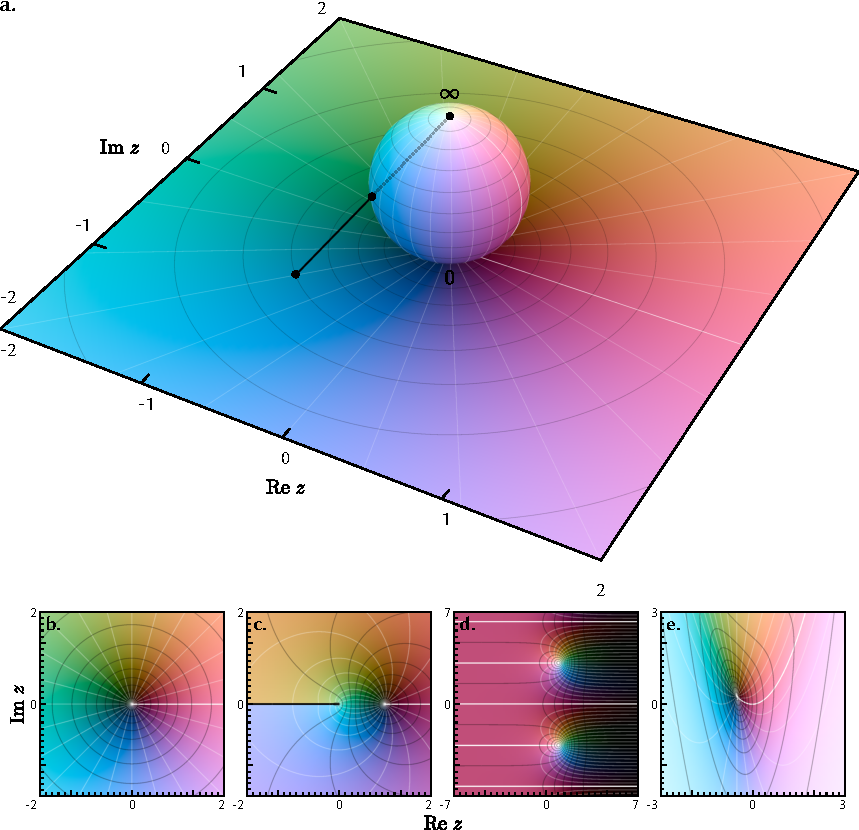
\includegraphics{figs/app/Riemann.pdf}
 \caption[Riemann sphere and complex plots]{\small \label{fig:riemann}
 \textbf{Riemann sphere and complex plots.}\small\\
 \subA. projection of the Riemann sphere onto the complex plane, each point on
 the sphere is assigned a unique colour, which maps to the extended complex
 plane.\\
 \subB, \subC, \subD, \subE. show complex plots of the following functions:
 \\
 \subB. Identity function, $f(z) = z$, zeros show in black as sources of contour
 lines.
 \\
 \subC. Logarithm, $f(z) = \log z$, note the branch cut along the negative real
 axis.
 \\
 \subD. Fermi Function, $f(z) = (1+\exp(z-1))^{-1}$, poles here are shown in
 white and are sinks of contour lines.
 \\
 \subE. Non-analytic function, $f(x+iy)=1+2 x + i y - i x^2$. Non-analytic
 functions are not conformal maps in the complex plane, producing contours that
 do not intersect at right angles.
 }
\end{figure}

In this thesis, it has occasionally been necessary to plot functions of a complex
variable.
These functions are often difficult to visualise since they map one pair of
real variables to another $f: x + i y \→ u + i v$, requiring four dimensions
in total for the domain and the range.

Here functions of a complex variable are plotted as \twod colour plots, where
the range of the function is mapped to a colour that is plotted over the domain.

Colours are assigned such that every point on the extended complex plane
$\hat{\mathbb{C}}$ (Complex numbers and the point at infinity) is uniquely
coloured.
Here $\hat{\mathbb{C}}$ is mapped to the Riemann sphere,
defined as the points labelled with polar angles $(\θ,\φ)$ on a sphere of radius
$\nicefrac{1}{2}$ that touches the complex plane at $0$ at its base, as depicted
in \fig{riemann}.
Points on the complex plane are mapped to the sphere by a construction where a
line is drawn from the top of the sphere to a point on the plane; the point is
mapped to the intersection of that line and the sphere.
This is expressed more concisely as $(\θ(r), \φ) = r e^{i\φ} \→ (2
\arccot r,\φ)$.

The sphere is coloured in a CIE L*a*b* colour space, with the top point being
white, the bottom black, with the saturation maximal around the equator
(representing unit complex numbers).
The phase maps to the hue of the colour, with red being real positive
numbers.
The \emph{lab} colour space has the advantage that it is “perceptually uniform”,
which is to say that colours that vary only by hue, look the same brightness and
saturation to a human eye.
This will avoid spurious bright bands that appear in an sRGB colour space.

In the plots, contours are drawn for constant amplitude in black, and constant
phase in white.
Analytic functions are conformal maps - they preserve angles, therefore plots of
analytic functions will have their contours intersect at right-angles (except at
singular points and zeros, and points of zero derivative).
In such a depiction, roots and poles are sources and sinks of contours of
constant phase, and are circled by contours of constant amplitude, with roots
being a black point, and poles being a white point.
Branch points are drawn in this plot as thicker black lines.
This is depicted in examples in \fig{riemann} in addition to a function that is
not analytic hence not a conformal map.

\section{Branches of the Polarisability Function} \label{sec:branchcuts}
\chaptermark{Appendix 2. Branches of the Polarisability Function}

The dimensionless polarisability of zero temperature doped graphene, given in
\eq{analPolar}, is a multi-valued function of a complex variable.
The function, as given, has branch cuts, and a straight evaluation will return
the principal branch.
In the analysis of \sec{cfpd}, it can be required that the function needs to be
analytically continued over a branch cut.

Here the functions $\Πtil_1$, $\Πtil'$, and $\Πtil_0$ are presented as functions
of a complex $\ωtil$ for constant $\qtil$, with the additional dependence of a
branch parameter $\ξ$, which is a list of integers.

The original functions are,
\begin{subequations}\subeq
\begin{align}
\Πtil_1(\qtil, \ωtil) &=
-4 + \qtilAbs^2 \frac{G^{+}(\frac{2+\ωtil}{\qtilAbs}) +
G^{-}(\frac{2-\ωtil}{\qtilAbs})}{2
\sqrt{\qtilAbs^2 - \ωtil^2}}
\\
\Πtil'(\έtil; \qtil, \ωtil) &=
-4 + 2 \frac{
\Gp \left( \frac{\ωtil + 2 \έtil}{\qtilAbs} \right) +
\Gp \left( \frac{\ωtil - 2 \έtil}{\qtilAbs} \right)
}{
\Gp \left( \frac{\ωtil}{\qtilAbs} \right)
}
\\
\Πtil_0(\qtil, \ωtil) &= -\frac{\qtilAbs}{2} \frac{\π}{\Gp \left(
\frac{\ωtil}{\qtilAbs} \right) }
\;,
\end{align}
\end{subequations}
with,
\begin{subequations}\subeq
\begin{align}
G^{\pm}(z) &= z \sqrt{1-z^2} \pm \i \arccosh(z)
\\
\Gp(z) &= \sqrt{1 - z^2}
\;.
\end{align}
\end{subequations}
The branch cuts originate from square-root and logarithmic (arccosh) branch
point singularities.

Redefining the auxiliary functions as,
\begin{subequations}\subeq
\begin{align}
\Gp_{m,n}(z) &=
e^{i \π/2 (n + m)} \sqrt{e^{-i \π (n + 1/2)} (z - 1)} \sqrt{
  e^{-i \π (m + 1/2)} (z + 1)}
\\
G_{m,n,p}(z) &=
z \Gp_{m, n}(z) + i \log\left(e^{-i \π (p + 1/2)} (z + i \Gp_{m, n}(z))\right)
- \π p
\;.
\end{align}
\end{subequations}
sets each branch cut to be angled vertically downwards along the negative
imaginary axis.
$m$ controls the branch cut at $z=-1$ and $n$ at $z=+1$.
By incrementing or decrementing this value, the branch is rotated
counter-clockwise 180°.
$p$ controls the branch of the logarithm, is set such that it's branch cut is
not exposed, but is rather hidden in the other leaf of the square root.

The polarisability functions can then be set such that all the branch cuts point
downwards in $\ωtil$.
In the general case, this is controlled by eight integers:
\begin{subequations}\subeq
\begin{align}
\Πtil_1(\qtil, \ωtil; \ξ) &=
-4 + \qtilAbs \frac{
G_{\ξ_1, \ξ_2, \ξ_3}\left( \frac{\ωtil + 2}{\qtilAbs} \right) -
G_{\ξ_6, \ξ_7, \ξ_8}\left( \frac{\ωtil - 2}{\qtilAbs} \right) - \π
}{
2 \Gp_{\ξ_4, \ξ_5}\left( \frac{\ωtil}{\qtilAbs} \right)
}
\\
\Πtil'(\έtil; \qtil, \ωtil; \ξ) &=
-4 + 2 \frac{
\Gp_{\ξ_1, \ξ_2}\left(\frac{\ωtil + 2\έtil}{\qtilAbs}\right) +
\Gp_{\ξ_6, \ξ_7}\left(\frac{\ωtil - 2\έtil}{\qtilAbs}\right)
}{
\Gp_{\ξ_4, \ξ_5}\left(\frac{\ωtil}{\qtilAbs}\right)
}
\\
\Πtil_0(\qtil, \ωtil; \ξ) &= -\frac{
\π \qtilAbs
}{
2 \Gp_{\ξ_4,\ξ_5}\left( \frac{\ωtil}{\qtilAbs} \right)
}
\;.
\end{align}
\end{subequations}
As with the auxiliary $G$ functions, incrementing $\ξ_i$ will rotate its
associated branch by 180° counter-clockwise.
When tracing roots, each time the root moves from the upper half-space to the
lower or vice-versa, each branch cut should be determined to rotate either
clockwise or counter-clockwise such that it does not cross over the root.
 % Appendices

\clearpage~\clearpage

\renewcommand{\v}[1]{\hacek{#1}}
\small
\bibliography{references}

\end{document}